\documentclass[twoside]{book}

% Packages required by doxygen
\usepackage{fixltx2e}
\usepackage{calc}
\usepackage{doxygen}
\usepackage[export]{adjustbox} % also loads graphicx
\usepackage{graphicx}
\usepackage[utf8]{inputenc}
\usepackage{makeidx}
\usepackage{multicol}
\usepackage{multirow}
\PassOptionsToPackage{warn}{textcomp}
\usepackage{textcomp}
\usepackage[nointegrals]{wasysym}
\usepackage[table]{xcolor}

% Font selection
\usepackage[T1]{fontenc}
\usepackage[scaled=.90]{helvet}
\usepackage{courier}
\usepackage{amssymb}
\usepackage{sectsty}
\renewcommand{\familydefault}{\sfdefault}
\allsectionsfont{%
  \fontseries{bc}\selectfont%
  \color{darkgray}%
}
\renewcommand{\DoxyLabelFont}{%
  \fontseries{bc}\selectfont%
  \color{darkgray}%
}
\newcommand{\+}{\discretionary{\mbox{\scriptsize$\hookleftarrow$}}{}{}}

% Page & text layout
\usepackage{geometry}
\geometry{%
  a4paper,%
  top=2.5cm,%
  bottom=2.5cm,%
  left=2.5cm,%
  right=2.5cm%
}
\tolerance=750
\hfuzz=15pt
\hbadness=750
\setlength{\emergencystretch}{15pt}
\setlength{\parindent}{0cm}
\setlength{\parskip}{3ex plus 2ex minus 2ex}
\makeatletter
\renewcommand{\paragraph}{%
  \@startsection{paragraph}{4}{0ex}{-1.0ex}{1.0ex}{%
    \normalfont\normalsize\bfseries\SS@parafont%
  }%
}
\renewcommand{\subparagraph}{%
  \@startsection{subparagraph}{5}{0ex}{-1.0ex}{1.0ex}{%
    \normalfont\normalsize\bfseries\SS@subparafont%
  }%
}
\makeatother

% Headers & footers
\usepackage{fancyhdr}
\pagestyle{fancyplain}
\fancyhead[LE]{\fancyplain{}{\bfseries\thepage}}
\fancyhead[CE]{\fancyplain{}{}}
\fancyhead[RE]{\fancyplain{}{\bfseries\leftmark}}
\fancyhead[LO]{\fancyplain{}{\bfseries\rightmark}}
\fancyhead[CO]{\fancyplain{}{}}
\fancyhead[RO]{\fancyplain{}{\bfseries\thepage}}
\fancyfoot[LE]{\fancyplain{}{}}
\fancyfoot[CE]{\fancyplain{}{}}
\fancyfoot[RE]{\fancyplain{}{\bfseries\scriptsize Generated by Doxygen }}
\fancyfoot[LO]{\fancyplain{}{\bfseries\scriptsize Generated by Doxygen }}
\fancyfoot[CO]{\fancyplain{}{}}
\fancyfoot[RO]{\fancyplain{}{}}
\renewcommand{\footrulewidth}{0.4pt}
\renewcommand{\chaptermark}[1]{%
  \markboth{#1}{}%
}
\renewcommand{\sectionmark}[1]{%
  \markright{\thesection\ #1}%
}

% Indices & bibliography
\usepackage{natbib}
\usepackage[titles]{tocloft}
\setcounter{tocdepth}{3}
\setcounter{secnumdepth}{5}
\makeindex

% Hyperlinks (required, but should be loaded last)
\usepackage{ifpdf}
\ifpdf
  \usepackage[pdftex,pagebackref=true]{hyperref}
\else
  \usepackage[ps2pdf,pagebackref=true]{hyperref}
\fi
\hypersetup{%
  colorlinks=true,%
  linkcolor=blue,%
  citecolor=blue,%
  unicode%
}

% Custom commands
\newcommand{\clearemptydoublepage}{%
  \newpage{\pagestyle{empty}\cleardoublepage}%
}

\usepackage{caption}
\captionsetup{labelsep=space,justification=centering,font={bf},singlelinecheck=off,skip=4pt,position=top}

%===== C O N T E N T S =====

\begin{document}

% Titlepage & ToC
\hypersetup{pageanchor=false,
             bookmarksnumbered=true,
             pdfencoding=unicode
            }
\pagenumbering{alph}
\begin{titlepage}
\vspace*{7cm}
\begin{center}%
{\Large A\+G\+AL }\\
\vspace*{1cm}
{\large Generated by Doxygen 1.8.13}\\
\end{center}
\end{titlepage}
\clearemptydoublepage
\pagenumbering{roman}
\tableofcontents
\clearemptydoublepage
\pagenumbering{arabic}
\hypersetup{pageanchor=true}

%--- Begin generated contents ---
\chapter{Hierarchical Index}
\section{Class Hierarchy}
This inheritance list is sorted roughly, but not completely, alphabetically\+:\begin{DoxyCompactList}
\item \contentsline{section}{Mesh}{\pageref{classMesh}}{}
\item \contentsline{section}{Solver}{\pageref{classSolver}}{}
\begin{DoxyCompactList}
\item \contentsline{section}{Solver\+\_\+\+L\+BM}{\pageref{classSolver__LBM}}{}
\end{DoxyCompactList}
\end{DoxyCompactList}

\chapter{Class Index}
\section{Class List}
Here are the classes, structs, unions and interfaces with brief descriptions\+:\begin{DoxyCompactList}
\item\contentsline{section}{\hyperlink{classMesh}{Mesh} \\*The mesh class }{\pageref{classMesh}}{}
\item\contentsline{section}{\hyperlink{classSolver}{Solver} }{\pageref{classSolver}}{}
\item\contentsline{section}{\hyperlink{classSolver__LBM}{Solver\+\_\+\+L\+BM} }{\pageref{classSolver__LBM}}{}
\end{DoxyCompactList}

\chapter{File Index}
\section{File List}
Here is a list of all files with brief descriptions\+:\begin{DoxyCompactList}
\item\contentsline{section}{inc/\hyperlink{cppspec_8h}{cppspec.\+h} }{\pageref{cppspec_8h}}{}
\item\contentsline{section}{inc/\hyperlink{lbm_8h}{lbm.\+h} }{\pageref{lbm_8h}}{}
\item\contentsline{section}{inc/\hyperlink{main_8h}{main.\+h} }{\pageref{main_8h}}{}
\item\contentsline{section}{inc/\hyperlink{mesh_8h}{mesh.\+h} }{\pageref{mesh_8h}}{}
\item\contentsline{section}{inc/\hyperlink{solver_8h}{solver.\+h} }{\pageref{solver_8h}}{}
\end{DoxyCompactList}

\chapter{Class Documentation}
\hypertarget{classMesh}{}\section{Mesh Class Reference}
\label{classMesh}\index{Mesh@{Mesh}}


The mesh class.  




{\ttfamily \#include $<$mesh.\+h$>$}

\subsection*{Public Member Functions}
\begin{DoxyCompactItemize}
\item 
int \hyperlink{classMesh_a054ca03cc4a2c7d2fd01db790855a066}{M\+\_\+\+Print} (int i\+\_\+dev, int iter)
\begin{DoxyCompactList}\small\item\em Print the mesh. \end{DoxyCompactList}\item 
int \hyperlink{classMesh_a4d6deb8379e8f8573d17915a14eede30}{M\+\_\+\+Print\+Connectivity} (int i\+\_\+dev)
\begin{DoxyCompactList}\small\item\em \mbox{[}D\+E\+B\+UG\mbox{]} Print connectivity output. \end{DoxyCompactList}\item 
int \hyperlink{classMesh_a18eb5172a0fc6167fe37c357ad3ef345}{M\+\_\+\+Load\+To\+G\+PU} ()
\begin{DoxyCompactList}\small\item\em Transfer data structures from C\+PU to G\+PU. \end{DoxyCompactList}\item 
int \hyperlink{classMesh_a19de000974249ca4f03b00e1cf2a8f5d}{M\+\_\+\+Retrieve\+From\+G\+PU} ()
\begin{DoxyCompactList}\small\item\em Transfer data structures from G\+PU to C\+PU. \end{DoxyCompactList}\item 
int \hyperlink{classMesh_a6350653aaf7e0115ebc8e47f97bde421}{M\+\_\+\+Freeze\+Refined\+Cells} (int var)
\begin{DoxyCompactList}\small\item\em Freeze (or unfreeze) the current status of refinement in the grid. \end{DoxyCompactList}\item 
int \hyperlink{classMesh_a7f1c861db5b8168cff9dabf728c0ce1a}{M\+\_\+\+Refine\+And\+Coarsen\+Cells} (int var, \hyperlink{cppspec_8h_af529d360dfac9b9578aa719418a53a21}{ufloat\+\_\+t} $\ast$scale\+\_\+vec, std\+::ofstream $\ast$file)
\begin{DoxyCompactList}\small\item\em Perform refinement and coarsening wherever marked. \end{DoxyCompactList}\item 
int \hyperlink{classMesh_aeb91bf44cbf5e9edfa52e8ac06d003ce}{M\+\_\+\+Interpolate} (int i\+\_\+dev, int L, int var, \hyperlink{cppspec_8h_af529d360dfac9b9578aa719418a53a21}{ufloat\+\_\+t} Cscale=0)
\begin{DoxyCompactList}\small\item\em Interpolate values between grid levels. \end{DoxyCompactList}\item 
int \hyperlink{classMesh_a4c0709e00c84ca8957713f681cad1897}{M\+\_\+\+Average} (int i\+\_\+dev, int L, int var, \hyperlink{cppspec_8h_af529d360dfac9b9578aa719418a53a21}{ufloat\+\_\+t} Cscale=0)
\begin{DoxyCompactList}\small\item\em Average between grid levels. \end{DoxyCompactList}\item 
int \hyperlink{classMesh_ad70a286b2d0da0c8b1f7de939bb5d65e}{M\+\_\+\+Cuda\+Mod\+Vals} (int var)
\begin{DoxyCompactList}\small\item\em \mbox{[}D\+E\+B\+UG\mbox{]} Modify specific values in data arrays on the G\+PU. \end{DoxyCompactList}\item 
int \hyperlink{classMesh_aa8af131d960c3a98cba329620a678ab4}{M\+\_\+\+Print\+Last\+N\+Gaps} (int i\+\_\+dev, int N)
\begin{DoxyCompactList}\small\item\em \mbox{[}D\+E\+B\+UG\mbox{]} Print the last N gaps from the gap set. \end{DoxyCompactList}\item 
\hyperlink{classMesh_a2af137f1571af89172b9c102302c416b}{Mesh} ()
\begin{DoxyCompactList}\small\item\em Default constructor. \end{DoxyCompactList}\item 
\hyperlink{classMesh_ae13aff57d73893651b5386ecdba97cd3}{Mesh} (int $\ast$Nxi\+\_\+, double dx\+\_\+)
\begin{DoxyCompactList}\small\item\em Main constructor. \end{DoxyCompactList}\item 
\hyperlink{classMesh_a5efe4da1a4c0971cfb037bd70304c303}{$\sim$\+Mesh} ()
\begin{DoxyCompactList}\small\item\em Default destructor. \end{DoxyCompactList}\end{DoxyCompactItemize}
\subsection*{Public Attributes}
\begin{DoxyCompactItemize}
\item 
int \hyperlink{classMesh_a4605f1f36e3e751c5cf7792afc1d941f}{n\+\_\+coarse} = \hyperlink{cppspec_8h_af093d941bc37a7a3f38e1db6593d9633}{Nx}
\begin{DoxyCompactList}\small\item\em Number of coarse cells along one axis. \end{DoxyCompactList}\item 
int \hyperlink{classMesh_a1a2bbc581d1542d2c5cdc273d509a89a}{n\+\_\+coarsecblocks} = 1
\begin{DoxyCompactList}\small\item\em Total number of coarse blocks in the domain. \end{DoxyCompactList}\item 
int \hyperlink{classMesh_afac537fd7ffc8ad618d55fe619b4a37e}{n\+\_\+cells} = 1
\begin{DoxyCompactList}\small\item\em Total number of cells. \end{DoxyCompactList}\item 
long int \hyperlink{classMesh_a106dbb299d9e9f754438d903846102df}{n\+\_\+maxcells} = 1
\begin{DoxyCompactList}\small\item\em Maximum number of cells that can be stored in G\+PU memory. \end{DoxyCompactList}\item 
int \hyperlink{classMesh_a06747b090209a57051f35bce181ffec0}{n\+\_\+maxcblocks} = 1
\begin{DoxyCompactList}\small\item\em Maximum number of cell-\/blocks corresponding to \hyperlink{classMesh_a106dbb299d9e9f754438d903846102df}{n\+\_\+maxcells}. \end{DoxyCompactList}\item 
int \hyperlink{classMesh_a4e7bfac668bee06cb6c5fe49d92ea29b}{n\+\_\+maxgroups} = 1
\begin{DoxyCompactList}\small\item\em Maximum number of cell-\/block groups (for in-\/place streaming \mbox{[}T\+O\+DO\mbox{]}). \end{DoxyCompactList}\item 
int $\ast$ \hyperlink{classMesh_a9f786ddddcfb54992075edb51784e9c8}{Nxi}
\begin{DoxyCompactList}\small\item\em Array of mesh resolutions along the \hyperlink{cppspec_8h_a327d0faa306d7663502be8df312a815e}{N\+\_\+\+D\+IM} axes. \end{DoxyCompactList}\item 
\hyperlink{cppspec_8h_af529d360dfac9b9578aa719418a53a21}{ufloat\+\_\+t} \hyperlink{classMesh_a0886636d94a77389efde5dc9710e19d4}{dx} = 1.\+0
\begin{DoxyCompactList}\small\item\em Spatial step. Equal to the temporal step in the Lattice Boltzmann solver. \end{DoxyCompactList}\item 
\hyperlink{cppspec_8h_af529d360dfac9b9578aa719418a53a21}{ufloat\+\_\+t} \hyperlink{classMesh_af2e2e3a1fab934787d6cf0c8330d933e}{dx\+\_\+cblock} = 1.\+0
\begin{DoxyCompactList}\small\item\em Spatial step on cell-\/block basis. \end{DoxyCompactList}\item 
std\+::chrono\+::steady\+\_\+clock\+::time\+\_\+point \hyperlink{classMesh_abbb0713042b9f27770c38e728cee0386}{begin}
\begin{DoxyCompactList}\small\item\em Starting time point for recording execution time. \end{DoxyCompactList}\item 
std\+::chrono\+::steady\+\_\+clock\+::time\+\_\+point \hyperlink{classMesh_a415e46ae484ff88e5f23871c79285ad9}{end}
\begin{DoxyCompactList}\small\item\em Ending time point for recording execution time. \end{DoxyCompactList}\item 
int $\ast$ \hyperlink{classMesh_a1bfac9e480361bfdd0daf46ad6e8ca79}{cells\+\_\+\+I\+D\+\_\+mask} \mbox{[}\hyperlink{cppspec_8h_a2b674dab7a14f1bf32b48b7fda5022dc}{N\+\_\+\+D\+EV}\mbox{]}
\begin{DoxyCompactList}\small\item\em Array of cell masks used for correcting fine-\/coarse data transfers. \end{DoxyCompactList}\item 
\hyperlink{cppspec_8h_af529d360dfac9b9578aa719418a53a21}{ufloat\+\_\+t} $\ast$ \hyperlink{classMesh_af25ca4c4bc4150feb9b5d6652f8f8819}{cells\+\_\+f\+\_\+F} \mbox{[}\hyperlink{cppspec_8h_a2b674dab7a14f1bf32b48b7fda5022dc}{N\+\_\+\+D\+EV}\mbox{]}
\begin{DoxyCompactList}\small\item\em Array of cell-\/centered density distribution functions (D\+D\+Fs). \end{DoxyCompactList}\item 
\hyperlink{cppspec_8h_af529d360dfac9b9578aa719418a53a21}{ufloat\+\_\+t} $\ast$ \hyperlink{classMesh_a242518ffb09784e8a6c6ebb13c4ec039}{cells\+\_\+f\+\_\+U} \mbox{[}\hyperlink{cppspec_8h_a2b674dab7a14f1bf32b48b7fda5022dc}{N\+\_\+\+D\+EV}\mbox{]}
\begin{DoxyCompactList}\small\item\em Array of cell-\/centered macroscopic properties. \end{DoxyCompactList}\item 
\hyperlink{cppspec_8h_af529d360dfac9b9578aa719418a53a21}{ufloat\+\_\+t} $\ast$ \hyperlink{classMesh_a6b9285bbb403bd26c6e3a7fe6c93c593}{cells\+\_\+f\+\_\+W} \mbox{[}\hyperlink{cppspec_8h_a2b674dab7a14f1bf32b48b7fda5022dc}{N\+\_\+\+D\+EV}\mbox{]}
\begin{DoxyCompactList}\small\item\em Array of cell-\/centered vorticity magnitude. \end{DoxyCompactList}\item 
\hyperlink{cppspec_8h_af529d360dfac9b9578aa719418a53a21}{ufloat\+\_\+t} $\ast$ \hyperlink{classMesh_a6f0e622a1e6706f4c7ef3b86474fd654}{cblock\+\_\+f\+\_\+X} \mbox{[}\hyperlink{cppspec_8h_a2b674dab7a14f1bf32b48b7fda5022dc}{N\+\_\+\+D\+EV}\mbox{]}
\begin{DoxyCompactList}\small\item\em Array of cell-\/block spatial coordinates. \end{DoxyCompactList}\item 
int $\ast$ \hyperlink{classMesh_ac9cda8833eb008b6a99988e18fd09960}{cblock\+\_\+\+I\+D\+\_\+mask} \mbox{[}\hyperlink{cppspec_8h_a2b674dab7a14f1bf32b48b7fda5022dc}{N\+\_\+\+D\+EV}\mbox{]}
\begin{DoxyCompactList}\small\item\em Array of I\+Ds indicating whether index block participates in inteperpolation or averaging. \end{DoxyCompactList}\item 
int $\ast$ \hyperlink{classMesh_a81d8e99aa31cb83a0f58805ef1f5ca86}{cblock\+\_\+\+I\+D\+\_\+nbr} \mbox{[}\hyperlink{cppspec_8h_a2b674dab7a14f1bf32b48b7fda5022dc}{N\+\_\+\+D\+EV}\mbox{]}
\begin{DoxyCompactList}\small\item\em Array of cell-\/block child I\+Ds. \end{DoxyCompactList}\item 
int $\ast$ \hyperlink{classMesh_abb8b2b9b54bc8d342bd5db602063f133}{cblock\+\_\+\+I\+D\+\_\+nbr\+\_\+child} \mbox{[}\hyperlink{cppspec_8h_a2b674dab7a14f1bf32b48b7fda5022dc}{N\+\_\+\+D\+EV}\mbox{]}
\begin{DoxyCompactList}\small\item\em Array of cell-\/block neighbor\textquotesingle{}s child I\+Ds. \end{DoxyCompactList}\item 
int $\ast$ \hyperlink{classMesh_a4bc1d7b73f4d7fdae4f547eef4684b7b}{cblock\+\_\+\+I\+D\+\_\+ref} \mbox{[}\hyperlink{cppspec_8h_a2b674dab7a14f1bf32b48b7fda5022dc}{N\+\_\+\+D\+EV}\mbox{]}
\begin{DoxyCompactList}\small\item\em Array of cell-\/block refinement I\+Ds. \end{DoxyCompactList}\item 
int $\ast$ \hyperlink{classMesh_ab5fd345e916788a1add5c7da96526b16}{cblock\+\_\+level} \mbox{[}\hyperlink{cppspec_8h_a2b674dab7a14f1bf32b48b7fda5022dc}{N\+\_\+\+D\+EV}\mbox{]}
\begin{DoxyCompactList}\small\item\em Array of cell-\/block levels. \end{DoxyCompactList}\item 
int $\ast$ \hyperlink{classMesh_a56b8d1c6a79e59537d3ca70fb176fe30}{id\+\_\+set} \mbox{[}\hyperlink{cppspec_8h_a2b674dab7a14f1bf32b48b7fda5022dc}{N\+\_\+\+D\+EV}\mbox{]}\mbox{[}\hyperlink{cppspec_8h_add784659439a8dd6b1423406171414d3}{M\+A\+X\+\_\+\+L\+E\+V\+E\+LS}\mbox{]}
\begin{DoxyCompactList}\small\item\em Arrays of active cell-\/block I\+Ds. \end{DoxyCompactList}\item 
int \hyperlink{classMesh_adfba87c2fca6988d3e41e40c0597bd38}{n\+\_\+ids} \mbox{[}\hyperlink{cppspec_8h_a2b674dab7a14f1bf32b48b7fda5022dc}{N\+\_\+\+D\+EV}\mbox{]}\mbox{[}\hyperlink{cppspec_8h_add784659439a8dd6b1423406171414d3}{M\+A\+X\+\_\+\+L\+E\+V\+E\+LS}+1\mbox{]}
\begin{DoxyCompactList}\small\item\em Array of active cell-\/block counts. \end{DoxyCompactList}\item 
int \hyperlink{classMesh_a6be89a1cad38e58c6904e8125ce26a82}{id\+\_\+max} \mbox{[}\hyperlink{cppspec_8h_a2b674dab7a14f1bf32b48b7fda5022dc}{N\+\_\+\+D\+EV}\mbox{]}\mbox{[}\hyperlink{cppspec_8h_add784659439a8dd6b1423406171414d3}{M\+A\+X\+\_\+\+L\+E\+V\+E\+LS}+1\mbox{]}
\begin{DoxyCompactList}\small\item\em Array of largest cell-\/block I\+Ds per grid level. \end{DoxyCompactList}\item 
int $\ast$ \hyperlink{classMesh_ac93e6c7bad14ea20def3e3464a261322}{gap\+\_\+set} \mbox{[}\hyperlink{cppspec_8h_a2b674dab7a14f1bf32b48b7fda5022dc}{N\+\_\+\+D\+EV}\mbox{]}
\begin{DoxyCompactList}\small\item\em Array of gap cell-\/block I\+Ds in data arrays. \end{DoxyCompactList}\item 
int \hyperlink{classMesh_ab4b00fa4b614ac8ebbaefcf7e08e0680}{n\+\_\+gaps} \mbox{[}\hyperlink{cppspec_8h_a2b674dab7a14f1bf32b48b7fda5022dc}{N\+\_\+\+D\+EV}\mbox{]}
\begin{DoxyCompactList}\small\item\em Number of available gaps. \end{DoxyCompactList}\item 
int \hyperlink{classMesh_a41a24fd7347d4d39f64ce54c65c7dcd5}{counter\+\_\+reset} \mbox{[}\hyperlink{cppspec_8h_a2b674dab7a14f1bf32b48b7fda5022dc}{N\+\_\+\+D\+EV}\mbox{]}
\begin{DoxyCompactList}\small\item\em \mbox{[}D\+E\+P\+R\+E\+C\+A\+T\+ED\mbox{]} Temporary counter variable. \end{DoxyCompactList}\item 
\hyperlink{cppspec_8h_af529d360dfac9b9578aa719418a53a21}{ufloat\+\_\+t} \hyperlink{classMesh_a60333b1a7a0edd36b7826f70829b7627}{dxf\+\_\+vec} \mbox{[}\hyperlink{cppspec_8h_add784659439a8dd6b1423406171414d3}{M\+A\+X\+\_\+\+L\+E\+V\+E\+LS}\mbox{]}
\begin{DoxyCompactList}\small\item\em Vector of spatial steps for all grid levels. \end{DoxyCompactList}\item 
\hyperlink{cppspec_8h_af529d360dfac9b9578aa719418a53a21}{ufloat\+\_\+t} $\ast$ \hyperlink{classMesh_ad166f6f55e4a13f49d2ba33598157756}{c\+\_\+F}
\begin{DoxyCompactList}\small\item\em Temporary array of particle velocity vectors in selected floating-\/point precision. \end{DoxyCompactList}\item 
\hyperlink{cppspec_8h_af529d360dfac9b9578aa719418a53a21}{ufloat\+\_\+t} $\ast$ \hyperlink{classMesh_a02cfbbadd6a7c556018e7c4503d18128}{w\+\_\+F}
\begin{DoxyCompactList}\small\item\em Temporary array of Gauss-\/\+Hermite weights in selected floating-\/point precision. \end{DoxyCompactList}\item 
int $\ast$ \hyperlink{classMesh_a18ec8295d5ad53439973008ac659348a}{pb\+\_\+adjusted}
\begin{DoxyCompactList}\small\item\em \mbox{[}D\+E\+P\+R\+E\+C\+A\+T\+ED\mbox{]} Can\textquotesingle{}t remember what this is for. \end{DoxyCompactList}\item 
size\+\_\+t \hyperlink{classMesh_ac90298b2c95c119f4c5e74245710214d}{free\+\_\+t}
\begin{DoxyCompactList}\small\item\em Number of free bytes in G\+PU memory. \end{DoxyCompactList}\item 
size\+\_\+t \hyperlink{classMesh_ac23ac4c93953c3264ce7fd184f33d556}{total\+\_\+t}
\begin{DoxyCompactList}\small\item\em Number of total bytes in G\+PU memory. \end{DoxyCompactList}\item 
int \hyperlink{classMesh_a6023095ae0a26750d9a37039a3963e43}{V\+\_\+t\+\_\+bytes}
\begin{DoxyCompactList}\small\item\em Number of bytes required per cell. \end{DoxyCompactList}\item 
double \hyperlink{classMesh_a33f7215b6094f37bd64d01f09804bf32}{M\+\_\+frac} = 0.\+75
\begin{DoxyCompactList}\small\item\em Fraction of free memory to use. \end{DoxyCompactList}\item 
cuda\+Stream\+\_\+t \hyperlink{classMesh_a039c69a9dbffbad589dcfa8146101322}{streams} \mbox{[}\hyperlink{cppspec_8h_a2b674dab7a14f1bf32b48b7fda5022dc}{N\+\_\+\+D\+EV}\mbox{]}
\begin{DoxyCompactList}\small\item\em C\+U\+DA streams employed by mesh. \end{DoxyCompactList}\item 
int $\ast$ \hyperlink{classMesh_ae5305deb9718854c1b16bbfcf69f173a}{c\+\_\+cells\+\_\+\+I\+D\+\_\+mask} \mbox{[}\hyperlink{cppspec_8h_a2b674dab7a14f1bf32b48b7fda5022dc}{N\+\_\+\+D\+EV}\mbox{]}
\begin{DoxyCompactList}\small\item\em G\+PU counterpart of \hyperlink{classMesh_a1bfac9e480361bfdd0daf46ad6e8ca79}{cells\+\_\+\+I\+D\+\_\+mask}. \end{DoxyCompactList}\item 
\hyperlink{cppspec_8h_af529d360dfac9b9578aa719418a53a21}{ufloat\+\_\+t} $\ast$ \hyperlink{classMesh_a68efba812fdabe68df7d1b0572fa7771}{c\+\_\+cells\+\_\+f\+\_\+F} \mbox{[}\hyperlink{cppspec_8h_a2b674dab7a14f1bf32b48b7fda5022dc}{N\+\_\+\+D\+EV}\mbox{]}
\begin{DoxyCompactList}\small\item\em G\+PU counterpart of \hyperlink{classMesh_af25ca4c4bc4150feb9b5d6652f8f8819}{cells\+\_\+f\+\_\+F}. \end{DoxyCompactList}\item 
\hyperlink{cppspec_8h_af529d360dfac9b9578aa719418a53a21}{ufloat\+\_\+t} $\ast$ \hyperlink{classMesh_a673b065e1b3566b67357462d19ccb22b}{c\+\_\+cells\+\_\+f\+\_\+U} \mbox{[}\hyperlink{cppspec_8h_a2b674dab7a14f1bf32b48b7fda5022dc}{N\+\_\+\+D\+EV}\mbox{]}
\begin{DoxyCompactList}\small\item\em G\+PU counterpart of \hyperlink{classMesh_a242518ffb09784e8a6c6ebb13c4ec039}{cells\+\_\+f\+\_\+U}. \end{DoxyCompactList}\item 
\hyperlink{cppspec_8h_af529d360dfac9b9578aa719418a53a21}{ufloat\+\_\+t} $\ast$ \hyperlink{classMesh_aa148542495502c0c42dfb462d6f41f02}{c\+\_\+cells\+\_\+f\+\_\+W} \mbox{[}\hyperlink{cppspec_8h_a2b674dab7a14f1bf32b48b7fda5022dc}{N\+\_\+\+D\+EV}\mbox{]}
\begin{DoxyCompactList}\small\item\em G\+PU counterpart of \hyperlink{classMesh_a6b9285bbb403bd26c6e3a7fe6c93c593}{cells\+\_\+f\+\_\+W}. \end{DoxyCompactList}\item 
\hyperlink{cppspec_8h_af529d360dfac9b9578aa719418a53a21}{ufloat\+\_\+t} $\ast$ \hyperlink{classMesh_a5c57a491b5de8491aaa16cbed2bd8ffb}{c\+\_\+cblock\+\_\+f\+\_\+X} \mbox{[}\hyperlink{cppspec_8h_a2b674dab7a14f1bf32b48b7fda5022dc}{N\+\_\+\+D\+EV}\mbox{]}
\begin{DoxyCompactList}\small\item\em G\+PU counterpart of \hyperlink{classMesh_a6f0e622a1e6706f4c7ef3b86474fd654}{cblock\+\_\+f\+\_\+X}. \end{DoxyCompactList}\item 
int $\ast$ \hyperlink{classMesh_a74c11972ade088c320d82e2b219d924e}{c\+\_\+cblock\+\_\+\+I\+D\+\_\+mask} \mbox{[}\hyperlink{cppspec_8h_a2b674dab7a14f1bf32b48b7fda5022dc}{N\+\_\+\+D\+EV}\mbox{]}
\begin{DoxyCompactList}\small\item\em G\+PU counterpart of \hyperlink{classMesh_ac9cda8833eb008b6a99988e18fd09960}{cblock\+\_\+\+I\+D\+\_\+mask}. \end{DoxyCompactList}\item 
int $\ast$ \hyperlink{classMesh_a73ae287026f89ed3a1e8fc9ca22958b0}{c\+\_\+cblock\+\_\+\+I\+D\+\_\+nbr} \mbox{[}\hyperlink{cppspec_8h_a2b674dab7a14f1bf32b48b7fda5022dc}{N\+\_\+\+D\+EV}\mbox{]}
\begin{DoxyCompactList}\small\item\em G\+PU counterpart of cblock\+\_\+\+I\+D\+\_\+child. \end{DoxyCompactList}\item 
int $\ast$ \hyperlink{classMesh_abecfa6150231142125696a3a4db0d9b2}{c\+\_\+cblock\+\_\+\+I\+D\+\_\+nbr\+\_\+child} \mbox{[}\hyperlink{cppspec_8h_a2b674dab7a14f1bf32b48b7fda5022dc}{N\+\_\+\+D\+EV}\mbox{]}
\begin{DoxyCompactList}\small\item\em G\+PU counterpart of \hyperlink{classMesh_abb8b2b9b54bc8d342bd5db602063f133}{cblock\+\_\+\+I\+D\+\_\+nbr\+\_\+child}. \end{DoxyCompactList}\item 
int $\ast$ \hyperlink{classMesh_a061a8950733957c307b6b352c19120b2}{c\+\_\+cblock\+\_\+\+I\+D\+\_\+ref} \mbox{[}\hyperlink{cppspec_8h_a2b674dab7a14f1bf32b48b7fda5022dc}{N\+\_\+\+D\+EV}\mbox{]}
\begin{DoxyCompactList}\small\item\em G\+PU counterpart of \hyperlink{classMesh_a4bc1d7b73f4d7fdae4f547eef4684b7b}{cblock\+\_\+\+I\+D\+\_\+ref}. \end{DoxyCompactList}\item 
int $\ast$ \hyperlink{classMesh_a883a91c4cf0446f344115ccbb3bc2f65}{c\+\_\+cblock\+\_\+level} \mbox{[}\hyperlink{cppspec_8h_a2b674dab7a14f1bf32b48b7fda5022dc}{N\+\_\+\+D\+EV}\mbox{]}
\begin{DoxyCompactList}\small\item\em G\+PU counterpart of \hyperlink{classMesh_ab5fd345e916788a1add5c7da96526b16}{cblock\+\_\+level}. \end{DoxyCompactList}\item 
int $\ast$ \hyperlink{classMesh_ae4bc3c2c0013415db58fa77623b21ca5}{c\+\_\+id\+\_\+set} \mbox{[}\hyperlink{cppspec_8h_a2b674dab7a14f1bf32b48b7fda5022dc}{N\+\_\+\+D\+EV}\mbox{]}\mbox{[}\hyperlink{cppspec_8h_add784659439a8dd6b1423406171414d3}{M\+A\+X\+\_\+\+L\+E\+V\+E\+LS}\mbox{]}
\begin{DoxyCompactList}\small\item\em G\+PU counterpart of \hyperlink{classMesh_a56b8d1c6a79e59537d3ca70fb176fe30}{id\+\_\+set}. \end{DoxyCompactList}\item 
int $\ast$ \hyperlink{classMesh_a34f413b39ee5010f0bd8ddb271c25064}{c\+\_\+gap\+\_\+set} \mbox{[}\hyperlink{cppspec_8h_a2b674dab7a14f1bf32b48b7fda5022dc}{N\+\_\+\+D\+EV}\mbox{]}
\begin{DoxyCompactList}\small\item\em G\+PU counterpart of \hyperlink{classMesh_ac93e6c7bad14ea20def3e3464a261322}{gap\+\_\+set}. \end{DoxyCompactList}\item 
thrust\+::device\+\_\+ptr$<$ int $>$ \hyperlink{classMesh_af0749240e39786e28e8cfc98f67f0076}{c\+\_\+id\+\_\+set\+\_\+dptr} \mbox{[}\hyperlink{cppspec_8h_a2b674dab7a14f1bf32b48b7fda5022dc}{N\+\_\+\+D\+EV}\mbox{]}\mbox{[}\hyperlink{cppspec_8h_add784659439a8dd6b1423406171414d3}{M\+A\+X\+\_\+\+L\+E\+V\+E\+LS}\mbox{]}
\begin{DoxyCompactList}\small\item\em A Thrust pointer-\/cast of the device array \hyperlink{classMesh_ae4bc3c2c0013415db58fa77623b21ca5}{c\+\_\+id\+\_\+set}. \end{DoxyCompactList}\item 
thrust\+::device\+\_\+ptr$<$ int $>$ \hyperlink{classMesh_a61c0adf36d6b29b65d1b1ffdb2b43568}{c\+\_\+gap\+\_\+set\+\_\+dptr} \mbox{[}\hyperlink{cppspec_8h_a2b674dab7a14f1bf32b48b7fda5022dc}{N\+\_\+\+D\+EV}\mbox{]}
\begin{DoxyCompactList}\small\item\em A Thrust pointer-\/cast of the device array \hyperlink{classMesh_a34f413b39ee5010f0bd8ddb271c25064}{c\+\_\+gap\+\_\+set}. \end{DoxyCompactList}\item 
thrust\+::device\+\_\+ptr$<$ \hyperlink{cppspec_8h_af529d360dfac9b9578aa719418a53a21}{ufloat\+\_\+t} $>$ \hyperlink{classMesh_a7d1752c2544e2fcba8242e024fe440c3}{c\+\_\+cells\+\_\+f\+\_\+\+W\+\_\+dptr} \mbox{[}\hyperlink{cppspec_8h_a2b674dab7a14f1bf32b48b7fda5022dc}{N\+\_\+\+D\+EV}\mbox{]}
\begin{DoxyCompactList}\small\item\em A Thrust pointer-\/cast of the device array \hyperlink{classMesh_aa148542495502c0c42dfb462d6f41f02}{c\+\_\+cells\+\_\+f\+\_\+W}. \end{DoxyCompactList}\item 
thrust\+::device\+\_\+ptr$<$ int $>$ \hyperlink{classMesh_ae280e8ee23b619ebd3dae41230ecdbe9}{c\+\_\+cblock\+\_\+\+I\+D\+\_\+ref\+\_\+dptr} \mbox{[}\hyperlink{cppspec_8h_a2b674dab7a14f1bf32b48b7fda5022dc}{N\+\_\+\+D\+EV}\mbox{]}
\begin{DoxyCompactList}\small\item\em A Thrust pointer-\/cast of the device array \hyperlink{classMesh_a061a8950733957c307b6b352c19120b2}{c\+\_\+cblock\+\_\+\+I\+D\+\_\+ref}. \end{DoxyCompactList}\item 
thrust\+::device\+\_\+ptr$<$ int $>$ \hyperlink{classMesh_a72ac952958af3830c87578c10cb62e7e}{c\+\_\+cblock\+\_\+level\+\_\+dptr} \mbox{[}\hyperlink{cppspec_8h_a2b674dab7a14f1bf32b48b7fda5022dc}{N\+\_\+\+D\+EV}\mbox{]}
\begin{DoxyCompactList}\small\item\em A Thrust pointer-\/cast of the device array \hyperlink{classMesh_a883a91c4cf0446f344115ccbb3bc2f65}{c\+\_\+cblock\+\_\+level}. \end{DoxyCompactList}\item 
\hyperlink{cppspec_8h_af529d360dfac9b9578aa719418a53a21}{ufloat\+\_\+t} $\ast$ \hyperlink{classMesh_addc2191bde89ef706353fdea9328fd1f}{c\+\_\+w} \mbox{[}\hyperlink{cppspec_8h_a2b674dab7a14f1bf32b48b7fda5022dc}{N\+\_\+\+D\+EV}\mbox{]}
\begin{DoxyCompactList}\small\item\em Copy of Gauss-\/\+Hermite weights from \hyperlink{lbm_8h}{lbm.\+h} stored in G\+PU memory. \end{DoxyCompactList}\item 
\hyperlink{cppspec_8h_af529d360dfac9b9578aa719418a53a21}{ufloat\+\_\+t} $\ast$ \hyperlink{classMesh_a95f6a72b67aa96383233c21e269468de}{c\+\_\+c} \mbox{[}\hyperlink{cppspec_8h_a2b674dab7a14f1bf32b48b7fda5022dc}{N\+\_\+\+D\+EV}\mbox{]}
\begin{DoxyCompactList}\small\item\em Copy of particle vector vectors from \hyperlink{lbm_8h}{lbm.\+h} stored in G\+PU memory. \end{DoxyCompactList}\item 
int $\ast$ \hyperlink{classMesh_a81daee125bc85f7d5034930169683f2c}{c\+\_\+pb} \mbox{[}\hyperlink{cppspec_8h_a2b674dab7a14f1bf32b48b7fda5022dc}{N\+\_\+\+D\+EV}\mbox{]}
\begin{DoxyCompactList}\small\item\em Copy of opposite-\/velocity-\/vector indices from \hyperlink{lbm_8h}{lbm.\+h} stored in G\+PU memory. \end{DoxyCompactList}\item 
double $\ast$ \hyperlink{classMesh_a62654a23312cea092be756fb57a3773c}{c\+\_\+mat\+\_\+interp} \mbox{[}\hyperlink{cppspec_8h_a2b674dab7a14f1bf32b48b7fda5022dc}{N\+\_\+\+D\+EV}\mbox{]}
\begin{DoxyCompactList}\small\item\em Copy of interpolation matrix (auto-\/selected based on \hyperlink{cppspec_8h_a327d0faa306d7663502be8df312a815e}{N\+\_\+\+D\+IM}). \end{DoxyCompactList}\item 
double $\ast$ \hyperlink{classMesh_a7e945bb93aa52a3fc98cf42ba8563830}{c\+\_\+mat\+\_\+fd} \mbox{[}\hyperlink{cppspec_8h_a2b674dab7a14f1bf32b48b7fda5022dc}{N\+\_\+\+D\+EV}\mbox{]}
\begin{DoxyCompactList}\small\item\em Copy of finite-\/difference matrix (auto-\/selected based on \hyperlink{cppspec_8h_a327d0faa306d7663502be8df312a815e}{N\+\_\+\+D\+IM}). \end{DoxyCompactList}\end{DoxyCompactItemize}
\subsection*{Private Member Functions}
\begin{DoxyCompactItemize}
\item 
int \hyperlink{classMesh_a2260b774a142e91c4712bd92774ca258}{M\+\_\+\+Init} ()
\begin{DoxyCompactList}\small\item\em Initialize the mesh. \end{DoxyCompactList}\item 
int \hyperlink{classMesh_a30debb82da28f6964969edc1f33c4759}{M\+\_\+\+Play\+With\+Vectors} (int var, int i\+\_\+dev, int L, int N1, int N2, int N3)
\begin{DoxyCompactList}\small\item\em \mbox{[}D\+E\+P\+R\+E\+C\+A\+T\+ED\mbox{]} Update the \hyperlink{classMesh_ae4bc3c2c0013415db58fa77623b21ca5}{c\+\_\+id\+\_\+set} and \hyperlink{classMesh_a34f413b39ee5010f0bd8ddb271c25064}{c\+\_\+gap\+\_\+set} arrays. \end{DoxyCompactList}\item 
int \hyperlink{classMesh_af4d2218c68524d3c6eaa2065be392cb1}{M\+\_\+\+Update\+Connectivity} (int var)
\begin{DoxyCompactList}\small\item\em Update connectivity in the mesh. \end{DoxyCompactList}\end{DoxyCompactItemize}
\subsection*{Private Attributes}
\begin{DoxyCompactItemize}
\item 
int $\ast$ \hyperlink{classMesh_a7bd12663f1a162d1992ccd63a80197ca}{tmp\+\_\+1} \mbox{[}\hyperlink{cppspec_8h_a2b674dab7a14f1bf32b48b7fda5022dc}{N\+\_\+\+D\+EV}\mbox{]}
\begin{DoxyCompactList}\small\item\em Temporary integer array for debugging (retrieves data from G\+PU for printing). \end{DoxyCompactList}\item 
\hyperlink{cppspec_8h_af529d360dfac9b9578aa719418a53a21}{ufloat\+\_\+t} $\ast$ \hyperlink{classMesh_ad58f3cf697a92987d99ee30269e1f873}{tmp\+\_\+2} \mbox{[}\hyperlink{cppspec_8h_a2b674dab7a14f1bf32b48b7fda5022dc}{N\+\_\+\+D\+EV}\mbox{]}
\begin{DoxyCompactList}\small\item\em Temporary floating-\/point array for debugging (retrieves data from G\+PU for printing). \end{DoxyCompactList}\item 
thrust\+::device\+\_\+ptr$<$ int $>$ \hyperlink{classMesh_a41b9976bd2ef8d8776c5f1e92c97cc89}{c\+\_\+tmp\+\_\+1\+\_\+dptr} \mbox{[}\hyperlink{cppspec_8h_a2b674dab7a14f1bf32b48b7fda5022dc}{N\+\_\+\+D\+EV}\mbox{]}
\begin{DoxyCompactList}\small\item\em A Thrust pointer-\/cast of the device array \hyperlink{classMesh_a2d6d66223791e211c83a72f9114f8845}{c\+\_\+tmp\+\_\+1}. \end{DoxyCompactList}\item 
thrust\+::device\+\_\+ptr$<$ int $>$ \hyperlink{classMesh_aad2ad266ce1e7ccc6fef15a302a99d39}{c\+\_\+tmp\+\_\+2\+\_\+dptr} \mbox{[}\hyperlink{cppspec_8h_a2b674dab7a14f1bf32b48b7fda5022dc}{N\+\_\+\+D\+EV}\mbox{]}
\begin{DoxyCompactList}\small\item\em A Thrust pointer-\/cast of the device array \hyperlink{classMesh_a167ed8797ff5b96dc9c50fef4061abfb}{c\+\_\+tmp\+\_\+2}. \end{DoxyCompactList}\item 
thrust\+::device\+\_\+ptr$<$ int $>$ \hyperlink{classMesh_a031a78e18093c0a87d6171f7840d8ce0}{c\+\_\+tmp\+\_\+3\+\_\+dptr} \mbox{[}\hyperlink{cppspec_8h_a2b674dab7a14f1bf32b48b7fda5022dc}{N\+\_\+\+D\+EV}\mbox{]}
\begin{DoxyCompactList}\small\item\em A Thrust pointer-\/cast of the device array \hyperlink{classMesh_a7cdb75040bd5f280fd1b019ea99383ac}{c\+\_\+tmp\+\_\+3}. \end{DoxyCompactList}\item 
thrust\+::device\+\_\+ptr$<$ int $>$ \hyperlink{classMesh_a73e052cc381502dc0224d445a3459711}{c\+\_\+tmp\+\_\+4\+\_\+dptr} \mbox{[}\hyperlink{cppspec_8h_a2b674dab7a14f1bf32b48b7fda5022dc}{N\+\_\+\+D\+EV}\mbox{]}
\begin{DoxyCompactList}\small\item\em A Thrust pointer-\/cast of the device array \hyperlink{classMesh_a143a21c2ce68c4b6caa2f7eabd562004}{c\+\_\+tmp\+\_\+4}. \end{DoxyCompactList}\item 
thrust\+::device\+\_\+ptr$<$ int $>$ \hyperlink{classMesh_adff4554afd7c75a1aebe67ce95f8bad1}{c\+\_\+tmp\+\_\+5\+\_\+dptr} \mbox{[}\hyperlink{cppspec_8h_a2b674dab7a14f1bf32b48b7fda5022dc}{N\+\_\+\+D\+EV}\mbox{]}
\begin{DoxyCompactList}\small\item\em A Thrust pointer-\/cast of the device array \hyperlink{classMesh_ad875e5453de00af10651239c02bfe821}{c\+\_\+tmp\+\_\+5}. \end{DoxyCompactList}\item 
thrust\+::device\+\_\+ptr$<$ int $>$ \hyperlink{classMesh_ad099220464b551c59ce43c9bfffeb335}{c\+\_\+tmp\+\_\+6\+\_\+dptr} \mbox{[}\hyperlink{cppspec_8h_a2b674dab7a14f1bf32b48b7fda5022dc}{N\+\_\+\+D\+EV}\mbox{]}
\begin{DoxyCompactList}\small\item\em A Thrust pointer-\/cast of the device array \hyperlink{classMesh_a139c783dde5036a64bd83c02b65990bd}{c\+\_\+tmp\+\_\+6}. \end{DoxyCompactList}\item 
thrust\+::device\+\_\+ptr$<$ int $>$ \hyperlink{classMesh_ab83bb565c6d935d1a82c52de4816a679}{c\+\_\+tmp\+\_\+7\+\_\+dptr} \mbox{[}\hyperlink{cppspec_8h_a2b674dab7a14f1bf32b48b7fda5022dc}{N\+\_\+\+D\+EV}\mbox{]}
\begin{DoxyCompactList}\small\item\em A Thrust pointer-\/cast of the device array \hyperlink{classMesh_ad6e01f4bf87d025aa407a79fedbf73fd}{c\+\_\+tmp\+\_\+7}. \end{DoxyCompactList}\item 
thrust\+::device\+\_\+ptr$<$ int $>$ \hyperlink{classMesh_a7f6a6fff767faf0cb67ab9d1cc7e478a}{c\+\_\+tmp\+\_\+8\+\_\+dptr} \mbox{[}\hyperlink{cppspec_8h_a2b674dab7a14f1bf32b48b7fda5022dc}{N\+\_\+\+D\+EV}\mbox{]}
\begin{DoxyCompactList}\small\item\em A Thrust pointer-\/cast of the device array \hyperlink{classMesh_af5270c410a5690f1763f5d593d0c9e35}{c\+\_\+tmp\+\_\+8}. \end{DoxyCompactList}\item 
thrust\+::device\+\_\+ptr$<$ int $>$ \hyperlink{classMesh_a8112720b857381575b8c9c79983df670}{c\+\_\+tmp\+\_\+ones\+\_\+dptr} \mbox{[}\hyperlink{cppspec_8h_a2b674dab7a14f1bf32b48b7fda5022dc}{N\+\_\+\+D\+EV}\mbox{]}
\begin{DoxyCompactList}\small\item\em A Thrust pointer-\/cast of the device array c\+\_\+tmp\+\_\+ones. \end{DoxyCompactList}\item 
thrust\+::device\+\_\+ptr$<$ int $>$ \hyperlink{classMesh_a5d58a50232053a9d1991c812513deb14}{c\+\_\+tmp\+\_\+counting\+\_\+iter\+\_\+dptr} \mbox{[}\hyperlink{cppspec_8h_a2b674dab7a14f1bf32b48b7fda5022dc}{N\+\_\+\+D\+EV}\mbox{]}
\begin{DoxyCompactList}\small\item\em A Thrust pointer-\/cast of the device array \hyperlink{classMesh_a0db99bf87d3b79d642e99a7ffe23c6b5}{c\+\_\+tmp\+\_\+counting\+\_\+iter}. \end{DoxyCompactList}\item 
int $\ast$ \hyperlink{classMesh_a2d6d66223791e211c83a72f9114f8845}{c\+\_\+tmp\+\_\+1} \mbox{[}\hyperlink{cppspec_8h_a2b674dab7a14f1bf32b48b7fda5022dc}{N\+\_\+\+D\+EV}\mbox{]}
\begin{DoxyCompactList}\small\item\em Temporary G\+PU storage. \end{DoxyCompactList}\item 
int $\ast$ \hyperlink{classMesh_a167ed8797ff5b96dc9c50fef4061abfb}{c\+\_\+tmp\+\_\+2} \mbox{[}\hyperlink{cppspec_8h_a2b674dab7a14f1bf32b48b7fda5022dc}{N\+\_\+\+D\+EV}\mbox{]}
\begin{DoxyCompactList}\small\item\em Temporary G\+PU storage. \end{DoxyCompactList}\item 
int $\ast$ \hyperlink{classMesh_a7cdb75040bd5f280fd1b019ea99383ac}{c\+\_\+tmp\+\_\+3} \mbox{[}\hyperlink{cppspec_8h_a2b674dab7a14f1bf32b48b7fda5022dc}{N\+\_\+\+D\+EV}\mbox{]}
\begin{DoxyCompactList}\small\item\em Temporary G\+PU storage. \end{DoxyCompactList}\item 
int $\ast$ \hyperlink{classMesh_a143a21c2ce68c4b6caa2f7eabd562004}{c\+\_\+tmp\+\_\+4} \mbox{[}\hyperlink{cppspec_8h_a2b674dab7a14f1bf32b48b7fda5022dc}{N\+\_\+\+D\+EV}\mbox{]}
\begin{DoxyCompactList}\small\item\em Temporary G\+PU storage. \end{DoxyCompactList}\item 
int $\ast$ \hyperlink{classMesh_ad875e5453de00af10651239c02bfe821}{c\+\_\+tmp\+\_\+5} \mbox{[}\hyperlink{cppspec_8h_a2b674dab7a14f1bf32b48b7fda5022dc}{N\+\_\+\+D\+EV}\mbox{]}
\begin{DoxyCompactList}\small\item\em Temporary G\+PU storage. \end{DoxyCompactList}\item 
int $\ast$ \hyperlink{classMesh_a139c783dde5036a64bd83c02b65990bd}{c\+\_\+tmp\+\_\+6} \mbox{[}\hyperlink{cppspec_8h_a2b674dab7a14f1bf32b48b7fda5022dc}{N\+\_\+\+D\+EV}\mbox{]}
\begin{DoxyCompactList}\small\item\em Temporary G\+PU storage. \end{DoxyCompactList}\item 
int $\ast$ \hyperlink{classMesh_ad6e01f4bf87d025aa407a79fedbf73fd}{c\+\_\+tmp\+\_\+7} \mbox{[}\hyperlink{cppspec_8h_a2b674dab7a14f1bf32b48b7fda5022dc}{N\+\_\+\+D\+EV}\mbox{]}
\begin{DoxyCompactList}\small\item\em Temporary G\+PU storage. \end{DoxyCompactList}\item 
int $\ast$ \hyperlink{classMesh_af5270c410a5690f1763f5d593d0c9e35}{c\+\_\+tmp\+\_\+8} \mbox{[}\hyperlink{cppspec_8h_a2b674dab7a14f1bf32b48b7fda5022dc}{N\+\_\+\+D\+EV}\mbox{]}
\begin{DoxyCompactList}\small\item\em Temporary G\+PU storage. \end{DoxyCompactList}\item 
int $\ast$ \hyperlink{classMesh_a0db99bf87d3b79d642e99a7ffe23c6b5}{c\+\_\+tmp\+\_\+counting\+\_\+iter} \mbox{[}\hyperlink{cppspec_8h_a2b674dab7a14f1bf32b48b7fda5022dc}{N\+\_\+\+D\+EV}\mbox{]}
\begin{DoxyCompactList}\small\item\em Array of ones stored on the G\+PU. \end{DoxyCompactList}\end{DoxyCompactItemize}


\subsection{Detailed Description}
The mesh class. 

Main header file for the \char`\"{}\+Mesh\char`\"{} object whose functions are divided among two .cu files\+: mesh.\+cu and solver.\+cu. These two files contain those routines responsible for managing the mesh (i.\+e. refinement, coarsening, connectivity etc.) and the solver (i.\+e. advancement, interpolation, averaging etc.), respectively.

A structure of arrays (SoA) approach is undertaken where cell data is split among a number of arrays and stored such that the data is ordered by cell (so for two arrays A and B, A\mbox{[}i\mbox{]} and B\mbox{[}i\mbox{]} can represent data points A\+\_\+i and B\+\_\+i for cell i). For storing vectors v\+\_\+i, the array is expanded to length n\+\_\+maxcells$\ast$length(v\+\_\+i) and each component is represented so that contiguous sections of memory refer to that particular component in contiguous cells (v\+\_\+00 v\+\_\+01 v\+\_\+02 ..., v\+\_\+10 v11 v12 ... refer to the first component of v in cells 0,1,2 then the second component in cells 0,1,2 etc.).

The cell-\/based approach requires the following arrays\+:
\begin{DoxyItemize}
\item cells\+\_\+f\+\_\+F Array of density distribution functions
\item cells\+\_\+f\+\_\+X Array of cell spatial locations
\item cells\+\_\+f\+\_\+U Array of macroscopic variables p, u, v (and w if N\+\_\+\+D\+IM=3)
\item cells\+\_\+\+I\+D\+\_\+par Array of parent I\+Ds
\item cells\+\_\+\+I\+D\+\_\+child Array of child I\+Ds
\item cells\+\_\+\+I\+D\+\_\+nbr Array of cell neighbours
\item cells\+\_\+\+I\+D\+\_\+ref Array of refinement I\+Ds (to indicate status of the cell for mesh management purposes
\item cells\+\_\+\+I\+D\+\_\+aschild Array of child indices for each cell (probably will be removed)
\end{DoxyItemize}

The block-\/based approach requries the following arrays\+:
\begin{DoxyItemize}
\item cells\+\_\+f\+\_\+F Array of density distribution functions
\item cells\+\_\+f\+\_\+U Array of macroscopic variables p, u, v (and w if N\+\_\+\+D\+IM=3)
\item blocks\+\_\+f\+\_\+X Array of cell-\/block spatial locations
\item blocks\+\_\+\+I\+D\+\_\+child Array of cell-\/block child I\+Ds
\item blocks\+\_\+\+I\+D\+\_\+ref Array of refinement I\+Ds (to indicate status of the block for mesh management purposes
\item blocks\+\_\+level Array of integers representing the level each block occupies
\item blocks\+\_\+\+I\+D\+\_\+nbr Array of cell-\/block neighbors
\item blocks\+\_\+\+I\+D\+\_\+nbr\+\_\+child Array of child I\+Ds of zero-\/index for the cell-\/block neighbors
\end{DoxyItemize}

Some remarks\+:
\begin{DoxyItemize}
\item The block-\/based approach is managed like a tree in the sense that one cell-\/block can branch out to four/eight other finer blocks in 2\+D/3D, respectively. This ensures that the lengths of cells of a block on level L+1 are always half those on L. It also allows for re-\/use of the connectivity properties developed for the cell-\/based approach (wherein the \textquotesingle{}cells\textquotesingle{} are replaced with cell-\/blocks in the framework).
\item The id\+\_\+set refers to cell and cell-\/block I\+Ds in the cell-\/ and block-\/base approaches, respectively. A consequence is that a lack of order in the block-\/based approach will N\+OT harm coalescence in any way since cell-\/blocks are designed to be multiples of 32 in size.
\item Advantages of the block-\/based approach are\+: 1) there is a natural local structure provided on the cell-\/block level (which can be specified depending on user preference), 2) some of the processes required during refinement and coarsening in the cell-\/based approach become implicit such as ghost-\/padding / ghost-\/redundancy, 3) over-\/refinement becomes an advantage in that threads can make full use of coalescence to read cells in a block (as opposed to the cell-\/based approach where we can only read up to eight cells contiguously -\/ a heavy price to pay indeed). Actually, the cell-\/based approach, which would normally provide the advantage of keeping a minimal number of fine cells, loses pretty much any advantage over the block-\/based approach when implemented in a G\+P\+U-\/native approach.
\item The block-\/based approach requires storage of spatial locations for the blocks for reconstruction of the cell spatial locations during the refinement step. The unique x,y,z values assigned to a block correspond to the coordinates of the first cell in the block. Other cell coordinates are reconstructed based on incrementation of the spatial step.
\item cells\+\_\+f\+\_\+W is separated from cells\+\_\+f\+\_\+U since the refinement criterion depends on the maximum vorticity which can be obtained efficiently using the Thrust library on the array (but we want only vorticity magnitudes and not the other macroscopic properties).
\item I am writing cell-\/block to differentiate between blocks of cells and blocks of threads on the G\+PU (when block appears alone, it can safely be assumed to refer to blocks of threads). 
\end{DoxyItemize}

\subsection{Constructor \& Destructor Documentation}
\mbox{\Hypertarget{classMesh_a2af137f1571af89172b9c102302c416b}\label{classMesh_a2af137f1571af89172b9c102302c416b}} 
\index{Mesh@{Mesh}!Mesh@{Mesh}}
\index{Mesh@{Mesh}!Mesh@{Mesh}}
\subsubsection{\texorpdfstring{Mesh()}{Mesh()}\hspace{0.1cm}{\footnotesize\ttfamily [1/2]}}
{\footnotesize\ttfamily Mesh\+::\+Mesh (\begin{DoxyParamCaption}{ }\end{DoxyParamCaption})\hspace{0.3cm}{\ttfamily [inline]}}



Default constructor. 

\mbox{\Hypertarget{classMesh_ae13aff57d73893651b5386ecdba97cd3}\label{classMesh_ae13aff57d73893651b5386ecdba97cd3}} 
\index{Mesh@{Mesh}!Mesh@{Mesh}}
\index{Mesh@{Mesh}!Mesh@{Mesh}}
\subsubsection{\texorpdfstring{Mesh()}{Mesh()}\hspace{0.1cm}{\footnotesize\ttfamily [2/2]}}
{\footnotesize\ttfamily Mesh\+::\+Mesh (\begin{DoxyParamCaption}\item[{int $\ast$}]{Nxi\+\_\+,  }\item[{double}]{dx\+\_\+ }\end{DoxyParamCaption})\hspace{0.3cm}{\ttfamily [inline]}}



Main constructor. 

Builds a mesh from scratch and allocates as much space on the G\+PU as possible. 
\begin{DoxyParams}{Parameters}
{\em Nxi\+\_\+} & the resolution array (i.\+e. number of cells per dimension). \\
\hline
{\em dx\+\_\+} & the spatial step. Equal to the temporal step when using the Lattice Boltzmann \hyperlink{classSolver}{Solver}. \\
\hline
\end{DoxyParams}
\mbox{\Hypertarget{classMesh_a5efe4da1a4c0971cfb037bd70304c303}\label{classMesh_a5efe4da1a4c0971cfb037bd70304c303}} 
\index{Mesh@{Mesh}!````~Mesh@{$\sim$\+Mesh}}
\index{````~Mesh@{$\sim$\+Mesh}!Mesh@{Mesh}}
\subsubsection{\texorpdfstring{$\sim$\+Mesh()}{~Mesh()}}
{\footnotesize\ttfamily Mesh\+::$\sim$\+Mesh (\begin{DoxyParamCaption}{ }\end{DoxyParamCaption})\hspace{0.3cm}{\ttfamily [inline]}}



Default destructor. 



\subsection{Member Function Documentation}
\mbox{\Hypertarget{classMesh_a4c0709e00c84ca8957713f681cad1897}\label{classMesh_a4c0709e00c84ca8957713f681cad1897}} 
\index{Mesh@{Mesh}!M\+\_\+\+Average@{M\+\_\+\+Average}}
\index{M\+\_\+\+Average@{M\+\_\+\+Average}!Mesh@{Mesh}}
\subsubsection{\texorpdfstring{M\+\_\+\+Average()}{M\_Average()}}
{\footnotesize\ttfamily int Mesh\+::\+M\+\_\+\+Average (\begin{DoxyParamCaption}\item[{int}]{i\+\_\+dev,  }\item[{int}]{L,  }\item[{int}]{var,  }\item[{\hyperlink{cppspec_8h_af529d360dfac9b9578aa719418a53a21}{ufloat\+\_\+t}}]{Cscale = {\ttfamily 0} }\end{DoxyParamCaption})}



Average between grid levels. 


\begin{DoxyParams}{Parameters}
{\em i\+\_\+dev} & is the ID of the device to be processed. \\
\hline
{\em L} & is the level on which average is being computed. L+1 is the level on which retrieved values lie. \\
\hline
{\em var} & is an indicator variable (0 -\/ average \hyperlink{classMesh_a68efba812fdabe68df7d1b0572fa7771}{c\+\_\+cells\+\_\+f\+\_\+F}, 1 -\/ average c\+\_\+cells\+\_\+f\+\_\+\+Fs). \\
\hline
\end{DoxyParams}
\mbox{\Hypertarget{classMesh_ad70a286b2d0da0c8b1f7de939bb5d65e}\label{classMesh_ad70a286b2d0da0c8b1f7de939bb5d65e}} 
\index{Mesh@{Mesh}!M\+\_\+\+Cuda\+Mod\+Vals@{M\+\_\+\+Cuda\+Mod\+Vals}}
\index{M\+\_\+\+Cuda\+Mod\+Vals@{M\+\_\+\+Cuda\+Mod\+Vals}!Mesh@{Mesh}}
\subsubsection{\texorpdfstring{M\+\_\+\+Cuda\+Mod\+Vals()}{M\_CudaModVals()}}
{\footnotesize\ttfamily int Mesh\+::\+M\+\_\+\+Cuda\+Mod\+Vals (\begin{DoxyParamCaption}\item[{int}]{var }\end{DoxyParamCaption})}



\mbox{[}D\+E\+B\+UG\mbox{]} Modify specific values in data arrays on the G\+PU. 


\begin{DoxyParams}{Parameters}
{\em var} & is an indicator for the subroutine to apply. \\
\hline
\end{DoxyParams}
\mbox{\Hypertarget{classMesh_a6350653aaf7e0115ebc8e47f97bde421}\label{classMesh_a6350653aaf7e0115ebc8e47f97bde421}} 
\index{Mesh@{Mesh}!M\+\_\+\+Freeze\+Refined\+Cells@{M\+\_\+\+Freeze\+Refined\+Cells}}
\index{M\+\_\+\+Freeze\+Refined\+Cells@{M\+\_\+\+Freeze\+Refined\+Cells}!Mesh@{Mesh}}
\subsubsection{\texorpdfstring{M\+\_\+\+Freeze\+Refined\+Cells()}{M\_FreezeRefinedCells()}}
{\footnotesize\ttfamily int Mesh\+::\+M\+\_\+\+Freeze\+Refined\+Cells (\begin{DoxyParamCaption}\item[{int}]{var }\end{DoxyParamCaption})}



Freeze (or unfreeze) the current status of refinement in the grid. 


\begin{DoxyParams}{Parameters}
{\em var} & is the indicator to freeze (0) or unfreeze (1). \\
\hline
\end{DoxyParams}
\mbox{\Hypertarget{classMesh_a2260b774a142e91c4712bd92774ca258}\label{classMesh_a2260b774a142e91c4712bd92774ca258}} 
\index{Mesh@{Mesh}!M\+\_\+\+Init@{M\+\_\+\+Init}}
\index{M\+\_\+\+Init@{M\+\_\+\+Init}!Mesh@{Mesh}}
\subsubsection{\texorpdfstring{M\+\_\+\+Init()}{M\_Init()}}
{\footnotesize\ttfamily int Mesh\+::\+M\+\_\+\+Init (\begin{DoxyParamCaption}{ }\end{DoxyParamCaption})\hspace{0.3cm}{\ttfamily [private]}}



Initialize the mesh. 

\mbox{\Hypertarget{classMesh_aeb91bf44cbf5e9edfa52e8ac06d003ce}\label{classMesh_aeb91bf44cbf5e9edfa52e8ac06d003ce}} 
\index{Mesh@{Mesh}!M\+\_\+\+Interpolate@{M\+\_\+\+Interpolate}}
\index{M\+\_\+\+Interpolate@{M\+\_\+\+Interpolate}!Mesh@{Mesh}}
\subsubsection{\texorpdfstring{M\+\_\+\+Interpolate()}{M\_Interpolate()}}
{\footnotesize\ttfamily int Mesh\+::\+M\+\_\+\+Interpolate (\begin{DoxyParamCaption}\item[{int}]{i\+\_\+dev,  }\item[{int}]{L,  }\item[{int}]{var,  }\item[{\hyperlink{cppspec_8h_af529d360dfac9b9578aa719418a53a21}{ufloat\+\_\+t}}]{Cscale = {\ttfamily 0} }\end{DoxyParamCaption})}



Interpolate values between grid levels. 


\begin{DoxyParams}{Parameters}
{\em i\+\_\+dev} & is the ID of the device to be processed. \\
\hline
{\em L} & is the level on which interpolant is being computed. L+1 is the level on which computed values lie. \\
\hline
{\em var} & is an indicator variable (0 -\/ uniformly distribute \hyperlink{classMesh_a68efba812fdabe68df7d1b0572fa7771}{c\+\_\+cells\+\_\+f\+\_\+F}, 1 -\/ uniformly distribute c\+\_\+cells\+\_\+f\+\_\+\+Fs, 2 -\/ cubic interpolation of \hyperlink{classMesh_a68efba812fdabe68df7d1b0572fa7771}{c\+\_\+cells\+\_\+f\+\_\+F}, 3 -\/ cubic interpolation of c\+\_\+cells\+\_\+f\+\_\+\+Fs, 4 -\/ cubic interpolation of \hyperlink{classMesh_a68efba812fdabe68df7d1b0572fa7771}{c\+\_\+cells\+\_\+f\+\_\+F} to newly-\/added cell-\/blocks). \\
\hline
{\em Cscale} & is the scaling factor (mainly for the L\+BM solver). \\
\hline
\end{DoxyParams}
\mbox{\Hypertarget{classMesh_a18eb5172a0fc6167fe37c357ad3ef345}\label{classMesh_a18eb5172a0fc6167fe37c357ad3ef345}} 
\index{Mesh@{Mesh}!M\+\_\+\+Load\+To\+G\+PU@{M\+\_\+\+Load\+To\+G\+PU}}
\index{M\+\_\+\+Load\+To\+G\+PU@{M\+\_\+\+Load\+To\+G\+PU}!Mesh@{Mesh}}
\subsubsection{\texorpdfstring{M\+\_\+\+Load\+To\+G\+P\+U()}{M\_LoadToGPU()}}
{\footnotesize\ttfamily int Mesh\+::\+M\+\_\+\+Load\+To\+G\+PU (\begin{DoxyParamCaption}{ }\end{DoxyParamCaption})}



Transfer data structures from C\+PU to G\+PU. 

All data structures pertaining to the mesh (i.\+e. all cells\+\_\+\{f/\+ID\}\+\_\+X, cblock\+\_\+\{f/\+ID\}\+\_\+X) are copied from host to their respective devices. This will overwrite what is on the G\+PU if it has not been retrieved before. \mbox{\Hypertarget{classMesh_a30debb82da28f6964969edc1f33c4759}\label{classMesh_a30debb82da28f6964969edc1f33c4759}} 
\index{Mesh@{Mesh}!M\+\_\+\+Play\+With\+Vectors@{M\+\_\+\+Play\+With\+Vectors}}
\index{M\+\_\+\+Play\+With\+Vectors@{M\+\_\+\+Play\+With\+Vectors}!Mesh@{Mesh}}
\subsubsection{\texorpdfstring{M\+\_\+\+Play\+With\+Vectors()}{M\_PlayWithVectors()}}
{\footnotesize\ttfamily int Mesh\+::\+M\+\_\+\+Play\+With\+Vectors (\begin{DoxyParamCaption}\item[{int}]{var,  }\item[{int}]{i\+\_\+dev,  }\item[{int}]{L,  }\item[{int}]{N1,  }\item[{int}]{N2,  }\item[{int}]{N3 }\end{DoxyParamCaption})\hspace{0.3cm}{\ttfamily [private]}}



\mbox{[}D\+E\+P\+R\+E\+C\+A\+T\+ED\mbox{]} Update the \hyperlink{classMesh_ae4bc3c2c0013415db58fa77623b21ca5}{c\+\_\+id\+\_\+set} and \hyperlink{classMesh_a34f413b39ee5010f0bd8ddb271c25064}{c\+\_\+gap\+\_\+set} arrays. 

The routine called within old versions of the code for concatenation / stream compaction operations applied to the id\+\_\+set and gap\+\_\+set. 
\begin{DoxyParams}{Parameters}
{\em var} & the indicator for the subroutine to be applied. \\
\hline
{\em i\+\_\+dev} & the ID of device under consideration. \\
\hline
{\em L} & the level of the grid hierarchy being modified. \\
\hline
{\em N1} & the first array length parameter. \\
\hline
{\em N2} & the second array length parameter. \\
\hline
{\em N3} & the third array length parameter. \\
\hline
\end{DoxyParams}
\mbox{\Hypertarget{classMesh_a054ca03cc4a2c7d2fd01db790855a066}\label{classMesh_a054ca03cc4a2c7d2fd01db790855a066}} 
\index{Mesh@{Mesh}!M\+\_\+\+Print@{M\+\_\+\+Print}}
\index{M\+\_\+\+Print@{M\+\_\+\+Print}!Mesh@{Mesh}}
\subsubsection{\texorpdfstring{M\+\_\+\+Print()}{M\_Print()}}
{\footnotesize\ttfamily int Mesh\+::\+M\+\_\+\+Print (\begin{DoxyParamCaption}\item[{int}]{i\+\_\+dev,  }\item[{int}]{iter }\end{DoxyParamCaption})}



Print the mesh. 

Prints the mesh using V\+TK\textquotesingle{}s hierarchical box format (.vthb). 
\begin{DoxyParams}{Parameters}
{\em i\+\_\+dev} & is the ID of the device to be processed. \\
\hline
{\em iter} & is the current iteration being printed. \\
\hline
\end{DoxyParams}
\mbox{\Hypertarget{classMesh_a4d6deb8379e8f8573d17915a14eede30}\label{classMesh_a4d6deb8379e8f8573d17915a14eede30}} 
\index{Mesh@{Mesh}!M\+\_\+\+Print\+Connectivity@{M\+\_\+\+Print\+Connectivity}}
\index{M\+\_\+\+Print\+Connectivity@{M\+\_\+\+Print\+Connectivity}!Mesh@{Mesh}}
\subsubsection{\texorpdfstring{M\+\_\+\+Print\+Connectivity()}{M\_PrintConnectivity()}}
{\footnotesize\ttfamily int Mesh\+::\+M\+\_\+\+Print\+Connectivity (\begin{DoxyParamCaption}\item[{int}]{i\+\_\+dev }\end{DoxyParamCaption})}



\mbox{[}D\+E\+B\+UG\mbox{]} Print connectivity output. 

Prints the \hyperlink{classMesh_a81d8e99aa31cb83a0f58805ef1f5ca86}{cblock\+\_\+\+I\+D\+\_\+nbr} and \hyperlink{classMesh_abb8b2b9b54bc8d342bd5db602063f133}{cblock\+\_\+\+I\+D\+\_\+nbr\+\_\+child} arrays divided among the cell-\/blocks for visualization of connectivity. Used only for small \hyperlink{cppspec_8h_af093d941bc37a7a3f38e1db6593d9633}{Nx} since it is an expensive process. 
\begin{DoxyParams}{Parameters}
{\em i\+\_\+dev} & is the ID of the device to be processed. \\
\hline
\end{DoxyParams}
\mbox{\Hypertarget{classMesh_aa8af131d960c3a98cba329620a678ab4}\label{classMesh_aa8af131d960c3a98cba329620a678ab4}} 
\index{Mesh@{Mesh}!M\+\_\+\+Print\+Last\+N\+Gaps@{M\+\_\+\+Print\+Last\+N\+Gaps}}
\index{M\+\_\+\+Print\+Last\+N\+Gaps@{M\+\_\+\+Print\+Last\+N\+Gaps}!Mesh@{Mesh}}
\subsubsection{\texorpdfstring{M\+\_\+\+Print\+Last\+N\+Gaps()}{M\_PrintLastNGaps()}}
{\footnotesize\ttfamily int Mesh\+::\+M\+\_\+\+Print\+Last\+N\+Gaps (\begin{DoxyParamCaption}\item[{int}]{i\+\_\+dev,  }\item[{int}]{N }\end{DoxyParamCaption})\hspace{0.3cm}{\ttfamily [inline]}}



\mbox{[}D\+E\+B\+UG\mbox{]} Print the last N gaps from the gap set. 


\begin{DoxyParams}{Parameters}
{\em var} & i\+\_\+dev is the ID of the device to be processed. \\
\hline
{\em N} & is the number of gaps to print. \\
\hline
\end{DoxyParams}
\mbox{\Hypertarget{classMesh_a7f1c861db5b8168cff9dabf728c0ce1a}\label{classMesh_a7f1c861db5b8168cff9dabf728c0ce1a}} 
\index{Mesh@{Mesh}!M\+\_\+\+Refine\+And\+Coarsen\+Cells@{M\+\_\+\+Refine\+And\+Coarsen\+Cells}}
\index{M\+\_\+\+Refine\+And\+Coarsen\+Cells@{M\+\_\+\+Refine\+And\+Coarsen\+Cells}!Mesh@{Mesh}}
\subsubsection{\texorpdfstring{M\+\_\+\+Refine\+And\+Coarsen\+Cells()}{M\_RefineAndCoarsenCells()}}
{\footnotesize\ttfamily int Mesh\+::\+M\+\_\+\+Refine\+And\+Coarsen\+Cells (\begin{DoxyParamCaption}\item[{int}]{var,  }\item[{\hyperlink{cppspec_8h_af529d360dfac9b9578aa719418a53a21}{ufloat\+\_\+t} $\ast$}]{scale\+\_\+vec,  }\item[{std\+::ofstream $\ast$}]{file }\end{DoxyParamCaption})}



Perform refinement and coarsening wherever marked. 


\begin{DoxyParams}{Parameters}
{\em var} & is a debugging indicator. \\
\hline
{\em scale\+\_\+vec} & is a vector of scaling factors for rescaling variables during interpolation to new cells. \\
\hline
{\em file} & is the file to output step execution times. \\
\hline
\end{DoxyParams}
\mbox{\Hypertarget{classMesh_a19de000974249ca4f03b00e1cf2a8f5d}\label{classMesh_a19de000974249ca4f03b00e1cf2a8f5d}} 
\index{Mesh@{Mesh}!M\+\_\+\+Retrieve\+From\+G\+PU@{M\+\_\+\+Retrieve\+From\+G\+PU}}
\index{M\+\_\+\+Retrieve\+From\+G\+PU@{M\+\_\+\+Retrieve\+From\+G\+PU}!Mesh@{Mesh}}
\subsubsection{\texorpdfstring{M\+\_\+\+Retrieve\+From\+G\+P\+U()}{M\_RetrieveFromGPU()}}
{\footnotesize\ttfamily int Mesh\+::\+M\+\_\+\+Retrieve\+From\+G\+PU (\begin{DoxyParamCaption}{ }\end{DoxyParamCaption})}



Transfer data structures from G\+PU to C\+PU. 

All data structures pertaining to the mesh (i.\+e. all cells\+\_\+\{f/\+ID\}\+\_\+X, cblock\+\_\+\{f/\+ID\}\+\_\+X) are copied from their respective devices to the host. This will overwrite what is on the C\+PU if it has not been loaded before. \mbox{\Hypertarget{classMesh_af4d2218c68524d3c6eaa2065be392cb1}\label{classMesh_af4d2218c68524d3c6eaa2065be392cb1}} 
\index{Mesh@{Mesh}!M\+\_\+\+Update\+Connectivity@{M\+\_\+\+Update\+Connectivity}}
\index{M\+\_\+\+Update\+Connectivity@{M\+\_\+\+Update\+Connectivity}!Mesh@{Mesh}}
\subsubsection{\texorpdfstring{M\+\_\+\+Update\+Connectivity()}{M\_UpdateConnectivity()}}
{\footnotesize\ttfamily int Mesh\+::\+M\+\_\+\+Update\+Connectivity (\begin{DoxyParamCaption}\item[{int}]{var }\end{DoxyParamCaption})\hspace{0.3cm}{\ttfamily [private]}}



Update connectivity in the mesh. 

Called internally after refinement and coarsening. Updates connectivity at the child level to account for insert and removed children. Loops over all levels in the grid hierarchy. 
\begin{DoxyParams}{Parameters}
{\em var} & is a debugging indicator. \\
\hline
\end{DoxyParams}


\subsection{Member Data Documentation}
\mbox{\Hypertarget{classMesh_abbb0713042b9f27770c38e728cee0386}\label{classMesh_abbb0713042b9f27770c38e728cee0386}} 
\index{Mesh@{Mesh}!begin@{begin}}
\index{begin@{begin}!Mesh@{Mesh}}
\subsubsection{\texorpdfstring{begin}{begin}}
{\footnotesize\ttfamily std\+::chrono\+::steady\+\_\+clock\+::time\+\_\+point Mesh\+::begin}



Starting time point for recording execution time. 

\mbox{\Hypertarget{classMesh_a95f6a72b67aa96383233c21e269468de}\label{classMesh_a95f6a72b67aa96383233c21e269468de}} 
\index{Mesh@{Mesh}!c\+\_\+c@{c\+\_\+c}}
\index{c\+\_\+c@{c\+\_\+c}!Mesh@{Mesh}}
\subsubsection{\texorpdfstring{c\+\_\+c}{c\_c}}
{\footnotesize\ttfamily \hyperlink{cppspec_8h_af529d360dfac9b9578aa719418a53a21}{ufloat\+\_\+t}$\ast$ Mesh\+::c\+\_\+c\mbox{[}\hyperlink{cppspec_8h_a2b674dab7a14f1bf32b48b7fda5022dc}{N\+\_\+\+D\+EV}\mbox{]}}



Copy of particle vector vectors from \hyperlink{lbm_8h}{lbm.\+h} stored in G\+PU memory. 

\mbox{\Hypertarget{classMesh_a5c57a491b5de8491aaa16cbed2bd8ffb}\label{classMesh_a5c57a491b5de8491aaa16cbed2bd8ffb}} 
\index{Mesh@{Mesh}!c\+\_\+cblock\+\_\+f\+\_\+X@{c\+\_\+cblock\+\_\+f\+\_\+X}}
\index{c\+\_\+cblock\+\_\+f\+\_\+X@{c\+\_\+cblock\+\_\+f\+\_\+X}!Mesh@{Mesh}}
\subsubsection{\texorpdfstring{c\+\_\+cblock\+\_\+f\+\_\+X}{c\_cblock\_f\_X}}
{\footnotesize\ttfamily \hyperlink{cppspec_8h_af529d360dfac9b9578aa719418a53a21}{ufloat\+\_\+t}$\ast$ Mesh\+::c\+\_\+cblock\+\_\+f\+\_\+X\mbox{[}\hyperlink{cppspec_8h_a2b674dab7a14f1bf32b48b7fda5022dc}{N\+\_\+\+D\+EV}\mbox{]}}



G\+PU counterpart of \hyperlink{classMesh_a6f0e622a1e6706f4c7ef3b86474fd654}{cblock\+\_\+f\+\_\+X}. 

\mbox{\Hypertarget{classMesh_a74c11972ade088c320d82e2b219d924e}\label{classMesh_a74c11972ade088c320d82e2b219d924e}} 
\index{Mesh@{Mesh}!c\+\_\+cblock\+\_\+\+I\+D\+\_\+mask@{c\+\_\+cblock\+\_\+\+I\+D\+\_\+mask}}
\index{c\+\_\+cblock\+\_\+\+I\+D\+\_\+mask@{c\+\_\+cblock\+\_\+\+I\+D\+\_\+mask}!Mesh@{Mesh}}
\subsubsection{\texorpdfstring{c\+\_\+cblock\+\_\+\+I\+D\+\_\+mask}{c\_cblock\_ID\_mask}}
{\footnotesize\ttfamily int$\ast$ Mesh\+::c\+\_\+cblock\+\_\+\+I\+D\+\_\+mask\mbox{[}\hyperlink{cppspec_8h_a2b674dab7a14f1bf32b48b7fda5022dc}{N\+\_\+\+D\+EV}\mbox{]}}



G\+PU counterpart of \hyperlink{classMesh_ac9cda8833eb008b6a99988e18fd09960}{cblock\+\_\+\+I\+D\+\_\+mask}. 

\mbox{\Hypertarget{classMesh_a73ae287026f89ed3a1e8fc9ca22958b0}\label{classMesh_a73ae287026f89ed3a1e8fc9ca22958b0}} 
\index{Mesh@{Mesh}!c\+\_\+cblock\+\_\+\+I\+D\+\_\+nbr@{c\+\_\+cblock\+\_\+\+I\+D\+\_\+nbr}}
\index{c\+\_\+cblock\+\_\+\+I\+D\+\_\+nbr@{c\+\_\+cblock\+\_\+\+I\+D\+\_\+nbr}!Mesh@{Mesh}}
\subsubsection{\texorpdfstring{c\+\_\+cblock\+\_\+\+I\+D\+\_\+nbr}{c\_cblock\_ID\_nbr}}
{\footnotesize\ttfamily int$\ast$ Mesh\+::c\+\_\+cblock\+\_\+\+I\+D\+\_\+nbr\mbox{[}\hyperlink{cppspec_8h_a2b674dab7a14f1bf32b48b7fda5022dc}{N\+\_\+\+D\+EV}\mbox{]}}



G\+PU counterpart of cblock\+\_\+\+I\+D\+\_\+child. 

G\+PU counterpart of \hyperlink{classMesh_a81d8e99aa31cb83a0f58805ef1f5ca86}{cblock\+\_\+\+I\+D\+\_\+nbr}. \mbox{\Hypertarget{classMesh_abecfa6150231142125696a3a4db0d9b2}\label{classMesh_abecfa6150231142125696a3a4db0d9b2}} 
\index{Mesh@{Mesh}!c\+\_\+cblock\+\_\+\+I\+D\+\_\+nbr\+\_\+child@{c\+\_\+cblock\+\_\+\+I\+D\+\_\+nbr\+\_\+child}}
\index{c\+\_\+cblock\+\_\+\+I\+D\+\_\+nbr\+\_\+child@{c\+\_\+cblock\+\_\+\+I\+D\+\_\+nbr\+\_\+child}!Mesh@{Mesh}}
\subsubsection{\texorpdfstring{c\+\_\+cblock\+\_\+\+I\+D\+\_\+nbr\+\_\+child}{c\_cblock\_ID\_nbr\_child}}
{\footnotesize\ttfamily int$\ast$ Mesh\+::c\+\_\+cblock\+\_\+\+I\+D\+\_\+nbr\+\_\+child\mbox{[}\hyperlink{cppspec_8h_a2b674dab7a14f1bf32b48b7fda5022dc}{N\+\_\+\+D\+EV}\mbox{]}}



G\+PU counterpart of \hyperlink{classMesh_abb8b2b9b54bc8d342bd5db602063f133}{cblock\+\_\+\+I\+D\+\_\+nbr\+\_\+child}. 

\mbox{\Hypertarget{classMesh_a061a8950733957c307b6b352c19120b2}\label{classMesh_a061a8950733957c307b6b352c19120b2}} 
\index{Mesh@{Mesh}!c\+\_\+cblock\+\_\+\+I\+D\+\_\+ref@{c\+\_\+cblock\+\_\+\+I\+D\+\_\+ref}}
\index{c\+\_\+cblock\+\_\+\+I\+D\+\_\+ref@{c\+\_\+cblock\+\_\+\+I\+D\+\_\+ref}!Mesh@{Mesh}}
\subsubsection{\texorpdfstring{c\+\_\+cblock\+\_\+\+I\+D\+\_\+ref}{c\_cblock\_ID\_ref}}
{\footnotesize\ttfamily int$\ast$ Mesh\+::c\+\_\+cblock\+\_\+\+I\+D\+\_\+ref\mbox{[}\hyperlink{cppspec_8h_a2b674dab7a14f1bf32b48b7fda5022dc}{N\+\_\+\+D\+EV}\mbox{]}}



G\+PU counterpart of \hyperlink{classMesh_a4bc1d7b73f4d7fdae4f547eef4684b7b}{cblock\+\_\+\+I\+D\+\_\+ref}. 

\mbox{\Hypertarget{classMesh_ae280e8ee23b619ebd3dae41230ecdbe9}\label{classMesh_ae280e8ee23b619ebd3dae41230ecdbe9}} 
\index{Mesh@{Mesh}!c\+\_\+cblock\+\_\+\+I\+D\+\_\+ref\+\_\+dptr@{c\+\_\+cblock\+\_\+\+I\+D\+\_\+ref\+\_\+dptr}}
\index{c\+\_\+cblock\+\_\+\+I\+D\+\_\+ref\+\_\+dptr@{c\+\_\+cblock\+\_\+\+I\+D\+\_\+ref\+\_\+dptr}!Mesh@{Mesh}}
\subsubsection{\texorpdfstring{c\+\_\+cblock\+\_\+\+I\+D\+\_\+ref\+\_\+dptr}{c\_cblock\_ID\_ref\_dptr}}
{\footnotesize\ttfamily thrust\+::device\+\_\+ptr$<$int$>$ Mesh\+::c\+\_\+cblock\+\_\+\+I\+D\+\_\+ref\+\_\+dptr\mbox{[}\hyperlink{cppspec_8h_a2b674dab7a14f1bf32b48b7fda5022dc}{N\+\_\+\+D\+EV}\mbox{]}}



A Thrust pointer-\/cast of the device array \hyperlink{classMesh_a061a8950733957c307b6b352c19120b2}{c\+\_\+cblock\+\_\+\+I\+D\+\_\+ref}. 

\mbox{\Hypertarget{classMesh_a883a91c4cf0446f344115ccbb3bc2f65}\label{classMesh_a883a91c4cf0446f344115ccbb3bc2f65}} 
\index{Mesh@{Mesh}!c\+\_\+cblock\+\_\+level@{c\+\_\+cblock\+\_\+level}}
\index{c\+\_\+cblock\+\_\+level@{c\+\_\+cblock\+\_\+level}!Mesh@{Mesh}}
\subsubsection{\texorpdfstring{c\+\_\+cblock\+\_\+level}{c\_cblock\_level}}
{\footnotesize\ttfamily int$\ast$ Mesh\+::c\+\_\+cblock\+\_\+level\mbox{[}\hyperlink{cppspec_8h_a2b674dab7a14f1bf32b48b7fda5022dc}{N\+\_\+\+D\+EV}\mbox{]}}



G\+PU counterpart of \hyperlink{classMesh_ab5fd345e916788a1add5c7da96526b16}{cblock\+\_\+level}. 

\mbox{\Hypertarget{classMesh_a72ac952958af3830c87578c10cb62e7e}\label{classMesh_a72ac952958af3830c87578c10cb62e7e}} 
\index{Mesh@{Mesh}!c\+\_\+cblock\+\_\+level\+\_\+dptr@{c\+\_\+cblock\+\_\+level\+\_\+dptr}}
\index{c\+\_\+cblock\+\_\+level\+\_\+dptr@{c\+\_\+cblock\+\_\+level\+\_\+dptr}!Mesh@{Mesh}}
\subsubsection{\texorpdfstring{c\+\_\+cblock\+\_\+level\+\_\+dptr}{c\_cblock\_level\_dptr}}
{\footnotesize\ttfamily thrust\+::device\+\_\+ptr$<$int$>$ Mesh\+::c\+\_\+cblock\+\_\+level\+\_\+dptr\mbox{[}\hyperlink{cppspec_8h_a2b674dab7a14f1bf32b48b7fda5022dc}{N\+\_\+\+D\+EV}\mbox{]}}



A Thrust pointer-\/cast of the device array \hyperlink{classMesh_a883a91c4cf0446f344115ccbb3bc2f65}{c\+\_\+cblock\+\_\+level}. 

\mbox{\Hypertarget{classMesh_a68efba812fdabe68df7d1b0572fa7771}\label{classMesh_a68efba812fdabe68df7d1b0572fa7771}} 
\index{Mesh@{Mesh}!c\+\_\+cells\+\_\+f\+\_\+F@{c\+\_\+cells\+\_\+f\+\_\+F}}
\index{c\+\_\+cells\+\_\+f\+\_\+F@{c\+\_\+cells\+\_\+f\+\_\+F}!Mesh@{Mesh}}
\subsubsection{\texorpdfstring{c\+\_\+cells\+\_\+f\+\_\+F}{c\_cells\_f\_F}}
{\footnotesize\ttfamily \hyperlink{cppspec_8h_af529d360dfac9b9578aa719418a53a21}{ufloat\+\_\+t}$\ast$ Mesh\+::c\+\_\+cells\+\_\+f\+\_\+F\mbox{[}\hyperlink{cppspec_8h_a2b674dab7a14f1bf32b48b7fda5022dc}{N\+\_\+\+D\+EV}\mbox{]}}



G\+PU counterpart of \hyperlink{classMesh_af25ca4c4bc4150feb9b5d6652f8f8819}{cells\+\_\+f\+\_\+F}. 

\mbox{\Hypertarget{classMesh_a673b065e1b3566b67357462d19ccb22b}\label{classMesh_a673b065e1b3566b67357462d19ccb22b}} 
\index{Mesh@{Mesh}!c\+\_\+cells\+\_\+f\+\_\+U@{c\+\_\+cells\+\_\+f\+\_\+U}}
\index{c\+\_\+cells\+\_\+f\+\_\+U@{c\+\_\+cells\+\_\+f\+\_\+U}!Mesh@{Mesh}}
\subsubsection{\texorpdfstring{c\+\_\+cells\+\_\+f\+\_\+U}{c\_cells\_f\_U}}
{\footnotesize\ttfamily \hyperlink{cppspec_8h_af529d360dfac9b9578aa719418a53a21}{ufloat\+\_\+t}$\ast$ Mesh\+::c\+\_\+cells\+\_\+f\+\_\+U\mbox{[}\hyperlink{cppspec_8h_a2b674dab7a14f1bf32b48b7fda5022dc}{N\+\_\+\+D\+EV}\mbox{]}}



G\+PU counterpart of \hyperlink{classMesh_a242518ffb09784e8a6c6ebb13c4ec039}{cells\+\_\+f\+\_\+U}. 

\mbox{\Hypertarget{classMesh_aa148542495502c0c42dfb462d6f41f02}\label{classMesh_aa148542495502c0c42dfb462d6f41f02}} 
\index{Mesh@{Mesh}!c\+\_\+cells\+\_\+f\+\_\+W@{c\+\_\+cells\+\_\+f\+\_\+W}}
\index{c\+\_\+cells\+\_\+f\+\_\+W@{c\+\_\+cells\+\_\+f\+\_\+W}!Mesh@{Mesh}}
\subsubsection{\texorpdfstring{c\+\_\+cells\+\_\+f\+\_\+W}{c\_cells\_f\_W}}
{\footnotesize\ttfamily \hyperlink{cppspec_8h_af529d360dfac9b9578aa719418a53a21}{ufloat\+\_\+t}$\ast$ Mesh\+::c\+\_\+cells\+\_\+f\+\_\+W\mbox{[}\hyperlink{cppspec_8h_a2b674dab7a14f1bf32b48b7fda5022dc}{N\+\_\+\+D\+EV}\mbox{]}}



G\+PU counterpart of \hyperlink{classMesh_a6b9285bbb403bd26c6e3a7fe6c93c593}{cells\+\_\+f\+\_\+W}. 

\mbox{\Hypertarget{classMesh_a7d1752c2544e2fcba8242e024fe440c3}\label{classMesh_a7d1752c2544e2fcba8242e024fe440c3}} 
\index{Mesh@{Mesh}!c\+\_\+cells\+\_\+f\+\_\+\+W\+\_\+dptr@{c\+\_\+cells\+\_\+f\+\_\+\+W\+\_\+dptr}}
\index{c\+\_\+cells\+\_\+f\+\_\+\+W\+\_\+dptr@{c\+\_\+cells\+\_\+f\+\_\+\+W\+\_\+dptr}!Mesh@{Mesh}}
\subsubsection{\texorpdfstring{c\+\_\+cells\+\_\+f\+\_\+\+W\+\_\+dptr}{c\_cells\_f\_W\_dptr}}
{\footnotesize\ttfamily thrust\+::device\+\_\+ptr$<$\hyperlink{cppspec_8h_af529d360dfac9b9578aa719418a53a21}{ufloat\+\_\+t}$>$ Mesh\+::c\+\_\+cells\+\_\+f\+\_\+\+W\+\_\+dptr\mbox{[}\hyperlink{cppspec_8h_a2b674dab7a14f1bf32b48b7fda5022dc}{N\+\_\+\+D\+EV}\mbox{]}}



A Thrust pointer-\/cast of the device array \hyperlink{classMesh_aa148542495502c0c42dfb462d6f41f02}{c\+\_\+cells\+\_\+f\+\_\+W}. 

\mbox{\Hypertarget{classMesh_ae5305deb9718854c1b16bbfcf69f173a}\label{classMesh_ae5305deb9718854c1b16bbfcf69f173a}} 
\index{Mesh@{Mesh}!c\+\_\+cells\+\_\+\+I\+D\+\_\+mask@{c\+\_\+cells\+\_\+\+I\+D\+\_\+mask}}
\index{c\+\_\+cells\+\_\+\+I\+D\+\_\+mask@{c\+\_\+cells\+\_\+\+I\+D\+\_\+mask}!Mesh@{Mesh}}
\subsubsection{\texorpdfstring{c\+\_\+cells\+\_\+\+I\+D\+\_\+mask}{c\_cells\_ID\_mask}}
{\footnotesize\ttfamily int$\ast$ Mesh\+::c\+\_\+cells\+\_\+\+I\+D\+\_\+mask\mbox{[}\hyperlink{cppspec_8h_a2b674dab7a14f1bf32b48b7fda5022dc}{N\+\_\+\+D\+EV}\mbox{]}}



G\+PU counterpart of \hyperlink{classMesh_a1bfac9e480361bfdd0daf46ad6e8ca79}{cells\+\_\+\+I\+D\+\_\+mask}. 

\mbox{\Hypertarget{classMesh_ad166f6f55e4a13f49d2ba33598157756}\label{classMesh_ad166f6f55e4a13f49d2ba33598157756}} 
\index{Mesh@{Mesh}!c\+\_\+F@{c\+\_\+F}}
\index{c\+\_\+F@{c\+\_\+F}!Mesh@{Mesh}}
\subsubsection{\texorpdfstring{c\+\_\+F}{c\_F}}
{\footnotesize\ttfamily \hyperlink{cppspec_8h_af529d360dfac9b9578aa719418a53a21}{ufloat\+\_\+t}$\ast$ Mesh\+::c\+\_\+F}



Temporary array of particle velocity vectors in selected floating-\/point precision. 

Used to convert particle velocity vectors to the floating-\/point precision format fixed by \hyperlink{cppspec_8h_a471e2491cf3df4197fe5b39387103e8e}{N\+\_\+\+P\+R\+E\+C\+I\+S\+I\+ON} before moving to the G\+PU. \mbox{\Hypertarget{classMesh_a34f413b39ee5010f0bd8ddb271c25064}\label{classMesh_a34f413b39ee5010f0bd8ddb271c25064}} 
\index{Mesh@{Mesh}!c\+\_\+gap\+\_\+set@{c\+\_\+gap\+\_\+set}}
\index{c\+\_\+gap\+\_\+set@{c\+\_\+gap\+\_\+set}!Mesh@{Mesh}}
\subsubsection{\texorpdfstring{c\+\_\+gap\+\_\+set}{c\_gap\_set}}
{\footnotesize\ttfamily int$\ast$ Mesh\+::c\+\_\+gap\+\_\+set\mbox{[}\hyperlink{cppspec_8h_a2b674dab7a14f1bf32b48b7fda5022dc}{N\+\_\+\+D\+EV}\mbox{]}}



G\+PU counterpart of \hyperlink{classMesh_ac93e6c7bad14ea20def3e3464a261322}{gap\+\_\+set}. 

\mbox{\Hypertarget{classMesh_a61c0adf36d6b29b65d1b1ffdb2b43568}\label{classMesh_a61c0adf36d6b29b65d1b1ffdb2b43568}} 
\index{Mesh@{Mesh}!c\+\_\+gap\+\_\+set\+\_\+dptr@{c\+\_\+gap\+\_\+set\+\_\+dptr}}
\index{c\+\_\+gap\+\_\+set\+\_\+dptr@{c\+\_\+gap\+\_\+set\+\_\+dptr}!Mesh@{Mesh}}
\subsubsection{\texorpdfstring{c\+\_\+gap\+\_\+set\+\_\+dptr}{c\_gap\_set\_dptr}}
{\footnotesize\ttfamily thrust\+::device\+\_\+ptr$<$int$>$ Mesh\+::c\+\_\+gap\+\_\+set\+\_\+dptr\mbox{[}\hyperlink{cppspec_8h_a2b674dab7a14f1bf32b48b7fda5022dc}{N\+\_\+\+D\+EV}\mbox{]}}



A Thrust pointer-\/cast of the device array \hyperlink{classMesh_a34f413b39ee5010f0bd8ddb271c25064}{c\+\_\+gap\+\_\+set}. 

\mbox{\Hypertarget{classMesh_ae4bc3c2c0013415db58fa77623b21ca5}\label{classMesh_ae4bc3c2c0013415db58fa77623b21ca5}} 
\index{Mesh@{Mesh}!c\+\_\+id\+\_\+set@{c\+\_\+id\+\_\+set}}
\index{c\+\_\+id\+\_\+set@{c\+\_\+id\+\_\+set}!Mesh@{Mesh}}
\subsubsection{\texorpdfstring{c\+\_\+id\+\_\+set}{c\_id\_set}}
{\footnotesize\ttfamily int$\ast$ Mesh\+::c\+\_\+id\+\_\+set\mbox{[}\hyperlink{cppspec_8h_a2b674dab7a14f1bf32b48b7fda5022dc}{N\+\_\+\+D\+EV}\mbox{]}\mbox{[}\hyperlink{cppspec_8h_add784659439a8dd6b1423406171414d3}{M\+A\+X\+\_\+\+L\+E\+V\+E\+LS}\mbox{]}}



G\+PU counterpart of \hyperlink{classMesh_a56b8d1c6a79e59537d3ca70fb176fe30}{id\+\_\+set}. 

\mbox{\Hypertarget{classMesh_af0749240e39786e28e8cfc98f67f0076}\label{classMesh_af0749240e39786e28e8cfc98f67f0076}} 
\index{Mesh@{Mesh}!c\+\_\+id\+\_\+set\+\_\+dptr@{c\+\_\+id\+\_\+set\+\_\+dptr}}
\index{c\+\_\+id\+\_\+set\+\_\+dptr@{c\+\_\+id\+\_\+set\+\_\+dptr}!Mesh@{Mesh}}
\subsubsection{\texorpdfstring{c\+\_\+id\+\_\+set\+\_\+dptr}{c\_id\_set\_dptr}}
{\footnotesize\ttfamily thrust\+::device\+\_\+ptr$<$int$>$ Mesh\+::c\+\_\+id\+\_\+set\+\_\+dptr\mbox{[}\hyperlink{cppspec_8h_a2b674dab7a14f1bf32b48b7fda5022dc}{N\+\_\+\+D\+EV}\mbox{]}\mbox{[}\hyperlink{cppspec_8h_add784659439a8dd6b1423406171414d3}{M\+A\+X\+\_\+\+L\+E\+V\+E\+LS}\mbox{]}}



A Thrust pointer-\/cast of the device array \hyperlink{classMesh_ae4bc3c2c0013415db58fa77623b21ca5}{c\+\_\+id\+\_\+set}. 

\mbox{\Hypertarget{classMesh_a7e945bb93aa52a3fc98cf42ba8563830}\label{classMesh_a7e945bb93aa52a3fc98cf42ba8563830}} 
\index{Mesh@{Mesh}!c\+\_\+mat\+\_\+fd@{c\+\_\+mat\+\_\+fd}}
\index{c\+\_\+mat\+\_\+fd@{c\+\_\+mat\+\_\+fd}!Mesh@{Mesh}}
\subsubsection{\texorpdfstring{c\+\_\+mat\+\_\+fd}{c\_mat\_fd}}
{\footnotesize\ttfamily double$\ast$ Mesh\+::c\+\_\+mat\+\_\+fd\mbox{[}\hyperlink{cppspec_8h_a2b674dab7a14f1bf32b48b7fda5022dc}{N\+\_\+\+D\+EV}\mbox{]}}



Copy of finite-\/difference matrix (auto-\/selected based on \hyperlink{cppspec_8h_a327d0faa306d7663502be8df312a815e}{N\+\_\+\+D\+IM}). 

\mbox{\Hypertarget{classMesh_a62654a23312cea092be756fb57a3773c}\label{classMesh_a62654a23312cea092be756fb57a3773c}} 
\index{Mesh@{Mesh}!c\+\_\+mat\+\_\+interp@{c\+\_\+mat\+\_\+interp}}
\index{c\+\_\+mat\+\_\+interp@{c\+\_\+mat\+\_\+interp}!Mesh@{Mesh}}
\subsubsection{\texorpdfstring{c\+\_\+mat\+\_\+interp}{c\_mat\_interp}}
{\footnotesize\ttfamily double$\ast$ Mesh\+::c\+\_\+mat\+\_\+interp\mbox{[}\hyperlink{cppspec_8h_a2b674dab7a14f1bf32b48b7fda5022dc}{N\+\_\+\+D\+EV}\mbox{]}}



Copy of interpolation matrix (auto-\/selected based on \hyperlink{cppspec_8h_a327d0faa306d7663502be8df312a815e}{N\+\_\+\+D\+IM}). 

\mbox{\Hypertarget{classMesh_a81daee125bc85f7d5034930169683f2c}\label{classMesh_a81daee125bc85f7d5034930169683f2c}} 
\index{Mesh@{Mesh}!c\+\_\+pb@{c\+\_\+pb}}
\index{c\+\_\+pb@{c\+\_\+pb}!Mesh@{Mesh}}
\subsubsection{\texorpdfstring{c\+\_\+pb}{c\_pb}}
{\footnotesize\ttfamily int$\ast$ Mesh\+::c\+\_\+pb\mbox{[}\hyperlink{cppspec_8h_a2b674dab7a14f1bf32b48b7fda5022dc}{N\+\_\+\+D\+EV}\mbox{]}}



Copy of opposite-\/velocity-\/vector indices from \hyperlink{lbm_8h}{lbm.\+h} stored in G\+PU memory. 

\mbox{\Hypertarget{classMesh_a2d6d66223791e211c83a72f9114f8845}\label{classMesh_a2d6d66223791e211c83a72f9114f8845}} 
\index{Mesh@{Mesh}!c\+\_\+tmp\+\_\+1@{c\+\_\+tmp\+\_\+1}}
\index{c\+\_\+tmp\+\_\+1@{c\+\_\+tmp\+\_\+1}!Mesh@{Mesh}}
\subsubsection{\texorpdfstring{c\+\_\+tmp\+\_\+1}{c\_tmp\_1}}
{\footnotesize\ttfamily int$\ast$ Mesh\+::c\+\_\+tmp\+\_\+1\mbox{[}\hyperlink{cppspec_8h_a2b674dab7a14f1bf32b48b7fda5022dc}{N\+\_\+\+D\+EV}\mbox{]}\hspace{0.3cm}{\ttfamily [private]}}



Temporary G\+PU storage. 

Currently being used in\+: \hyperlink{classMesh_a7f1c861db5b8168cff9dabf728c0ce1a}{M\+\_\+\+Refine\+And\+Coarsen\+Cells} to temporarily store indices of cell-\/blocks marked for refinement. \mbox{\Hypertarget{classMesh_a41b9976bd2ef8d8776c5f1e92c97cc89}\label{classMesh_a41b9976bd2ef8d8776c5f1e92c97cc89}} 
\index{Mesh@{Mesh}!c\+\_\+tmp\+\_\+1\+\_\+dptr@{c\+\_\+tmp\+\_\+1\+\_\+dptr}}
\index{c\+\_\+tmp\+\_\+1\+\_\+dptr@{c\+\_\+tmp\+\_\+1\+\_\+dptr}!Mesh@{Mesh}}
\subsubsection{\texorpdfstring{c\+\_\+tmp\+\_\+1\+\_\+dptr}{c\_tmp\_1\_dptr}}
{\footnotesize\ttfamily thrust\+::device\+\_\+ptr$<$int$>$ Mesh\+::c\+\_\+tmp\+\_\+1\+\_\+dptr\mbox{[}\hyperlink{cppspec_8h_a2b674dab7a14f1bf32b48b7fda5022dc}{N\+\_\+\+D\+EV}\mbox{]}\hspace{0.3cm}{\ttfamily [private]}}



A Thrust pointer-\/cast of the device array \hyperlink{classMesh_a2d6d66223791e211c83a72f9114f8845}{c\+\_\+tmp\+\_\+1}. 

\mbox{\Hypertarget{classMesh_a167ed8797ff5b96dc9c50fef4061abfb}\label{classMesh_a167ed8797ff5b96dc9c50fef4061abfb}} 
\index{Mesh@{Mesh}!c\+\_\+tmp\+\_\+2@{c\+\_\+tmp\+\_\+2}}
\index{c\+\_\+tmp\+\_\+2@{c\+\_\+tmp\+\_\+2}!Mesh@{Mesh}}
\subsubsection{\texorpdfstring{c\+\_\+tmp\+\_\+2}{c\_tmp\_2}}
{\footnotesize\ttfamily int$\ast$ Mesh\+::c\+\_\+tmp\+\_\+2\mbox{[}\hyperlink{cppspec_8h_a2b674dab7a14f1bf32b48b7fda5022dc}{N\+\_\+\+D\+EV}\mbox{]}\hspace{0.3cm}{\ttfamily [private]}}



Temporary G\+PU storage. 

Currently being used in\+: \hyperlink{classMesh_a7f1c861db5b8168cff9dabf728c0ce1a}{M\+\_\+\+Refine\+And\+Coarsen\+Cells} to temporarily store the scattered map for constructing new cell-\/blocks and updating child connectivity. \mbox{\Hypertarget{classMesh_aad2ad266ce1e7ccc6fef15a302a99d39}\label{classMesh_aad2ad266ce1e7ccc6fef15a302a99d39}} 
\index{Mesh@{Mesh}!c\+\_\+tmp\+\_\+2\+\_\+dptr@{c\+\_\+tmp\+\_\+2\+\_\+dptr}}
\index{c\+\_\+tmp\+\_\+2\+\_\+dptr@{c\+\_\+tmp\+\_\+2\+\_\+dptr}!Mesh@{Mesh}}
\subsubsection{\texorpdfstring{c\+\_\+tmp\+\_\+2\+\_\+dptr}{c\_tmp\_2\_dptr}}
{\footnotesize\ttfamily thrust\+::device\+\_\+ptr$<$int$>$ Mesh\+::c\+\_\+tmp\+\_\+2\+\_\+dptr\mbox{[}\hyperlink{cppspec_8h_a2b674dab7a14f1bf32b48b7fda5022dc}{N\+\_\+\+D\+EV}\mbox{]}\hspace{0.3cm}{\ttfamily [private]}}



A Thrust pointer-\/cast of the device array \hyperlink{classMesh_a167ed8797ff5b96dc9c50fef4061abfb}{c\+\_\+tmp\+\_\+2}. 

\mbox{\Hypertarget{classMesh_a7cdb75040bd5f280fd1b019ea99383ac}\label{classMesh_a7cdb75040bd5f280fd1b019ea99383ac}} 
\index{Mesh@{Mesh}!c\+\_\+tmp\+\_\+3@{c\+\_\+tmp\+\_\+3}}
\index{c\+\_\+tmp\+\_\+3@{c\+\_\+tmp\+\_\+3}!Mesh@{Mesh}}
\subsubsection{\texorpdfstring{c\+\_\+tmp\+\_\+3}{c\_tmp\_3}}
{\footnotesize\ttfamily int$\ast$ Mesh\+::c\+\_\+tmp\+\_\+3\mbox{[}\hyperlink{cppspec_8h_a2b674dab7a14f1bf32b48b7fda5022dc}{N\+\_\+\+D\+EV}\mbox{]}\hspace{0.3cm}{\ttfamily [private]}}



Temporary G\+PU storage. 

Currently being used in\+: \hyperlink{classMesh_a7f1c861db5b8168cff9dabf728c0ce1a}{M\+\_\+\+Refine\+And\+Coarsen\+Cells} to temporarily store gap indices to be used for generating new cell-\/blocks. \mbox{\Hypertarget{classMesh_a031a78e18093c0a87d6171f7840d8ce0}\label{classMesh_a031a78e18093c0a87d6171f7840d8ce0}} 
\index{Mesh@{Mesh}!c\+\_\+tmp\+\_\+3\+\_\+dptr@{c\+\_\+tmp\+\_\+3\+\_\+dptr}}
\index{c\+\_\+tmp\+\_\+3\+\_\+dptr@{c\+\_\+tmp\+\_\+3\+\_\+dptr}!Mesh@{Mesh}}
\subsubsection{\texorpdfstring{c\+\_\+tmp\+\_\+3\+\_\+dptr}{c\_tmp\_3\_dptr}}
{\footnotesize\ttfamily thrust\+::device\+\_\+ptr$<$int$>$ Mesh\+::c\+\_\+tmp\+\_\+3\+\_\+dptr\mbox{[}\hyperlink{cppspec_8h_a2b674dab7a14f1bf32b48b7fda5022dc}{N\+\_\+\+D\+EV}\mbox{]}\hspace{0.3cm}{\ttfamily [private]}}



A Thrust pointer-\/cast of the device array \hyperlink{classMesh_a7cdb75040bd5f280fd1b019ea99383ac}{c\+\_\+tmp\+\_\+3}. 

\mbox{\Hypertarget{classMesh_a143a21c2ce68c4b6caa2f7eabd562004}\label{classMesh_a143a21c2ce68c4b6caa2f7eabd562004}} 
\index{Mesh@{Mesh}!c\+\_\+tmp\+\_\+4@{c\+\_\+tmp\+\_\+4}}
\index{c\+\_\+tmp\+\_\+4@{c\+\_\+tmp\+\_\+4}!Mesh@{Mesh}}
\subsubsection{\texorpdfstring{c\+\_\+tmp\+\_\+4}{c\_tmp\_4}}
{\footnotesize\ttfamily int$\ast$ Mesh\+::c\+\_\+tmp\+\_\+4\mbox{[}\hyperlink{cppspec_8h_a2b674dab7a14f1bf32b48b7fda5022dc}{N\+\_\+\+D\+EV}\mbox{]}\hspace{0.3cm}{\ttfamily [private]}}



Temporary G\+PU storage. 

Currently being used in\+: \hyperlink{classMesh_a7f1c861db5b8168cff9dabf728c0ce1a}{M\+\_\+\+Refine\+And\+Coarsen\+Cells} to temporarily store levels of cell-\/blocks to be removed for coarsening. \mbox{\Hypertarget{classMesh_a73e052cc381502dc0224d445a3459711}\label{classMesh_a73e052cc381502dc0224d445a3459711}} 
\index{Mesh@{Mesh}!c\+\_\+tmp\+\_\+4\+\_\+dptr@{c\+\_\+tmp\+\_\+4\+\_\+dptr}}
\index{c\+\_\+tmp\+\_\+4\+\_\+dptr@{c\+\_\+tmp\+\_\+4\+\_\+dptr}!Mesh@{Mesh}}
\subsubsection{\texorpdfstring{c\+\_\+tmp\+\_\+4\+\_\+dptr}{c\_tmp\_4\_dptr}}
{\footnotesize\ttfamily thrust\+::device\+\_\+ptr$<$int$>$ Mesh\+::c\+\_\+tmp\+\_\+4\+\_\+dptr\mbox{[}\hyperlink{cppspec_8h_a2b674dab7a14f1bf32b48b7fda5022dc}{N\+\_\+\+D\+EV}\mbox{]}\hspace{0.3cm}{\ttfamily [private]}}



A Thrust pointer-\/cast of the device array \hyperlink{classMesh_a143a21c2ce68c4b6caa2f7eabd562004}{c\+\_\+tmp\+\_\+4}. 

\mbox{\Hypertarget{classMesh_ad875e5453de00af10651239c02bfe821}\label{classMesh_ad875e5453de00af10651239c02bfe821}} 
\index{Mesh@{Mesh}!c\+\_\+tmp\+\_\+5@{c\+\_\+tmp\+\_\+5}}
\index{c\+\_\+tmp\+\_\+5@{c\+\_\+tmp\+\_\+5}!Mesh@{Mesh}}
\subsubsection{\texorpdfstring{c\+\_\+tmp\+\_\+5}{c\_tmp\_5}}
{\footnotesize\ttfamily int$\ast$ Mesh\+::c\+\_\+tmp\+\_\+5\mbox{[}\hyperlink{cppspec_8h_a2b674dab7a14f1bf32b48b7fda5022dc}{N\+\_\+\+D\+EV}\mbox{]}\hspace{0.3cm}{\ttfamily [private]}}



Temporary G\+PU storage. 

Currently being used in\+: \hyperlink{classMesh_a7f1c861db5b8168cff9dabf728c0ce1a}{M\+\_\+\+Refine\+And\+Coarsen\+Cells} to temporarily store indices of cell-\/blocks to be removed for coarsening. \mbox{\Hypertarget{classMesh_adff4554afd7c75a1aebe67ce95f8bad1}\label{classMesh_adff4554afd7c75a1aebe67ce95f8bad1}} 
\index{Mesh@{Mesh}!c\+\_\+tmp\+\_\+5\+\_\+dptr@{c\+\_\+tmp\+\_\+5\+\_\+dptr}}
\index{c\+\_\+tmp\+\_\+5\+\_\+dptr@{c\+\_\+tmp\+\_\+5\+\_\+dptr}!Mesh@{Mesh}}
\subsubsection{\texorpdfstring{c\+\_\+tmp\+\_\+5\+\_\+dptr}{c\_tmp\_5\_dptr}}
{\footnotesize\ttfamily thrust\+::device\+\_\+ptr$<$int$>$ Mesh\+::c\+\_\+tmp\+\_\+5\+\_\+dptr\mbox{[}\hyperlink{cppspec_8h_a2b674dab7a14f1bf32b48b7fda5022dc}{N\+\_\+\+D\+EV}\mbox{]}\hspace{0.3cm}{\ttfamily [private]}}



A Thrust pointer-\/cast of the device array \hyperlink{classMesh_ad875e5453de00af10651239c02bfe821}{c\+\_\+tmp\+\_\+5}. 

\mbox{\Hypertarget{classMesh_a139c783dde5036a64bd83c02b65990bd}\label{classMesh_a139c783dde5036a64bd83c02b65990bd}} 
\index{Mesh@{Mesh}!c\+\_\+tmp\+\_\+6@{c\+\_\+tmp\+\_\+6}}
\index{c\+\_\+tmp\+\_\+6@{c\+\_\+tmp\+\_\+6}!Mesh@{Mesh}}
\subsubsection{\texorpdfstring{c\+\_\+tmp\+\_\+6}{c\_tmp\_6}}
{\footnotesize\ttfamily int$\ast$ Mesh\+::c\+\_\+tmp\+\_\+6\mbox{[}\hyperlink{cppspec_8h_a2b674dab7a14f1bf32b48b7fda5022dc}{N\+\_\+\+D\+EV}\mbox{]}\hspace{0.3cm}{\ttfamily [private]}}



Temporary G\+PU storage. 

Currently being used in\+: \hyperlink{classMesh_a7f1c861db5b8168cff9dabf728c0ce1a}{M\+\_\+\+Refine\+And\+Coarsen\+Cells} to temporarily store \textquotesingle{}efficient\textquotesingle{} map of I\+Ds involved in the connectivity update. \mbox{\Hypertarget{classMesh_ad099220464b551c59ce43c9bfffeb335}\label{classMesh_ad099220464b551c59ce43c9bfffeb335}} 
\index{Mesh@{Mesh}!c\+\_\+tmp\+\_\+6\+\_\+dptr@{c\+\_\+tmp\+\_\+6\+\_\+dptr}}
\index{c\+\_\+tmp\+\_\+6\+\_\+dptr@{c\+\_\+tmp\+\_\+6\+\_\+dptr}!Mesh@{Mesh}}
\subsubsection{\texorpdfstring{c\+\_\+tmp\+\_\+6\+\_\+dptr}{c\_tmp\_6\_dptr}}
{\footnotesize\ttfamily thrust\+::device\+\_\+ptr$<$int$>$ Mesh\+::c\+\_\+tmp\+\_\+6\+\_\+dptr\mbox{[}\hyperlink{cppspec_8h_a2b674dab7a14f1bf32b48b7fda5022dc}{N\+\_\+\+D\+EV}\mbox{]}\hspace{0.3cm}{\ttfamily [private]}}



A Thrust pointer-\/cast of the device array \hyperlink{classMesh_a139c783dde5036a64bd83c02b65990bd}{c\+\_\+tmp\+\_\+6}. 

\mbox{\Hypertarget{classMesh_ad6e01f4bf87d025aa407a79fedbf73fd}\label{classMesh_ad6e01f4bf87d025aa407a79fedbf73fd}} 
\index{Mesh@{Mesh}!c\+\_\+tmp\+\_\+7@{c\+\_\+tmp\+\_\+7}}
\index{c\+\_\+tmp\+\_\+7@{c\+\_\+tmp\+\_\+7}!Mesh@{Mesh}}
\subsubsection{\texorpdfstring{c\+\_\+tmp\+\_\+7}{c\_tmp\_7}}
{\footnotesize\ttfamily int$\ast$ Mesh\+::c\+\_\+tmp\+\_\+7\mbox{[}\hyperlink{cppspec_8h_a2b674dab7a14f1bf32b48b7fda5022dc}{N\+\_\+\+D\+EV}\mbox{]}\hspace{0.3cm}{\ttfamily [private]}}



Temporary G\+PU storage. 

Currently being used in\+: \hyperlink{classMesh_a7f1c861db5b8168cff9dabf728c0ce1a}{M\+\_\+\+Refine\+And\+Coarsen\+Cells} to temporarily store \textquotesingle{}efficient\textquotesingle{} map of I\+Ds involved in the connectivity update. \mbox{\Hypertarget{classMesh_ab83bb565c6d935d1a82c52de4816a679}\label{classMesh_ab83bb565c6d935d1a82c52de4816a679}} 
\index{Mesh@{Mesh}!c\+\_\+tmp\+\_\+7\+\_\+dptr@{c\+\_\+tmp\+\_\+7\+\_\+dptr}}
\index{c\+\_\+tmp\+\_\+7\+\_\+dptr@{c\+\_\+tmp\+\_\+7\+\_\+dptr}!Mesh@{Mesh}}
\subsubsection{\texorpdfstring{c\+\_\+tmp\+\_\+7\+\_\+dptr}{c\_tmp\_7\_dptr}}
{\footnotesize\ttfamily thrust\+::device\+\_\+ptr$<$int$>$ Mesh\+::c\+\_\+tmp\+\_\+7\+\_\+dptr\mbox{[}\hyperlink{cppspec_8h_a2b674dab7a14f1bf32b48b7fda5022dc}{N\+\_\+\+D\+EV}\mbox{]}\hspace{0.3cm}{\ttfamily [private]}}



A Thrust pointer-\/cast of the device array \hyperlink{classMesh_ad6e01f4bf87d025aa407a79fedbf73fd}{c\+\_\+tmp\+\_\+7}. 

\mbox{\Hypertarget{classMesh_af5270c410a5690f1763f5d593d0c9e35}\label{classMesh_af5270c410a5690f1763f5d593d0c9e35}} 
\index{Mesh@{Mesh}!c\+\_\+tmp\+\_\+8@{c\+\_\+tmp\+\_\+8}}
\index{c\+\_\+tmp\+\_\+8@{c\+\_\+tmp\+\_\+8}!Mesh@{Mesh}}
\subsubsection{\texorpdfstring{c\+\_\+tmp\+\_\+8}{c\_tmp\_8}}
{\footnotesize\ttfamily int$\ast$ Mesh\+::c\+\_\+tmp\+\_\+8\mbox{[}\hyperlink{cppspec_8h_a2b674dab7a14f1bf32b48b7fda5022dc}{N\+\_\+\+D\+EV}\mbox{]}\hspace{0.3cm}{\ttfamily [private]}}



Temporary G\+PU storage. 

Currently being used in\+: \hyperlink{classMesh_a7f1c861db5b8168cff9dabf728c0ce1a}{M\+\_\+\+Refine\+And\+Coarsen\+Cells} to temporarily store \textquotesingle{}efficient\textquotesingle{} map of I\+Ds involved in the connectivity update. \mbox{\Hypertarget{classMesh_a7f6a6fff767faf0cb67ab9d1cc7e478a}\label{classMesh_a7f6a6fff767faf0cb67ab9d1cc7e478a}} 
\index{Mesh@{Mesh}!c\+\_\+tmp\+\_\+8\+\_\+dptr@{c\+\_\+tmp\+\_\+8\+\_\+dptr}}
\index{c\+\_\+tmp\+\_\+8\+\_\+dptr@{c\+\_\+tmp\+\_\+8\+\_\+dptr}!Mesh@{Mesh}}
\subsubsection{\texorpdfstring{c\+\_\+tmp\+\_\+8\+\_\+dptr}{c\_tmp\_8\_dptr}}
{\footnotesize\ttfamily thrust\+::device\+\_\+ptr$<$int$>$ Mesh\+::c\+\_\+tmp\+\_\+8\+\_\+dptr\mbox{[}\hyperlink{cppspec_8h_a2b674dab7a14f1bf32b48b7fda5022dc}{N\+\_\+\+D\+EV}\mbox{]}\hspace{0.3cm}{\ttfamily [private]}}



A Thrust pointer-\/cast of the device array \hyperlink{classMesh_af5270c410a5690f1763f5d593d0c9e35}{c\+\_\+tmp\+\_\+8}. 

\mbox{\Hypertarget{classMesh_a0db99bf87d3b79d642e99a7ffe23c6b5}\label{classMesh_a0db99bf87d3b79d642e99a7ffe23c6b5}} 
\index{Mesh@{Mesh}!c\+\_\+tmp\+\_\+counting\+\_\+iter@{c\+\_\+tmp\+\_\+counting\+\_\+iter}}
\index{c\+\_\+tmp\+\_\+counting\+\_\+iter@{c\+\_\+tmp\+\_\+counting\+\_\+iter}!Mesh@{Mesh}}
\subsubsection{\texorpdfstring{c\+\_\+tmp\+\_\+counting\+\_\+iter}{c\_tmp\_counting\_iter}}
{\footnotesize\ttfamily int$\ast$ Mesh\+::c\+\_\+tmp\+\_\+counting\+\_\+iter\mbox{[}\hyperlink{cppspec_8h_a2b674dab7a14f1bf32b48b7fda5022dc}{N\+\_\+\+D\+EV}\mbox{]}\hspace{0.3cm}{\ttfamily [private]}}



Array of ones stored on the G\+PU. 

\mbox{[}D\+E\+P\+R\+E\+C\+A\+T\+ED\mbox{]} Currently unused, will likely remove. Counting iterator used for copying down indices of cell-\/blocks satisfying certain conditions. \mbox{\Hypertarget{classMesh_a5d58a50232053a9d1991c812513deb14}\label{classMesh_a5d58a50232053a9d1991c812513deb14}} 
\index{Mesh@{Mesh}!c\+\_\+tmp\+\_\+counting\+\_\+iter\+\_\+dptr@{c\+\_\+tmp\+\_\+counting\+\_\+iter\+\_\+dptr}}
\index{c\+\_\+tmp\+\_\+counting\+\_\+iter\+\_\+dptr@{c\+\_\+tmp\+\_\+counting\+\_\+iter\+\_\+dptr}!Mesh@{Mesh}}
\subsubsection{\texorpdfstring{c\+\_\+tmp\+\_\+counting\+\_\+iter\+\_\+dptr}{c\_tmp\_counting\_iter\_dptr}}
{\footnotesize\ttfamily thrust\+::device\+\_\+ptr$<$int$>$ Mesh\+::c\+\_\+tmp\+\_\+counting\+\_\+iter\+\_\+dptr\mbox{[}\hyperlink{cppspec_8h_a2b674dab7a14f1bf32b48b7fda5022dc}{N\+\_\+\+D\+EV}\mbox{]}\hspace{0.3cm}{\ttfamily [private]}}



A Thrust pointer-\/cast of the device array \hyperlink{classMesh_a0db99bf87d3b79d642e99a7ffe23c6b5}{c\+\_\+tmp\+\_\+counting\+\_\+iter}. 

\mbox{\Hypertarget{classMesh_a8112720b857381575b8c9c79983df670}\label{classMesh_a8112720b857381575b8c9c79983df670}} 
\index{Mesh@{Mesh}!c\+\_\+tmp\+\_\+ones\+\_\+dptr@{c\+\_\+tmp\+\_\+ones\+\_\+dptr}}
\index{c\+\_\+tmp\+\_\+ones\+\_\+dptr@{c\+\_\+tmp\+\_\+ones\+\_\+dptr}!Mesh@{Mesh}}
\subsubsection{\texorpdfstring{c\+\_\+tmp\+\_\+ones\+\_\+dptr}{c\_tmp\_ones\_dptr}}
{\footnotesize\ttfamily thrust\+::device\+\_\+ptr$<$int$>$ Mesh\+::c\+\_\+tmp\+\_\+ones\+\_\+dptr\mbox{[}\hyperlink{cppspec_8h_a2b674dab7a14f1bf32b48b7fda5022dc}{N\+\_\+\+D\+EV}\mbox{]}\hspace{0.3cm}{\ttfamily [private]}}



A Thrust pointer-\/cast of the device array c\+\_\+tmp\+\_\+ones. 

\mbox{\Hypertarget{classMesh_addc2191bde89ef706353fdea9328fd1f}\label{classMesh_addc2191bde89ef706353fdea9328fd1f}} 
\index{Mesh@{Mesh}!c\+\_\+w@{c\+\_\+w}}
\index{c\+\_\+w@{c\+\_\+w}!Mesh@{Mesh}}
\subsubsection{\texorpdfstring{c\+\_\+w}{c\_w}}
{\footnotesize\ttfamily \hyperlink{cppspec_8h_af529d360dfac9b9578aa719418a53a21}{ufloat\+\_\+t}$\ast$ Mesh\+::c\+\_\+w\mbox{[}\hyperlink{cppspec_8h_a2b674dab7a14f1bf32b48b7fda5022dc}{N\+\_\+\+D\+EV}\mbox{]}}



Copy of Gauss-\/\+Hermite weights from \hyperlink{lbm_8h}{lbm.\+h} stored in G\+PU memory. 

\mbox{\Hypertarget{classMesh_a6f0e622a1e6706f4c7ef3b86474fd654}\label{classMesh_a6f0e622a1e6706f4c7ef3b86474fd654}} 
\index{Mesh@{Mesh}!cblock\+\_\+f\+\_\+X@{cblock\+\_\+f\+\_\+X}}
\index{cblock\+\_\+f\+\_\+X@{cblock\+\_\+f\+\_\+X}!Mesh@{Mesh}}
\subsubsection{\texorpdfstring{cblock\+\_\+f\+\_\+X}{cblock\_f\_X}}
{\footnotesize\ttfamily \hyperlink{cppspec_8h_af529d360dfac9b9578aa719418a53a21}{ufloat\+\_\+t}$\ast$ Mesh\+::cblock\+\_\+f\+\_\+X\mbox{[}\hyperlink{cppspec_8h_a2b674dab7a14f1bf32b48b7fda5022dc}{N\+\_\+\+D\+EV}\mbox{]}}



Array of cell-\/block spatial coordinates. 

Stores the coordinate of the lower bottom-\/left corner of the cell-\/block in a structure of arrays format (i.\+e. x\+: cb0, cb1, cb2,..., y\+: cb0, cb1, cb2,... and so on). \mbox{\Hypertarget{classMesh_ac9cda8833eb008b6a99988e18fd09960}\label{classMesh_ac9cda8833eb008b6a99988e18fd09960}} 
\index{Mesh@{Mesh}!cblock\+\_\+\+I\+D\+\_\+mask@{cblock\+\_\+\+I\+D\+\_\+mask}}
\index{cblock\+\_\+\+I\+D\+\_\+mask@{cblock\+\_\+\+I\+D\+\_\+mask}!Mesh@{Mesh}}
\subsubsection{\texorpdfstring{cblock\+\_\+\+I\+D\+\_\+mask}{cblock\_ID\_mask}}
{\footnotesize\ttfamily int$\ast$ Mesh\+::cblock\+\_\+\+I\+D\+\_\+mask\mbox{[}\hyperlink{cppspec_8h_a2b674dab7a14f1bf32b48b7fda5022dc}{N\+\_\+\+D\+EV}\mbox{]}}



Array of I\+Ds indicating whether index block participates in inteperpolation or averaging. 

Stores an indicator integer (0 -\/ inactive, 1 -\/ active) indicating whether or not the current cell-\/block is active in interpolation or averaging. \mbox{\Hypertarget{classMesh_a81d8e99aa31cb83a0f58805ef1f5ca86}\label{classMesh_a81d8e99aa31cb83a0f58805ef1f5ca86}} 
\index{Mesh@{Mesh}!cblock\+\_\+\+I\+D\+\_\+nbr@{cblock\+\_\+\+I\+D\+\_\+nbr}}
\index{cblock\+\_\+\+I\+D\+\_\+nbr@{cblock\+\_\+\+I\+D\+\_\+nbr}!Mesh@{Mesh}}
\subsubsection{\texorpdfstring{cblock\+\_\+\+I\+D\+\_\+nbr}{cblock\_ID\_nbr}}
{\footnotesize\ttfamily int$\ast$ Mesh\+::cblock\+\_\+\+I\+D\+\_\+nbr\mbox{[}\hyperlink{cppspec_8h_a2b674dab7a14f1bf32b48b7fda5022dc}{N\+\_\+\+D\+EV}\mbox{]}}



Array of cell-\/block child I\+Ds. 

Stores the I\+Ds of children of cell-\/blocks in a structure of arrays format (i.\+e. ID of child 0\+: cb0, cb1, cb2,..., ID of child 1\+: cb0, cb1, cb2,... and so on). I\+Ds are only valid when non-\/negative, otherwise, they take on the value \hyperlink{cppspec_8h_ae7141a84f3fe0ddcd628a6d8ee0a4ea8}{N\+\_\+\+S\+K\+I\+P\+ID} which is negative and indicates that a process involving this (non-\/existant) child should be skipped. Array of cell-\/block neighbor I\+Ds. Stores the I\+Ds of neighbor cell-\/blocks in a structure of arrays format (i.\+e. ID of neighbor 0\+: cb0, cb1, cb2,..., ID of neighbor 1\+: cb0, cb1, cb2,... and so on). Directions of the neighbors are designed to match the discrete particle velocity set selected at compile time. I\+Ds can take non-\/negative values (indicating valid neighbor cell-\/blocks) and negative values (indicating a boundary where the neighbor would normally be if not equal to \hyperlink{cppspec_8h_ae7141a84f3fe0ddcd628a6d8ee0a4ea8}{N\+\_\+\+S\+K\+I\+P\+ID}, otherwise indicating that a neighbor does not exist but points to the interior). \mbox{\Hypertarget{classMesh_abb8b2b9b54bc8d342bd5db602063f133}\label{classMesh_abb8b2b9b54bc8d342bd5db602063f133}} 
\index{Mesh@{Mesh}!cblock\+\_\+\+I\+D\+\_\+nbr\+\_\+child@{cblock\+\_\+\+I\+D\+\_\+nbr\+\_\+child}}
\index{cblock\+\_\+\+I\+D\+\_\+nbr\+\_\+child@{cblock\+\_\+\+I\+D\+\_\+nbr\+\_\+child}!Mesh@{Mesh}}
\subsubsection{\texorpdfstring{cblock\+\_\+\+I\+D\+\_\+nbr\+\_\+child}{cblock\_ID\_nbr\_child}}
{\footnotesize\ttfamily int$\ast$ Mesh\+::cblock\+\_\+\+I\+D\+\_\+nbr\+\_\+child\mbox{[}\hyperlink{cppspec_8h_a2b674dab7a14f1bf32b48b7fda5022dc}{N\+\_\+\+D\+EV}\mbox{]}}



Array of cell-\/block neighbor\textquotesingle{}s child I\+Ds. 

Stores the I\+Ds of the first child (of zero-\/child-\/index) of neighboring cell-\/blocks in a structure of arrays format (i.\+e. ID of child 0\+: cb0, cb1, cb2,..., ID of child 1\+: cb0, cb1, cb2,... and so on). Non-\/negative values indicate a valid child cell-\/block. Values equal to \hyperlink{cppspec_8h_ae7141a84f3fe0ddcd628a6d8ee0a4ea8}{N\+\_\+\+S\+K\+I\+P\+ID} indicate that a process involving this (non-\/existant) child should be skipped. \mbox{\Hypertarget{classMesh_a4bc1d7b73f4d7fdae4f547eef4684b7b}\label{classMesh_a4bc1d7b73f4d7fdae4f547eef4684b7b}} 
\index{Mesh@{Mesh}!cblock\+\_\+\+I\+D\+\_\+ref@{cblock\+\_\+\+I\+D\+\_\+ref}}
\index{cblock\+\_\+\+I\+D\+\_\+ref@{cblock\+\_\+\+I\+D\+\_\+ref}!Mesh@{Mesh}}
\subsubsection{\texorpdfstring{cblock\+\_\+\+I\+D\+\_\+ref}{cblock\_ID\_ref}}
{\footnotesize\ttfamily int$\ast$ Mesh\+::cblock\+\_\+\+I\+D\+\_\+ref\mbox{[}\hyperlink{cppspec_8h_a2b674dab7a14f1bf32b48b7fda5022dc}{N\+\_\+\+D\+EV}\mbox{]}}



Array of cell-\/block refinement I\+Ds. 

Stores the refinement ID for cell-\/blocks which indicate status during mesh updates. Values are defined by macros V\+\_\+\+R\+E\+F\+\_\+\+I\+D\+\_\+.... \mbox{\Hypertarget{classMesh_ab5fd345e916788a1add5c7da96526b16}\label{classMesh_ab5fd345e916788a1add5c7da96526b16}} 
\index{Mesh@{Mesh}!cblock\+\_\+level@{cblock\+\_\+level}}
\index{cblock\+\_\+level@{cblock\+\_\+level}!Mesh@{Mesh}}
\subsubsection{\texorpdfstring{cblock\+\_\+level}{cblock\_level}}
{\footnotesize\ttfamily int$\ast$ Mesh\+::cblock\+\_\+level\mbox{[}\hyperlink{cppspec_8h_a2b674dab7a14f1bf32b48b7fda5022dc}{N\+\_\+\+D\+EV}\mbox{]}}



Array of cell-\/block levels. 

\mbox{\Hypertarget{classMesh_af25ca4c4bc4150feb9b5d6652f8f8819}\label{classMesh_af25ca4c4bc4150feb9b5d6652f8f8819}} 
\index{Mesh@{Mesh}!cells\+\_\+f\+\_\+F@{cells\+\_\+f\+\_\+F}}
\index{cells\+\_\+f\+\_\+F@{cells\+\_\+f\+\_\+F}!Mesh@{Mesh}}
\subsubsection{\texorpdfstring{cells\+\_\+f\+\_\+F}{cells\_f\_F}}
{\footnotesize\ttfamily \hyperlink{cppspec_8h_af529d360dfac9b9578aa719418a53a21}{ufloat\+\_\+t}$\ast$ Mesh\+::cells\+\_\+f\+\_\+F\mbox{[}\hyperlink{cppspec_8h_a2b674dab7a14f1bf32b48b7fda5022dc}{N\+\_\+\+D\+EV}\mbox{]}}



Array of cell-\/centered density distribution functions (D\+D\+Fs). 

Stores the \hyperlink{lbm_8h_acfb5feff3d74c31fd8abe42a30a1f769}{l\+\_\+dq} density distribution functions in a structured of arrays format (i.\+e. f0\+: c0, c1, c2,..., f1\+: c0, c1, c2,... and so on). \mbox{\Hypertarget{classMesh_a242518ffb09784e8a6c6ebb13c4ec039}\label{classMesh_a242518ffb09784e8a6c6ebb13c4ec039}} 
\index{Mesh@{Mesh}!cells\+\_\+f\+\_\+U@{cells\+\_\+f\+\_\+U}}
\index{cells\+\_\+f\+\_\+U@{cells\+\_\+f\+\_\+U}!Mesh@{Mesh}}
\subsubsection{\texorpdfstring{cells\+\_\+f\+\_\+U}{cells\_f\_U}}
{\footnotesize\ttfamily \hyperlink{cppspec_8h_af529d360dfac9b9578aa719418a53a21}{ufloat\+\_\+t}$\ast$ Mesh\+::cells\+\_\+f\+\_\+U\mbox{[}\hyperlink{cppspec_8h_a2b674dab7a14f1bf32b48b7fda5022dc}{N\+\_\+\+D\+EV}\mbox{]}}



Array of cell-\/centered macroscopic properties. 

For the Lattice Boltzmann solver, this array stores density and up to three components velocity in a structure of arrays format (i.\+e. rho\+: c0, c1, c2,..., u\+: c0, c1, c2,.... and so on). \mbox{\Hypertarget{classMesh_a6b9285bbb403bd26c6e3a7fe6c93c593}\label{classMesh_a6b9285bbb403bd26c6e3a7fe6c93c593}} 
\index{Mesh@{Mesh}!cells\+\_\+f\+\_\+W@{cells\+\_\+f\+\_\+W}}
\index{cells\+\_\+f\+\_\+W@{cells\+\_\+f\+\_\+W}!Mesh@{Mesh}}
\subsubsection{\texorpdfstring{cells\+\_\+f\+\_\+W}{cells\_f\_W}}
{\footnotesize\ttfamily \hyperlink{cppspec_8h_af529d360dfac9b9578aa719418a53a21}{ufloat\+\_\+t}$\ast$ Mesh\+::cells\+\_\+f\+\_\+W\mbox{[}\hyperlink{cppspec_8h_a2b674dab7a14f1bf32b48b7fda5022dc}{N\+\_\+\+D\+EV}\mbox{]}}



Array of cell-\/centered vorticity magnitude. 

\mbox{\Hypertarget{classMesh_a1bfac9e480361bfdd0daf46ad6e8ca79}\label{classMesh_a1bfac9e480361bfdd0daf46ad6e8ca79}} 
\index{Mesh@{Mesh}!cells\+\_\+\+I\+D\+\_\+mask@{cells\+\_\+\+I\+D\+\_\+mask}}
\index{cells\+\_\+\+I\+D\+\_\+mask@{cells\+\_\+\+I\+D\+\_\+mask}!Mesh@{Mesh}}
\subsubsection{\texorpdfstring{cells\+\_\+\+I\+D\+\_\+mask}{cells\_ID\_mask}}
{\footnotesize\ttfamily int$\ast$ Mesh\+::cells\+\_\+\+I\+D\+\_\+mask\mbox{[}\hyperlink{cppspec_8h_a2b674dab7a14f1bf32b48b7fda5022dc}{N\+\_\+\+D\+EV}\mbox{]}}



Array of cell masks used for correcting fine-\/coarse data transfers. 

Takes on values (0 -\/ interior, 1 -\/ interface, 2 -\/ invalid / exterior). \mbox{\Hypertarget{classMesh_a41a24fd7347d4d39f64ce54c65c7dcd5}\label{classMesh_a41a24fd7347d4d39f64ce54c65c7dcd5}} 
\index{Mesh@{Mesh}!counter\+\_\+reset@{counter\+\_\+reset}}
\index{counter\+\_\+reset@{counter\+\_\+reset}!Mesh@{Mesh}}
\subsubsection{\texorpdfstring{counter\+\_\+reset}{counter\_reset}}
{\footnotesize\ttfamily int Mesh\+::counter\+\_\+reset\mbox{[}\hyperlink{cppspec_8h_a2b674dab7a14f1bf32b48b7fda5022dc}{N\+\_\+\+D\+EV}\mbox{]}}



\mbox{[}D\+E\+P\+R\+E\+C\+A\+T\+ED\mbox{]} Temporary counter variable. 

\mbox{\Hypertarget{classMesh_a0886636d94a77389efde5dc9710e19d4}\label{classMesh_a0886636d94a77389efde5dc9710e19d4}} 
\index{Mesh@{Mesh}!dx@{dx}}
\index{dx@{dx}!Mesh@{Mesh}}
\subsubsection{\texorpdfstring{dx}{dx}}
{\footnotesize\ttfamily \hyperlink{cppspec_8h_af529d360dfac9b9578aa719418a53a21}{ufloat\+\_\+t} Mesh\+::dx = 1.\+0}



Spatial step. Equal to the temporal step in the Lattice Boltzmann solver. 

\mbox{\Hypertarget{classMesh_af2e2e3a1fab934787d6cf0c8330d933e}\label{classMesh_af2e2e3a1fab934787d6cf0c8330d933e}} 
\index{Mesh@{Mesh}!dx\+\_\+cblock@{dx\+\_\+cblock}}
\index{dx\+\_\+cblock@{dx\+\_\+cblock}!Mesh@{Mesh}}
\subsubsection{\texorpdfstring{dx\+\_\+cblock}{dx\_cblock}}
{\footnotesize\ttfamily \hyperlink{cppspec_8h_af529d360dfac9b9578aa719418a53a21}{ufloat\+\_\+t} Mesh\+::dx\+\_\+cblock = 1.\+0}



Spatial step on cell-\/block basis. 

\mbox{\Hypertarget{classMesh_a60333b1a7a0edd36b7826f70829b7627}\label{classMesh_a60333b1a7a0edd36b7826f70829b7627}} 
\index{Mesh@{Mesh}!dxf\+\_\+vec@{dxf\+\_\+vec}}
\index{dxf\+\_\+vec@{dxf\+\_\+vec}!Mesh@{Mesh}}
\subsubsection{\texorpdfstring{dxf\+\_\+vec}{dxf\_vec}}
{\footnotesize\ttfamily \hyperlink{cppspec_8h_af529d360dfac9b9578aa719418a53a21}{ufloat\+\_\+t} Mesh\+::dxf\+\_\+vec\mbox{[}\hyperlink{cppspec_8h_add784659439a8dd6b1423406171414d3}{M\+A\+X\+\_\+\+L\+E\+V\+E\+LS}\mbox{]}}



Vector of spatial steps for all grid levels. 

\mbox{\Hypertarget{classMesh_a415e46ae484ff88e5f23871c79285ad9}\label{classMesh_a415e46ae484ff88e5f23871c79285ad9}} 
\index{Mesh@{Mesh}!end@{end}}
\index{end@{end}!Mesh@{Mesh}}
\subsubsection{\texorpdfstring{end}{end}}
{\footnotesize\ttfamily std\+::chrono\+::steady\+\_\+clock\+::time\+\_\+point Mesh\+::end}



Ending time point for recording execution time. 

\mbox{\Hypertarget{classMesh_ac90298b2c95c119f4c5e74245710214d}\label{classMesh_ac90298b2c95c119f4c5e74245710214d}} 
\index{Mesh@{Mesh}!free\+\_\+t@{free\+\_\+t}}
\index{free\+\_\+t@{free\+\_\+t}!Mesh@{Mesh}}
\subsubsection{\texorpdfstring{free\+\_\+t}{free\_t}}
{\footnotesize\ttfamily size\+\_\+t Mesh\+::free\+\_\+t}



Number of free bytes in G\+PU memory. 

\mbox{\Hypertarget{classMesh_ac93e6c7bad14ea20def3e3464a261322}\label{classMesh_ac93e6c7bad14ea20def3e3464a261322}} 
\index{Mesh@{Mesh}!gap\+\_\+set@{gap\+\_\+set}}
\index{gap\+\_\+set@{gap\+\_\+set}!Mesh@{Mesh}}
\subsubsection{\texorpdfstring{gap\+\_\+set}{gap\_set}}
{\footnotesize\ttfamily int$\ast$ Mesh\+::gap\+\_\+set\mbox{[}\hyperlink{cppspec_8h_a2b674dab7a14f1bf32b48b7fda5022dc}{N\+\_\+\+D\+EV}\mbox{]}}



Array of gap cell-\/block I\+Ds in data arrays. 

Stores the cell-\/block I\+Ds of gaps that are formed in the data arrays when cell-\/blocks are coarsened as a simulation is processed. Stored in reverse order for convenience during the refinement and coarsening routine. \mbox{\Hypertarget{classMesh_a6be89a1cad38e58c6904e8125ce26a82}\label{classMesh_a6be89a1cad38e58c6904e8125ce26a82}} 
\index{Mesh@{Mesh}!id\+\_\+max@{id\+\_\+max}}
\index{id\+\_\+max@{id\+\_\+max}!Mesh@{Mesh}}
\subsubsection{\texorpdfstring{id\+\_\+max}{id\_max}}
{\footnotesize\ttfamily int Mesh\+::id\+\_\+max\mbox{[}\hyperlink{cppspec_8h_a2b674dab7a14f1bf32b48b7fda5022dc}{N\+\_\+\+D\+EV}\mbox{]}\mbox{[}\hyperlink{cppspec_8h_add784659439a8dd6b1423406171414d3}{M\+A\+X\+\_\+\+L\+E\+V\+E\+LS}+1\mbox{]}}



Array of largest cell-\/block I\+Ds per grid level. 

Stores the maximum cell-\/block ID on a grid level. The element with index \hyperlink{cppspec_8h_add784659439a8dd6b1423406171414d3}{M\+A\+X\+\_\+\+L\+E\+V\+E\+LS} represents the largest ID in the array and is used to identify the limit of access in the data arrays (saves time when I don\textquotesingle{}t need to go through all possible cell-\/cblocks). \mbox{\Hypertarget{classMesh_a56b8d1c6a79e59537d3ca70fb176fe30}\label{classMesh_a56b8d1c6a79e59537d3ca70fb176fe30}} 
\index{Mesh@{Mesh}!id\+\_\+set@{id\+\_\+set}}
\index{id\+\_\+set@{id\+\_\+set}!Mesh@{Mesh}}
\subsubsection{\texorpdfstring{id\+\_\+set}{id\_set}}
{\footnotesize\ttfamily int$\ast$ Mesh\+::id\+\_\+set\mbox{[}\hyperlink{cppspec_8h_a2b674dab7a14f1bf32b48b7fda5022dc}{N\+\_\+\+D\+EV}\mbox{]}\mbox{[}\hyperlink{cppspec_8h_add784659439a8dd6b1423406171414d3}{M\+A\+X\+\_\+\+L\+E\+V\+E\+LS}\mbox{]}}



Arrays of active cell-\/block I\+Ds. 

Stores the I\+Ds of active cell-\/blocks, classified among the possible grid hierarchy levels with an array for each level. \mbox{\Hypertarget{classMesh_a33f7215b6094f37bd64d01f09804bf32}\label{classMesh_a33f7215b6094f37bd64d01f09804bf32}} 
\index{Mesh@{Mesh}!M\+\_\+frac@{M\+\_\+frac}}
\index{M\+\_\+frac@{M\+\_\+frac}!Mesh@{Mesh}}
\subsubsection{\texorpdfstring{M\+\_\+frac}{M\_frac}}
{\footnotesize\ttfamily double Mesh\+::\+M\+\_\+frac = 0.\+75}



Fraction of free memory to use. 

\mbox{\Hypertarget{classMesh_afac537fd7ffc8ad618d55fe619b4a37e}\label{classMesh_afac537fd7ffc8ad618d55fe619b4a37e}} 
\index{Mesh@{Mesh}!n\+\_\+cells@{n\+\_\+cells}}
\index{n\+\_\+cells@{n\+\_\+cells}!Mesh@{Mesh}}
\subsubsection{\texorpdfstring{n\+\_\+cells}{n\_cells}}
{\footnotesize\ttfamily int Mesh\+::n\+\_\+cells = 1}



Total number of cells. 

\mbox{\Hypertarget{classMesh_a4605f1f36e3e751c5cf7792afc1d941f}\label{classMesh_a4605f1f36e3e751c5cf7792afc1d941f}} 
\index{Mesh@{Mesh}!n\+\_\+coarse@{n\+\_\+coarse}}
\index{n\+\_\+coarse@{n\+\_\+coarse}!Mesh@{Mesh}}
\subsubsection{\texorpdfstring{n\+\_\+coarse}{n\_coarse}}
{\footnotesize\ttfamily int Mesh\+::n\+\_\+coarse = \hyperlink{cppspec_8h_af093d941bc37a7a3f38e1db6593d9633}{Nx}}



Number of coarse cells along one axis. 

\mbox{\Hypertarget{classMesh_a1a2bbc581d1542d2c5cdc273d509a89a}\label{classMesh_a1a2bbc581d1542d2c5cdc273d509a89a}} 
\index{Mesh@{Mesh}!n\+\_\+coarsecblocks@{n\+\_\+coarsecblocks}}
\index{n\+\_\+coarsecblocks@{n\+\_\+coarsecblocks}!Mesh@{Mesh}}
\subsubsection{\texorpdfstring{n\+\_\+coarsecblocks}{n\_coarsecblocks}}
{\footnotesize\ttfamily int Mesh\+::n\+\_\+coarsecblocks = 1}



Total number of coarse blocks in the domain. 

\mbox{\Hypertarget{classMesh_ab4b00fa4b614ac8ebbaefcf7e08e0680}\label{classMesh_ab4b00fa4b614ac8ebbaefcf7e08e0680}} 
\index{Mesh@{Mesh}!n\+\_\+gaps@{n\+\_\+gaps}}
\index{n\+\_\+gaps@{n\+\_\+gaps}!Mesh@{Mesh}}
\subsubsection{\texorpdfstring{n\+\_\+gaps}{n\_gaps}}
{\footnotesize\ttfamily int Mesh\+::n\+\_\+gaps\mbox{[}\hyperlink{cppspec_8h_a2b674dab7a14f1bf32b48b7fda5022dc}{N\+\_\+\+D\+EV}\mbox{]}}



Number of available gaps. 

\mbox{\Hypertarget{classMesh_adfba87c2fca6988d3e41e40c0597bd38}\label{classMesh_adfba87c2fca6988d3e41e40c0597bd38}} 
\index{Mesh@{Mesh}!n\+\_\+ids@{n\+\_\+ids}}
\index{n\+\_\+ids@{n\+\_\+ids}!Mesh@{Mesh}}
\subsubsection{\texorpdfstring{n\+\_\+ids}{n\_ids}}
{\footnotesize\ttfamily int Mesh\+::n\+\_\+ids\mbox{[}\hyperlink{cppspec_8h_a2b674dab7a14f1bf32b48b7fda5022dc}{N\+\_\+\+D\+EV}\mbox{]}\mbox{[}\hyperlink{cppspec_8h_add784659439a8dd6b1423406171414d3}{M\+A\+X\+\_\+\+L\+E\+V\+E\+LS}+1\mbox{]}}



Array of active cell-\/block counts. 

\mbox{\Hypertarget{classMesh_a06747b090209a57051f35bce181ffec0}\label{classMesh_a06747b090209a57051f35bce181ffec0}} 
\index{Mesh@{Mesh}!n\+\_\+maxcblocks@{n\+\_\+maxcblocks}}
\index{n\+\_\+maxcblocks@{n\+\_\+maxcblocks}!Mesh@{Mesh}}
\subsubsection{\texorpdfstring{n\+\_\+maxcblocks}{n\_maxcblocks}}
{\footnotesize\ttfamily int Mesh\+::n\+\_\+maxcblocks = 1}



Maximum number of cell-\/blocks corresponding to \hyperlink{classMesh_a106dbb299d9e9f754438d903846102df}{n\+\_\+maxcells}. 

\mbox{\Hypertarget{classMesh_a106dbb299d9e9f754438d903846102df}\label{classMesh_a106dbb299d9e9f754438d903846102df}} 
\index{Mesh@{Mesh}!n\+\_\+maxcells@{n\+\_\+maxcells}}
\index{n\+\_\+maxcells@{n\+\_\+maxcells}!Mesh@{Mesh}}
\subsubsection{\texorpdfstring{n\+\_\+maxcells}{n\_maxcells}}
{\footnotesize\ttfamily long int Mesh\+::n\+\_\+maxcells = 1}



Maximum number of cells that can be stored in G\+PU memory. 

\mbox{\Hypertarget{classMesh_a4e7bfac668bee06cb6c5fe49d92ea29b}\label{classMesh_a4e7bfac668bee06cb6c5fe49d92ea29b}} 
\index{Mesh@{Mesh}!n\+\_\+maxgroups@{n\+\_\+maxgroups}}
\index{n\+\_\+maxgroups@{n\+\_\+maxgroups}!Mesh@{Mesh}}
\subsubsection{\texorpdfstring{n\+\_\+maxgroups}{n\_maxgroups}}
{\footnotesize\ttfamily int Mesh\+::n\+\_\+maxgroups = 1}



Maximum number of cell-\/block groups (for in-\/place streaming \mbox{[}T\+O\+DO\mbox{]}). 

\mbox{\Hypertarget{classMesh_a9f786ddddcfb54992075edb51784e9c8}\label{classMesh_a9f786ddddcfb54992075edb51784e9c8}} 
\index{Mesh@{Mesh}!Nxi@{Nxi}}
\index{Nxi@{Nxi}!Mesh@{Mesh}}
\subsubsection{\texorpdfstring{Nxi}{Nxi}}
{\footnotesize\ttfamily int$\ast$ Mesh\+::\+Nxi}



Array of mesh resolutions along the \hyperlink{cppspec_8h_a327d0faa306d7663502be8df312a815e}{N\+\_\+\+D\+IM} axes. 

\mbox{\Hypertarget{classMesh_a18ec8295d5ad53439973008ac659348a}\label{classMesh_a18ec8295d5ad53439973008ac659348a}} 
\index{Mesh@{Mesh}!pb\+\_\+adjusted@{pb\+\_\+adjusted}}
\index{pb\+\_\+adjusted@{pb\+\_\+adjusted}!Mesh@{Mesh}}
\subsubsection{\texorpdfstring{pb\+\_\+adjusted}{pb\_adjusted}}
{\footnotesize\ttfamily int$\ast$ Mesh\+::pb\+\_\+adjusted}



\mbox{[}D\+E\+P\+R\+E\+C\+A\+T\+ED\mbox{]} Can\textquotesingle{}t remember what this is for. 

\mbox{\Hypertarget{classMesh_a039c69a9dbffbad589dcfa8146101322}\label{classMesh_a039c69a9dbffbad589dcfa8146101322}} 
\index{Mesh@{Mesh}!streams@{streams}}
\index{streams@{streams}!Mesh@{Mesh}}
\subsubsection{\texorpdfstring{streams}{streams}}
{\footnotesize\ttfamily cuda\+Stream\+\_\+t Mesh\+::streams\mbox{[}\hyperlink{cppspec_8h_a2b674dab7a14f1bf32b48b7fda5022dc}{N\+\_\+\+D\+EV}\mbox{]}}



C\+U\+DA streams employed by mesh. 

\mbox{\Hypertarget{classMesh_a7bd12663f1a162d1992ccd63a80197ca}\label{classMesh_a7bd12663f1a162d1992ccd63a80197ca}} 
\index{Mesh@{Mesh}!tmp\+\_\+1@{tmp\+\_\+1}}
\index{tmp\+\_\+1@{tmp\+\_\+1}!Mesh@{Mesh}}
\subsubsection{\texorpdfstring{tmp\+\_\+1}{tmp\_1}}
{\footnotesize\ttfamily int$\ast$ Mesh\+::tmp\+\_\+1\mbox{[}\hyperlink{cppspec_8h_a2b674dab7a14f1bf32b48b7fda5022dc}{N\+\_\+\+D\+EV}\mbox{]}\hspace{0.3cm}{\ttfamily [private]}}



Temporary integer array for debugging (retrieves data from G\+PU for printing). 

\mbox{\Hypertarget{classMesh_ad58f3cf697a92987d99ee30269e1f873}\label{classMesh_ad58f3cf697a92987d99ee30269e1f873}} 
\index{Mesh@{Mesh}!tmp\+\_\+2@{tmp\+\_\+2}}
\index{tmp\+\_\+2@{tmp\+\_\+2}!Mesh@{Mesh}}
\subsubsection{\texorpdfstring{tmp\+\_\+2}{tmp\_2}}
{\footnotesize\ttfamily \hyperlink{cppspec_8h_af529d360dfac9b9578aa719418a53a21}{ufloat\+\_\+t}$\ast$ Mesh\+::tmp\+\_\+2\mbox{[}\hyperlink{cppspec_8h_a2b674dab7a14f1bf32b48b7fda5022dc}{N\+\_\+\+D\+EV}\mbox{]}\hspace{0.3cm}{\ttfamily [private]}}



Temporary floating-\/point array for debugging (retrieves data from G\+PU for printing). 

\mbox{\Hypertarget{classMesh_ac23ac4c93953c3264ce7fd184f33d556}\label{classMesh_ac23ac4c93953c3264ce7fd184f33d556}} 
\index{Mesh@{Mesh}!total\+\_\+t@{total\+\_\+t}}
\index{total\+\_\+t@{total\+\_\+t}!Mesh@{Mesh}}
\subsubsection{\texorpdfstring{total\+\_\+t}{total\_t}}
{\footnotesize\ttfamily size\+\_\+t Mesh\+::total\+\_\+t}



Number of total bytes in G\+PU memory. 

\mbox{\Hypertarget{classMesh_a6023095ae0a26750d9a37039a3963e43}\label{classMesh_a6023095ae0a26750d9a37039a3963e43}} 
\index{Mesh@{Mesh}!V\+\_\+t\+\_\+bytes@{V\+\_\+t\+\_\+bytes}}
\index{V\+\_\+t\+\_\+bytes@{V\+\_\+t\+\_\+bytes}!Mesh@{Mesh}}
\subsubsection{\texorpdfstring{V\+\_\+t\+\_\+bytes}{V\_t\_bytes}}
{\footnotesize\ttfamily int Mesh\+::\+V\+\_\+t\+\_\+bytes}



Number of bytes required per cell. 

\mbox{\Hypertarget{classMesh_a02cfbbadd6a7c556018e7c4503d18128}\label{classMesh_a02cfbbadd6a7c556018e7c4503d18128}} 
\index{Mesh@{Mesh}!w\+\_\+F@{w\+\_\+F}}
\index{w\+\_\+F@{w\+\_\+F}!Mesh@{Mesh}}
\subsubsection{\texorpdfstring{w\+\_\+F}{w\_F}}
{\footnotesize\ttfamily \hyperlink{cppspec_8h_af529d360dfac9b9578aa719418a53a21}{ufloat\+\_\+t}$\ast$ Mesh\+::w\+\_\+F}



Temporary array of Gauss-\/\+Hermite weights in selected floating-\/point precision. 

Used to convert Gauss-\/\+Hermite weights to the floating-\/point precision format fixed by \hyperlink{cppspec_8h_a471e2491cf3df4197fe5b39387103e8e}{N\+\_\+\+P\+R\+E\+C\+I\+S\+I\+ON} before moving to the G\+PU. 

The documentation for this class was generated from the following file\+:\begin{DoxyCompactItemize}
\item 
inc/\hyperlink{mesh_8h}{mesh.\+h}\end{DoxyCompactItemize}

\hypertarget{classSolver}{}\section{Solver Class Reference}
\label{classSolver}\index{Solver@{Solver}}


{\ttfamily \#include $<$solver.\+h$>$}



Inheritance diagram for Solver\+:
\nopagebreak
\begin{figure}[H]
\begin{center}
\leavevmode
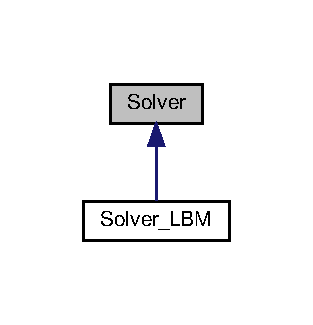
\includegraphics[width=150pt]{classSolver__inherit__graph}
\end{center}
\end{figure}


Collaboration diagram for Solver\+:
\nopagebreak
\begin{figure}[H]
\begin{center}
\leavevmode
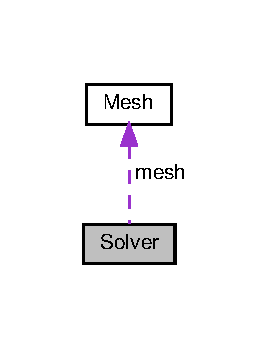
\includegraphics[width=130pt]{classSolver__coll__graph}
\end{center}
\end{figure}
\subsection*{Public Member Functions}
\begin{DoxyCompactItemize}
\item 
virtual int \hyperlink{classSolver_a354e0d709ec8c548be9e72add961c9f6}{S\+\_\+\+Init} ()=0
\item 
virtual int \hyperlink{classSolver_a52e834a160622462bec7c40054702270}{S\+\_\+\+Initialize} (int i\+\_\+dev, int L)=0
\item 
virtual int \hyperlink{classSolver_a4bbad207af5ea842a472a35049d4fbb9}{S\+\_\+\+Advance} (int i\+\_\+dev, int L, std\+::ofstream $\ast$file, double $\ast$tmp=0)=0
\item 
virtual int \hyperlink{classSolver_a28e21b098bfcf7c69a9664a8a4413960}{S\+\_\+\+Compute\+Ref\+Criteria} (int i\+\_\+dev, int L, int var)=0
\item 
virtual int \hyperlink{classSolver_a1b5b498836d6226bc425fb67bb7940d7}{S\+\_\+\+Evaluate\+Ref\+Criteria} (int i\+\_\+dev, int var)=0
\item 
virtual void \hyperlink{classSolver_a5b3e7308e48b43f75b09ddd425e11cfd}{S\+\_\+\+Interpolate} (int i\+\_\+dev, int L, int var)=0
\item 
virtual void \hyperlink{classSolver_a19b326267dbafa8b000b92a449c32b79}{S\+\_\+\+Average} (int i\+\_\+dev, int L, int var)=0
\item 
virtual void \hyperlink{classSolver_a8c73af137ee8c7ab25d8195448088a7b}{S\+\_\+\+Update\+Mesh} (int var, std\+::ofstream $\ast$file)=0
\item 
void \hyperlink{classSolver_a1ef012d41bd8d8f7f29fd15a8587dac9}{S\+\_\+\+Freeze\+Mesh} (int var)
\item 
\hyperlink{classSolver_a2608849f7c7dc3ec3e0c7b24e00712cf}{Solver} (\hyperlink{classMesh}{Mesh} $\ast$mesh\+\_\+)
\item 
\hyperlink{classSolver_aba52d3c92fafceb6fe39f937f2d73db3}{$\sim$\+Solver} ()
\end{DoxyCompactItemize}
\subsection*{Public Attributes}
\begin{DoxyCompactItemize}
\item 
\hyperlink{classMesh}{Mesh} $\ast$ \hyperlink{classSolver_a9b516765134fb4193329639761924cf7}{mesh}
\end{DoxyCompactItemize}


\subsection{Constructor \& Destructor Documentation}
\mbox{\Hypertarget{classSolver_a2608849f7c7dc3ec3e0c7b24e00712cf}\label{classSolver_a2608849f7c7dc3ec3e0c7b24e00712cf}} 
\index{Solver@{Solver}!Solver@{Solver}}
\index{Solver@{Solver}!Solver@{Solver}}
\subsubsection{\texorpdfstring{Solver()}{Solver()}}
{\footnotesize\ttfamily Solver\+::\+Solver (\begin{DoxyParamCaption}\item[{\hyperlink{classMesh}{Mesh} $\ast$}]{mesh\+\_\+ }\end{DoxyParamCaption})\hspace{0.3cm}{\ttfamily [inline]}}

\mbox{\Hypertarget{classSolver_aba52d3c92fafceb6fe39f937f2d73db3}\label{classSolver_aba52d3c92fafceb6fe39f937f2d73db3}} 
\index{Solver@{Solver}!````~Solver@{$\sim$\+Solver}}
\index{````~Solver@{$\sim$\+Solver}!Solver@{Solver}}
\subsubsection{\texorpdfstring{$\sim$\+Solver()}{~Solver()}}
{\footnotesize\ttfamily Solver\+::$\sim$\+Solver (\begin{DoxyParamCaption}{ }\end{DoxyParamCaption})\hspace{0.3cm}{\ttfamily [inline]}}



\subsection{Member Function Documentation}
\mbox{\Hypertarget{classSolver_a4bbad207af5ea842a472a35049d4fbb9}\label{classSolver_a4bbad207af5ea842a472a35049d4fbb9}} 
\index{Solver@{Solver}!S\+\_\+\+Advance@{S\+\_\+\+Advance}}
\index{S\+\_\+\+Advance@{S\+\_\+\+Advance}!Solver@{Solver}}
\subsubsection{\texorpdfstring{S\+\_\+\+Advance()}{S\_Advance()}}
{\footnotesize\ttfamily virtual int Solver\+::\+S\+\_\+\+Advance (\begin{DoxyParamCaption}\item[{int}]{i\+\_\+dev,  }\item[{int}]{L,  }\item[{std\+::ofstream $\ast$}]{file,  }\item[{double $\ast$}]{tmp = {\ttfamily 0} }\end{DoxyParamCaption})\hspace{0.3cm}{\ttfamily [pure virtual]}}



Implemented in \hyperlink{classSolver__LBM_a9f5927018c5068edc1f31ead745a6e05}{Solver\+\_\+\+L\+BM}.

\mbox{\Hypertarget{classSolver_a19b326267dbafa8b000b92a449c32b79}\label{classSolver_a19b326267dbafa8b000b92a449c32b79}} 
\index{Solver@{Solver}!S\+\_\+\+Average@{S\+\_\+\+Average}}
\index{S\+\_\+\+Average@{S\+\_\+\+Average}!Solver@{Solver}}
\subsubsection{\texorpdfstring{S\+\_\+\+Average()}{S\_Average()}}
{\footnotesize\ttfamily virtual void Solver\+::\+S\+\_\+\+Average (\begin{DoxyParamCaption}\item[{int}]{i\+\_\+dev,  }\item[{int}]{L,  }\item[{int}]{var }\end{DoxyParamCaption})\hspace{0.3cm}{\ttfamily [pure virtual]}}



Implemented in \hyperlink{classSolver__LBM_ae4487d21dd9b3f94a4e6e367b37698fa}{Solver\+\_\+\+L\+BM}.

\mbox{\Hypertarget{classSolver_a28e21b098bfcf7c69a9664a8a4413960}\label{classSolver_a28e21b098bfcf7c69a9664a8a4413960}} 
\index{Solver@{Solver}!S\+\_\+\+Compute\+Ref\+Criteria@{S\+\_\+\+Compute\+Ref\+Criteria}}
\index{S\+\_\+\+Compute\+Ref\+Criteria@{S\+\_\+\+Compute\+Ref\+Criteria}!Solver@{Solver}}
\subsubsection{\texorpdfstring{S\+\_\+\+Compute\+Ref\+Criteria()}{S\_ComputeRefCriteria()}}
{\footnotesize\ttfamily virtual int Solver\+::\+S\+\_\+\+Compute\+Ref\+Criteria (\begin{DoxyParamCaption}\item[{int}]{i\+\_\+dev,  }\item[{int}]{L,  }\item[{int}]{var }\end{DoxyParamCaption})\hspace{0.3cm}{\ttfamily [pure virtual]}}



Implemented in \hyperlink{classSolver__LBM_a9c7637ab5e8dde0e9c957661758a738e}{Solver\+\_\+\+L\+BM}.

\mbox{\Hypertarget{classSolver_a1b5b498836d6226bc425fb67bb7940d7}\label{classSolver_a1b5b498836d6226bc425fb67bb7940d7}} 
\index{Solver@{Solver}!S\+\_\+\+Evaluate\+Ref\+Criteria@{S\+\_\+\+Evaluate\+Ref\+Criteria}}
\index{S\+\_\+\+Evaluate\+Ref\+Criteria@{S\+\_\+\+Evaluate\+Ref\+Criteria}!Solver@{Solver}}
\subsubsection{\texorpdfstring{S\+\_\+\+Evaluate\+Ref\+Criteria()}{S\_EvaluateRefCriteria()}}
{\footnotesize\ttfamily virtual int Solver\+::\+S\+\_\+\+Evaluate\+Ref\+Criteria (\begin{DoxyParamCaption}\item[{int}]{i\+\_\+dev,  }\item[{int}]{var }\end{DoxyParamCaption})\hspace{0.3cm}{\ttfamily [pure virtual]}}



Implemented in \hyperlink{classSolver__LBM_a8809dbbf5653c40202da0611afb6dcaa}{Solver\+\_\+\+L\+BM}.

\mbox{\Hypertarget{classSolver_a1ef012d41bd8d8f7f29fd15a8587dac9}\label{classSolver_a1ef012d41bd8d8f7f29fd15a8587dac9}} 
\index{Solver@{Solver}!S\+\_\+\+Freeze\+Mesh@{S\+\_\+\+Freeze\+Mesh}}
\index{S\+\_\+\+Freeze\+Mesh@{S\+\_\+\+Freeze\+Mesh}!Solver@{Solver}}
\subsubsection{\texorpdfstring{S\+\_\+\+Freeze\+Mesh()}{S\_FreezeMesh()}}
{\footnotesize\ttfamily void Solver\+::\+S\+\_\+\+Freeze\+Mesh (\begin{DoxyParamCaption}\item[{int}]{var }\end{DoxyParamCaption})\hspace{0.3cm}{\ttfamily [inline]}}

\mbox{\Hypertarget{classSolver_a354e0d709ec8c548be9e72add961c9f6}\label{classSolver_a354e0d709ec8c548be9e72add961c9f6}} 
\index{Solver@{Solver}!S\+\_\+\+Init@{S\+\_\+\+Init}}
\index{S\+\_\+\+Init@{S\+\_\+\+Init}!Solver@{Solver}}
\subsubsection{\texorpdfstring{S\+\_\+\+Init()}{S\_Init()}}
{\footnotesize\ttfamily virtual int Solver\+::\+S\+\_\+\+Init (\begin{DoxyParamCaption}{ }\end{DoxyParamCaption})\hspace{0.3cm}{\ttfamily [pure virtual]}}



Implemented in \hyperlink{classSolver__LBM_ac8195f75a91e0c41f3b7908cebc5c8d6}{Solver\+\_\+\+L\+BM}.

\mbox{\Hypertarget{classSolver_a52e834a160622462bec7c40054702270}\label{classSolver_a52e834a160622462bec7c40054702270}} 
\index{Solver@{Solver}!S\+\_\+\+Initialize@{S\+\_\+\+Initialize}}
\index{S\+\_\+\+Initialize@{S\+\_\+\+Initialize}!Solver@{Solver}}
\subsubsection{\texorpdfstring{S\+\_\+\+Initialize()}{S\_Initialize()}}
{\footnotesize\ttfamily virtual int Solver\+::\+S\+\_\+\+Initialize (\begin{DoxyParamCaption}\item[{int}]{i\+\_\+dev,  }\item[{int}]{L }\end{DoxyParamCaption})\hspace{0.3cm}{\ttfamily [pure virtual]}}



Implemented in \hyperlink{classSolver__LBM_a215918c1e81dc85315651948bbc86173}{Solver\+\_\+\+L\+BM}.

\mbox{\Hypertarget{classSolver_a5b3e7308e48b43f75b09ddd425e11cfd}\label{classSolver_a5b3e7308e48b43f75b09ddd425e11cfd}} 
\index{Solver@{Solver}!S\+\_\+\+Interpolate@{S\+\_\+\+Interpolate}}
\index{S\+\_\+\+Interpolate@{S\+\_\+\+Interpolate}!Solver@{Solver}}
\subsubsection{\texorpdfstring{S\+\_\+\+Interpolate()}{S\_Interpolate()}}
{\footnotesize\ttfamily virtual void Solver\+::\+S\+\_\+\+Interpolate (\begin{DoxyParamCaption}\item[{int}]{i\+\_\+dev,  }\item[{int}]{L,  }\item[{int}]{var }\end{DoxyParamCaption})\hspace{0.3cm}{\ttfamily [pure virtual]}}



Implemented in \hyperlink{classSolver__LBM_a1ae0246ed9aa764eafce29a5f7ef7d42}{Solver\+\_\+\+L\+BM}.

\mbox{\Hypertarget{classSolver_a8c73af137ee8c7ab25d8195448088a7b}\label{classSolver_a8c73af137ee8c7ab25d8195448088a7b}} 
\index{Solver@{Solver}!S\+\_\+\+Update\+Mesh@{S\+\_\+\+Update\+Mesh}}
\index{S\+\_\+\+Update\+Mesh@{S\+\_\+\+Update\+Mesh}!Solver@{Solver}}
\subsubsection{\texorpdfstring{S\+\_\+\+Update\+Mesh()}{S\_UpdateMesh()}}
{\footnotesize\ttfamily virtual void Solver\+::\+S\+\_\+\+Update\+Mesh (\begin{DoxyParamCaption}\item[{int}]{var,  }\item[{std\+::ofstream $\ast$}]{file }\end{DoxyParamCaption})\hspace{0.3cm}{\ttfamily [pure virtual]}}



Implemented in \hyperlink{classSolver__LBM_a59e8d7c94e3895a3586972bdbf0ebb77}{Solver\+\_\+\+L\+BM}.



\subsection{Member Data Documentation}
\mbox{\Hypertarget{classSolver_a9b516765134fb4193329639761924cf7}\label{classSolver_a9b516765134fb4193329639761924cf7}} 
\index{Solver@{Solver}!mesh@{mesh}}
\index{mesh@{mesh}!Solver@{Solver}}
\subsubsection{\texorpdfstring{mesh}{mesh}}
{\footnotesize\ttfamily \hyperlink{classMesh}{Mesh}$\ast$ Solver\+::mesh}



The documentation for this class was generated from the following file\+:\begin{DoxyCompactItemize}
\item 
inc/\hyperlink{solver_8h}{solver.\+h}\end{DoxyCompactItemize}

\hypertarget{classSolver__LBM}{}\section{Solver\+\_\+\+L\+BM Class Reference}
\label{classSolver__LBM}\index{Solver\+\_\+\+L\+BM@{Solver\+\_\+\+L\+BM}}


{\ttfamily \#include $<$solver.\+h$>$}



Inheritance diagram for Solver\+\_\+\+L\+BM\+:
\nopagebreak
\begin{figure}[H]
\begin{center}
\leavevmode
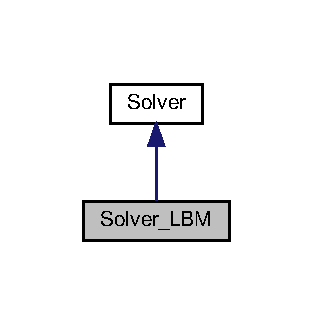
\includegraphics[width=150pt]{classSolver__LBM__inherit__graph}
\end{center}
\end{figure}


Collaboration diagram for Solver\+\_\+\+L\+BM\+:
\nopagebreak
\begin{figure}[H]
\begin{center}
\leavevmode
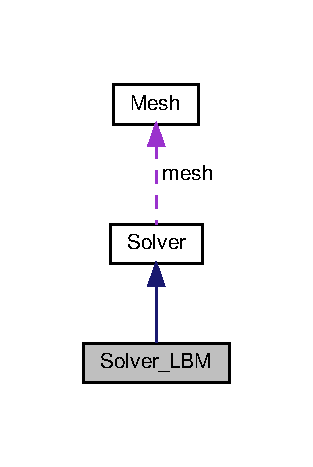
\includegraphics[width=150pt]{classSolver__LBM__coll__graph}
\end{center}
\end{figure}
\subsection*{Public Member Functions}
\begin{DoxyCompactItemize}
\item 
int \hyperlink{classSolver__LBM_abf91dd13737bd2232d191e21c20cbc33}{S\+\_\+\+Set\+Values\+Debug} (int i\+\_\+dev, int L, \hyperlink{cppspec_8h_af529d360dfac9b9578aa719418a53a21}{ufloat\+\_\+t} v)
\item 
int \hyperlink{classSolver__LBM_a05326a4c80d68bd0f7e70186fb8c4c38}{S\+\_\+\+Set\+Initial\+Conditions} (int i\+\_\+dev, int L, bool init)
\item 
int \hyperlink{classSolver__LBM_ac172ea0929788514a72ee6b42befe84c}{S\+\_\+\+ComputeU} (int i\+\_\+dev, int L)
\item 
int \hyperlink{classSolver__LBM_a9d31d1d8602462a3134a320c9e3d7c2c}{S\+\_\+\+ComputeW} (int i\+\_\+dev, int L)
\item 
int \hyperlink{classSolver__LBM_ab8c4daacb227f1ac1bf6a54097d65bd3}{S\+\_\+\+Collide} (int i\+\_\+dev, int L)
\item 
int \hyperlink{classSolver__LBM_ad301e7ccad5f700a94a12762f92939db}{S\+\_\+\+Stream} (int i\+\_\+dev, int L)
\item 
int \hyperlink{classSolver__LBM_acacdadaa96b72ca8a7f13a657a25c6f1}{S\+\_\+\+Compute\+Eq} (int i\+\_\+dev, int L)
\item 
void \hyperlink{classSolver__LBM_a1ae0246ed9aa764eafce29a5f7ef7d42}{S\+\_\+\+Interpolate} (int i\+\_\+dev, int L, int var)
\item 
void \hyperlink{classSolver__LBM_ae4487d21dd9b3f94a4e6e367b37698fa}{S\+\_\+\+Average} (int i\+\_\+dev, int L, int var)
\item 
int \hyperlink{classSolver__LBM_ac8195f75a91e0c41f3b7908cebc5c8d6}{S\+\_\+\+Init} ()
\item 
int \hyperlink{classSolver__LBM_a215918c1e81dc85315651948bbc86173}{S\+\_\+\+Initialize} (int i\+\_\+dev, int L)
\item 
int \hyperlink{classSolver__LBM_a9f5927018c5068edc1f31ead745a6e05}{S\+\_\+\+Advance} (int i\+\_\+dev, int L, std\+::ofstream $\ast$file, double $\ast$tmp=0)
\item 
int \hyperlink{classSolver__LBM_a9c7637ab5e8dde0e9c957661758a738e}{S\+\_\+\+Compute\+Ref\+Criteria} (int i\+\_\+dev, int L, int var)
\item 
int \hyperlink{classSolver__LBM_a8809dbbf5653c40202da0611afb6dcaa}{S\+\_\+\+Evaluate\+Ref\+Criteria} (int i\+\_\+dev, int var)
\item 
void \hyperlink{classSolver__LBM_a59e8d7c94e3895a3586972bdbf0ebb77}{S\+\_\+\+Update\+Mesh} (int var, std\+::ofstream $\ast$file)
\item 
\hyperlink{classSolver__LBM_a8fed041efa5cee6ff2eaba9c23406074}{Solver\+\_\+\+L\+BM} (\hyperlink{classMesh}{Mesh} $\ast$\hyperlink{classSolver_a9b516765134fb4193329639761924cf7}{mesh})
\end{DoxyCompactItemize}
\subsection*{Private Attributes}
\begin{DoxyCompactItemize}
\item 
\hyperlink{cppspec_8h_af529d360dfac9b9578aa719418a53a21}{ufloat\+\_\+t} \hyperlink{classSolver__LBM_a1ece0e58740be29fcaea526f7da7fe4a}{dx\+\_\+vec} \mbox{[}\hyperlink{cppspec_8h_add784659439a8dd6b1423406171414d3}{M\+A\+X\+\_\+\+L\+E\+V\+E\+LS}\mbox{]}
\item 
\hyperlink{cppspec_8h_af529d360dfac9b9578aa719418a53a21}{ufloat\+\_\+t} \hyperlink{classSolver__LBM_ad5b36057b2d1db724ff10f4dd6b59105}{tau\+\_\+vec} \mbox{[}\hyperlink{cppspec_8h_add784659439a8dd6b1423406171414d3}{M\+A\+X\+\_\+\+L\+E\+V\+E\+LS}\mbox{]}
\end{DoxyCompactItemize}
\subsection*{Additional Inherited Members}


\subsection{Constructor \& Destructor Documentation}
\mbox{\Hypertarget{classSolver__LBM_a8fed041efa5cee6ff2eaba9c23406074}\label{classSolver__LBM_a8fed041efa5cee6ff2eaba9c23406074}} 
\index{Solver\+\_\+\+L\+BM@{Solver\+\_\+\+L\+BM}!Solver\+\_\+\+L\+BM@{Solver\+\_\+\+L\+BM}}
\index{Solver\+\_\+\+L\+BM@{Solver\+\_\+\+L\+BM}!Solver\+\_\+\+L\+BM@{Solver\+\_\+\+L\+BM}}
\subsubsection{\texorpdfstring{Solver\+\_\+\+L\+B\+M()}{Solver\_LBM()}}
{\footnotesize\ttfamily Solver\+\_\+\+L\+B\+M\+::\+Solver\+\_\+\+L\+BM (\begin{DoxyParamCaption}\item[{\hyperlink{classMesh}{Mesh} $\ast$}]{mesh }\end{DoxyParamCaption})\hspace{0.3cm}{\ttfamily [inline]}}



\subsection{Member Function Documentation}
\mbox{\Hypertarget{classSolver__LBM_a9f5927018c5068edc1f31ead745a6e05}\label{classSolver__LBM_a9f5927018c5068edc1f31ead745a6e05}} 
\index{Solver\+\_\+\+L\+BM@{Solver\+\_\+\+L\+BM}!S\+\_\+\+Advance@{S\+\_\+\+Advance}}
\index{S\+\_\+\+Advance@{S\+\_\+\+Advance}!Solver\+\_\+\+L\+BM@{Solver\+\_\+\+L\+BM}}
\subsubsection{\texorpdfstring{S\+\_\+\+Advance()}{S\_Advance()}}
{\footnotesize\ttfamily int Solver\+\_\+\+L\+B\+M\+::\+S\+\_\+\+Advance (\begin{DoxyParamCaption}\item[{int}]{i\+\_\+dev,  }\item[{int}]{L,  }\item[{std\+::ofstream $\ast$}]{file,  }\item[{double $\ast$}]{tmp = {\ttfamily 0} }\end{DoxyParamCaption})\hspace{0.3cm}{\ttfamily [virtual]}}



Implements \hyperlink{classSolver_a4bbad207af5ea842a472a35049d4fbb9}{Solver}.

\mbox{\Hypertarget{classSolver__LBM_ae4487d21dd9b3f94a4e6e367b37698fa}\label{classSolver__LBM_ae4487d21dd9b3f94a4e6e367b37698fa}} 
\index{Solver\+\_\+\+L\+BM@{Solver\+\_\+\+L\+BM}!S\+\_\+\+Average@{S\+\_\+\+Average}}
\index{S\+\_\+\+Average@{S\+\_\+\+Average}!Solver\+\_\+\+L\+BM@{Solver\+\_\+\+L\+BM}}
\subsubsection{\texorpdfstring{S\+\_\+\+Average()}{S\_Average()}}
{\footnotesize\ttfamily void Solver\+\_\+\+L\+B\+M\+::\+S\+\_\+\+Average (\begin{DoxyParamCaption}\item[{int}]{i\+\_\+dev,  }\item[{int}]{L,  }\item[{int}]{var }\end{DoxyParamCaption})\hspace{0.3cm}{\ttfamily [inline]}, {\ttfamily [virtual]}}



Implements \hyperlink{classSolver_a19b326267dbafa8b000b92a449c32b79}{Solver}.

\mbox{\Hypertarget{classSolver__LBM_ab8c4daacb227f1ac1bf6a54097d65bd3}\label{classSolver__LBM_ab8c4daacb227f1ac1bf6a54097d65bd3}} 
\index{Solver\+\_\+\+L\+BM@{Solver\+\_\+\+L\+BM}!S\+\_\+\+Collide@{S\+\_\+\+Collide}}
\index{S\+\_\+\+Collide@{S\+\_\+\+Collide}!Solver\+\_\+\+L\+BM@{Solver\+\_\+\+L\+BM}}
\subsubsection{\texorpdfstring{S\+\_\+\+Collide()}{S\_Collide()}}
{\footnotesize\ttfamily int Solver\+\_\+\+L\+B\+M\+::\+S\+\_\+\+Collide (\begin{DoxyParamCaption}\item[{int}]{i\+\_\+dev,  }\item[{int}]{L }\end{DoxyParamCaption})}

\mbox{\Hypertarget{classSolver__LBM_acacdadaa96b72ca8a7f13a657a25c6f1}\label{classSolver__LBM_acacdadaa96b72ca8a7f13a657a25c6f1}} 
\index{Solver\+\_\+\+L\+BM@{Solver\+\_\+\+L\+BM}!S\+\_\+\+Compute\+Eq@{S\+\_\+\+Compute\+Eq}}
\index{S\+\_\+\+Compute\+Eq@{S\+\_\+\+Compute\+Eq}!Solver\+\_\+\+L\+BM@{Solver\+\_\+\+L\+BM}}
\subsubsection{\texorpdfstring{S\+\_\+\+Compute\+Eq()}{S\_ComputeEq()}}
{\footnotesize\ttfamily int Solver\+\_\+\+L\+B\+M\+::\+S\+\_\+\+Compute\+Eq (\begin{DoxyParamCaption}\item[{int}]{i\+\_\+dev,  }\item[{int}]{L }\end{DoxyParamCaption})}

\mbox{\Hypertarget{classSolver__LBM_a9c7637ab5e8dde0e9c957661758a738e}\label{classSolver__LBM_a9c7637ab5e8dde0e9c957661758a738e}} 
\index{Solver\+\_\+\+L\+BM@{Solver\+\_\+\+L\+BM}!S\+\_\+\+Compute\+Ref\+Criteria@{S\+\_\+\+Compute\+Ref\+Criteria}}
\index{S\+\_\+\+Compute\+Ref\+Criteria@{S\+\_\+\+Compute\+Ref\+Criteria}!Solver\+\_\+\+L\+BM@{Solver\+\_\+\+L\+BM}}
\subsubsection{\texorpdfstring{S\+\_\+\+Compute\+Ref\+Criteria()}{S\_ComputeRefCriteria()}}
{\footnotesize\ttfamily int Solver\+\_\+\+L\+B\+M\+::\+S\+\_\+\+Compute\+Ref\+Criteria (\begin{DoxyParamCaption}\item[{int}]{i\+\_\+dev,  }\item[{int}]{L,  }\item[{int}]{var }\end{DoxyParamCaption})\hspace{0.3cm}{\ttfamily [virtual]}}



Implements \hyperlink{classSolver_a28e21b098bfcf7c69a9664a8a4413960}{Solver}.

\mbox{\Hypertarget{classSolver__LBM_ac172ea0929788514a72ee6b42befe84c}\label{classSolver__LBM_ac172ea0929788514a72ee6b42befe84c}} 
\index{Solver\+\_\+\+L\+BM@{Solver\+\_\+\+L\+BM}!S\+\_\+\+ComputeU@{S\+\_\+\+ComputeU}}
\index{S\+\_\+\+ComputeU@{S\+\_\+\+ComputeU}!Solver\+\_\+\+L\+BM@{Solver\+\_\+\+L\+BM}}
\subsubsection{\texorpdfstring{S\+\_\+\+Compute\+U()}{S\_ComputeU()}}
{\footnotesize\ttfamily int Solver\+\_\+\+L\+B\+M\+::\+S\+\_\+\+ComputeU (\begin{DoxyParamCaption}\item[{int}]{i\+\_\+dev,  }\item[{int}]{L }\end{DoxyParamCaption})}

\mbox{\Hypertarget{classSolver__LBM_a9d31d1d8602462a3134a320c9e3d7c2c}\label{classSolver__LBM_a9d31d1d8602462a3134a320c9e3d7c2c}} 
\index{Solver\+\_\+\+L\+BM@{Solver\+\_\+\+L\+BM}!S\+\_\+\+ComputeW@{S\+\_\+\+ComputeW}}
\index{S\+\_\+\+ComputeW@{S\+\_\+\+ComputeW}!Solver\+\_\+\+L\+BM@{Solver\+\_\+\+L\+BM}}
\subsubsection{\texorpdfstring{S\+\_\+\+Compute\+W()}{S\_ComputeW()}}
{\footnotesize\ttfamily int Solver\+\_\+\+L\+B\+M\+::\+S\+\_\+\+ComputeW (\begin{DoxyParamCaption}\item[{int}]{i\+\_\+dev,  }\item[{int}]{L }\end{DoxyParamCaption})}

\mbox{\Hypertarget{classSolver__LBM_a8809dbbf5653c40202da0611afb6dcaa}\label{classSolver__LBM_a8809dbbf5653c40202da0611afb6dcaa}} 
\index{Solver\+\_\+\+L\+BM@{Solver\+\_\+\+L\+BM}!S\+\_\+\+Evaluate\+Ref\+Criteria@{S\+\_\+\+Evaluate\+Ref\+Criteria}}
\index{S\+\_\+\+Evaluate\+Ref\+Criteria@{S\+\_\+\+Evaluate\+Ref\+Criteria}!Solver\+\_\+\+L\+BM@{Solver\+\_\+\+L\+BM}}
\subsubsection{\texorpdfstring{S\+\_\+\+Evaluate\+Ref\+Criteria()}{S\_EvaluateRefCriteria()}}
{\footnotesize\ttfamily int Solver\+\_\+\+L\+B\+M\+::\+S\+\_\+\+Evaluate\+Ref\+Criteria (\begin{DoxyParamCaption}\item[{int}]{i\+\_\+dev,  }\item[{int}]{var }\end{DoxyParamCaption})\hspace{0.3cm}{\ttfamily [virtual]}}



Implements \hyperlink{classSolver_a1b5b498836d6226bc425fb67bb7940d7}{Solver}.

\mbox{\Hypertarget{classSolver__LBM_ac8195f75a91e0c41f3b7908cebc5c8d6}\label{classSolver__LBM_ac8195f75a91e0c41f3b7908cebc5c8d6}} 
\index{Solver\+\_\+\+L\+BM@{Solver\+\_\+\+L\+BM}!S\+\_\+\+Init@{S\+\_\+\+Init}}
\index{S\+\_\+\+Init@{S\+\_\+\+Init}!Solver\+\_\+\+L\+BM@{Solver\+\_\+\+L\+BM}}
\subsubsection{\texorpdfstring{S\+\_\+\+Init()}{S\_Init()}}
{\footnotesize\ttfamily int Solver\+\_\+\+L\+B\+M\+::\+S\+\_\+\+Init (\begin{DoxyParamCaption}{ }\end{DoxyParamCaption})\hspace{0.3cm}{\ttfamily [virtual]}}



Implements \hyperlink{classSolver_a354e0d709ec8c548be9e72add961c9f6}{Solver}.

\mbox{\Hypertarget{classSolver__LBM_a215918c1e81dc85315651948bbc86173}\label{classSolver__LBM_a215918c1e81dc85315651948bbc86173}} 
\index{Solver\+\_\+\+L\+BM@{Solver\+\_\+\+L\+BM}!S\+\_\+\+Initialize@{S\+\_\+\+Initialize}}
\index{S\+\_\+\+Initialize@{S\+\_\+\+Initialize}!Solver\+\_\+\+L\+BM@{Solver\+\_\+\+L\+BM}}
\subsubsection{\texorpdfstring{S\+\_\+\+Initialize()}{S\_Initialize()}}
{\footnotesize\ttfamily int Solver\+\_\+\+L\+B\+M\+::\+S\+\_\+\+Initialize (\begin{DoxyParamCaption}\item[{int}]{i\+\_\+dev,  }\item[{int}]{L }\end{DoxyParamCaption})\hspace{0.3cm}{\ttfamily [virtual]}}



Implements \hyperlink{classSolver_a52e834a160622462bec7c40054702270}{Solver}.

\mbox{\Hypertarget{classSolver__LBM_a1ae0246ed9aa764eafce29a5f7ef7d42}\label{classSolver__LBM_a1ae0246ed9aa764eafce29a5f7ef7d42}} 
\index{Solver\+\_\+\+L\+BM@{Solver\+\_\+\+L\+BM}!S\+\_\+\+Interpolate@{S\+\_\+\+Interpolate}}
\index{S\+\_\+\+Interpolate@{S\+\_\+\+Interpolate}!Solver\+\_\+\+L\+BM@{Solver\+\_\+\+L\+BM}}
\subsubsection{\texorpdfstring{S\+\_\+\+Interpolate()}{S\_Interpolate()}}
{\footnotesize\ttfamily void Solver\+\_\+\+L\+B\+M\+::\+S\+\_\+\+Interpolate (\begin{DoxyParamCaption}\item[{int}]{i\+\_\+dev,  }\item[{int}]{L,  }\item[{int}]{var }\end{DoxyParamCaption})\hspace{0.3cm}{\ttfamily [inline]}, {\ttfamily [virtual]}}



Implements \hyperlink{classSolver_a5b3e7308e48b43f75b09ddd425e11cfd}{Solver}.

\mbox{\Hypertarget{classSolver__LBM_a05326a4c80d68bd0f7e70186fb8c4c38}\label{classSolver__LBM_a05326a4c80d68bd0f7e70186fb8c4c38}} 
\index{Solver\+\_\+\+L\+BM@{Solver\+\_\+\+L\+BM}!S\+\_\+\+Set\+Initial\+Conditions@{S\+\_\+\+Set\+Initial\+Conditions}}
\index{S\+\_\+\+Set\+Initial\+Conditions@{S\+\_\+\+Set\+Initial\+Conditions}!Solver\+\_\+\+L\+BM@{Solver\+\_\+\+L\+BM}}
\subsubsection{\texorpdfstring{S\+\_\+\+Set\+Initial\+Conditions()}{S\_SetInitialConditions()}}
{\footnotesize\ttfamily int Solver\+\_\+\+L\+B\+M\+::\+S\+\_\+\+Set\+Initial\+Conditions (\begin{DoxyParamCaption}\item[{int}]{i\+\_\+dev,  }\item[{int}]{L,  }\item[{bool}]{init }\end{DoxyParamCaption})}

\mbox{\Hypertarget{classSolver__LBM_abf91dd13737bd2232d191e21c20cbc33}\label{classSolver__LBM_abf91dd13737bd2232d191e21c20cbc33}} 
\index{Solver\+\_\+\+L\+BM@{Solver\+\_\+\+L\+BM}!S\+\_\+\+Set\+Values\+Debug@{S\+\_\+\+Set\+Values\+Debug}}
\index{S\+\_\+\+Set\+Values\+Debug@{S\+\_\+\+Set\+Values\+Debug}!Solver\+\_\+\+L\+BM@{Solver\+\_\+\+L\+BM}}
\subsubsection{\texorpdfstring{S\+\_\+\+Set\+Values\+Debug()}{S\_SetValuesDebug()}}
{\footnotesize\ttfamily int Solver\+\_\+\+L\+B\+M\+::\+S\+\_\+\+Set\+Values\+Debug (\begin{DoxyParamCaption}\item[{int}]{i\+\_\+dev,  }\item[{int}]{L,  }\item[{\hyperlink{cppspec_8h_af529d360dfac9b9578aa719418a53a21}{ufloat\+\_\+t}}]{v }\end{DoxyParamCaption})}

\mbox{\Hypertarget{classSolver__LBM_ad301e7ccad5f700a94a12762f92939db}\label{classSolver__LBM_ad301e7ccad5f700a94a12762f92939db}} 
\index{Solver\+\_\+\+L\+BM@{Solver\+\_\+\+L\+BM}!S\+\_\+\+Stream@{S\+\_\+\+Stream}}
\index{S\+\_\+\+Stream@{S\+\_\+\+Stream}!Solver\+\_\+\+L\+BM@{Solver\+\_\+\+L\+BM}}
\subsubsection{\texorpdfstring{S\+\_\+\+Stream()}{S\_Stream()}}
{\footnotesize\ttfamily int Solver\+\_\+\+L\+B\+M\+::\+S\+\_\+\+Stream (\begin{DoxyParamCaption}\item[{int}]{i\+\_\+dev,  }\item[{int}]{L }\end{DoxyParamCaption})}

\mbox{\Hypertarget{classSolver__LBM_a59e8d7c94e3895a3586972bdbf0ebb77}\label{classSolver__LBM_a59e8d7c94e3895a3586972bdbf0ebb77}} 
\index{Solver\+\_\+\+L\+BM@{Solver\+\_\+\+L\+BM}!S\+\_\+\+Update\+Mesh@{S\+\_\+\+Update\+Mesh}}
\index{S\+\_\+\+Update\+Mesh@{S\+\_\+\+Update\+Mesh}!Solver\+\_\+\+L\+BM@{Solver\+\_\+\+L\+BM}}
\subsubsection{\texorpdfstring{S\+\_\+\+Update\+Mesh()}{S\_UpdateMesh()}}
{\footnotesize\ttfamily void Solver\+\_\+\+L\+B\+M\+::\+S\+\_\+\+Update\+Mesh (\begin{DoxyParamCaption}\item[{int}]{var,  }\item[{std\+::ofstream $\ast$}]{file }\end{DoxyParamCaption})\hspace{0.3cm}{\ttfamily [inline]}, {\ttfamily [virtual]}}



Implements \hyperlink{classSolver_a8c73af137ee8c7ab25d8195448088a7b}{Solver}.



\subsection{Member Data Documentation}
\mbox{\Hypertarget{classSolver__LBM_a1ece0e58740be29fcaea526f7da7fe4a}\label{classSolver__LBM_a1ece0e58740be29fcaea526f7da7fe4a}} 
\index{Solver\+\_\+\+L\+BM@{Solver\+\_\+\+L\+BM}!dx\+\_\+vec@{dx\+\_\+vec}}
\index{dx\+\_\+vec@{dx\+\_\+vec}!Solver\+\_\+\+L\+BM@{Solver\+\_\+\+L\+BM}}
\subsubsection{\texorpdfstring{dx\+\_\+vec}{dx\_vec}}
{\footnotesize\ttfamily \hyperlink{cppspec_8h_af529d360dfac9b9578aa719418a53a21}{ufloat\+\_\+t} Solver\+\_\+\+L\+B\+M\+::dx\+\_\+vec\mbox{[}\hyperlink{cppspec_8h_add784659439a8dd6b1423406171414d3}{M\+A\+X\+\_\+\+L\+E\+V\+E\+LS}\mbox{]}\hspace{0.3cm}{\ttfamily [private]}}

\mbox{\Hypertarget{classSolver__LBM_ad5b36057b2d1db724ff10f4dd6b59105}\label{classSolver__LBM_ad5b36057b2d1db724ff10f4dd6b59105}} 
\index{Solver\+\_\+\+L\+BM@{Solver\+\_\+\+L\+BM}!tau\+\_\+vec@{tau\+\_\+vec}}
\index{tau\+\_\+vec@{tau\+\_\+vec}!Solver\+\_\+\+L\+BM@{Solver\+\_\+\+L\+BM}}
\subsubsection{\texorpdfstring{tau\+\_\+vec}{tau\_vec}}
{\footnotesize\ttfamily \hyperlink{cppspec_8h_af529d360dfac9b9578aa719418a53a21}{ufloat\+\_\+t} Solver\+\_\+\+L\+B\+M\+::tau\+\_\+vec\mbox{[}\hyperlink{cppspec_8h_add784659439a8dd6b1423406171414d3}{M\+A\+X\+\_\+\+L\+E\+V\+E\+LS}\mbox{]}\hspace{0.3cm}{\ttfamily [private]}}



The documentation for this class was generated from the following file\+:\begin{DoxyCompactItemize}
\item 
inc/\hyperlink{solver_8h}{solver.\+h}\end{DoxyCompactItemize}

\chapter{File Documentation}
\hypertarget{cppspec_8h}{}\section{inc/cppspec.h File Reference}
\label{cppspec_8h}\index{inc/cppspec.\+h@{inc/cppspec.\+h}}
{\ttfamily \#include $<$iostream$>$}\newline
{\ttfamily \#include $<$fstream$>$}\newline
{\ttfamily \#include $<$vector$>$}\newline
{\ttfamily \#include $<$math.\+h$>$}\newline
{\ttfamily \#include $<$ctime$>$}\newline
{\ttfamily \#include $<$chrono$>$}\newline
{\ttfamily \#include $<$thread$>$}\newline
{\ttfamily \#include $<$unistd.\+h$>$}\newline
{\ttfamily \#include $<$algorithm$>$}\newline
{\ttfamily \#include $<$random$>$}\newline
{\ttfamily \#include $<$thrust/host\+\_\+vector.\+h$>$}\newline
{\ttfamily \#include $<$thrust/device\+\_\+ptr.\+h$>$}\newline
{\ttfamily \#include $<$thrust/extrema.\+h$>$}\newline
{\ttfamily \#include $<$thrust/execution\+\_\+policy.\+h$>$}\newline
{\ttfamily \#include $<$thrust/iterator/counting\+\_\+iterator.\+h$>$}\newline
{\ttfamily \#include $<$thrust/gather.\+h$>$}\newline
{\ttfamily \#include \char`\"{}vtk\+A\+M\+R\+Box.\+h\char`\"{}}\newline
{\ttfamily \#include \char`\"{}vtk\+A\+M\+R\+Utilities.\+h\char`\"{}}\newline
{\ttfamily \#include \char`\"{}vtk\+Cell.\+h\char`\"{}}\newline
{\ttfamily \#include \char`\"{}vtk\+Cell\+Data.\+h\char`\"{}}\newline
{\ttfamily \#include \char`\"{}vtk\+Composite\+Data\+Writer.\+h\char`\"{}}\newline
{\ttfamily \#include \char`\"{}vtk\+Data\+Array.\+h\char`\"{}}\newline
{\ttfamily \#include \char`\"{}vtk\+Double\+Array.\+h\char`\"{}}\newline
{\ttfamily \#include \char`\"{}vtk\+Multi\+Block\+Data\+Set.\+h\char`\"{}}\newline
{\ttfamily \#include \char`\"{}vtk\+New.\+h\char`\"{}}\newline
{\ttfamily \#include \char`\"{}vtk\+Overlapping\+A\+M\+R.\+h\char`\"{}}\newline
{\ttfamily \#include \char`\"{}vtk\+Point\+Data.\+h\char`\"{}}\newline
{\ttfamily \#include \char`\"{}vtk\+Points.\+h\char`\"{}}\newline
{\ttfamily \#include \char`\"{}vtk\+Uniform\+Grid.\+h\char`\"{}}\newline
{\ttfamily \#include \char`\"{}vtk\+X\+M\+L\+Image\+Data\+Writer.\+h\char`\"{}}\newline
{\ttfamily \#include \char`\"{}vtk\+X\+M\+L\+Multi\+Block\+Data\+Writer.\+h\char`\"{}}\newline
{\ttfamily \#include \char`\"{}vtk\+X\+M\+L\+Uniform\+Grid\+A\+M\+R\+Reader.\+h\char`\"{}}\newline
{\ttfamily \#include \char`\"{}vtk\+Unstructured\+Grid.\+h\char`\"{}}\newline
{\ttfamily \#include \char`\"{}vtk\+X\+M\+L\+Hierarchical\+Box\+Data\+Writer.\+h\char`\"{}}\newline
{\ttfamily \#include \char`\"{}vtk\+X\+M\+L\+Uniform\+Grid\+A\+M\+R\+Writer.\+h\char`\"{}}\newline
Include dependency graph for cppspec.\+h\+:
\nopagebreak
\begin{figure}[H]
\begin{center}
\leavevmode
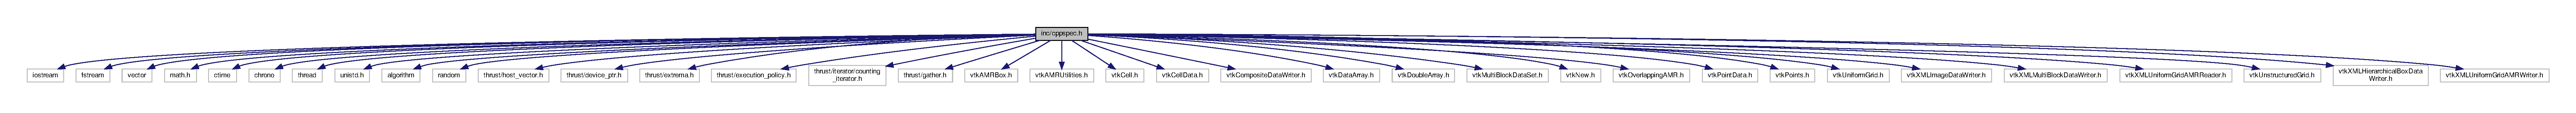
\includegraphics[width=350pt]{cppspec_8h__incl}
\end{center}
\end{figure}
This graph shows which files directly or indirectly include this file\+:
\nopagebreak
\begin{figure}[H]
\begin{center}
\leavevmode
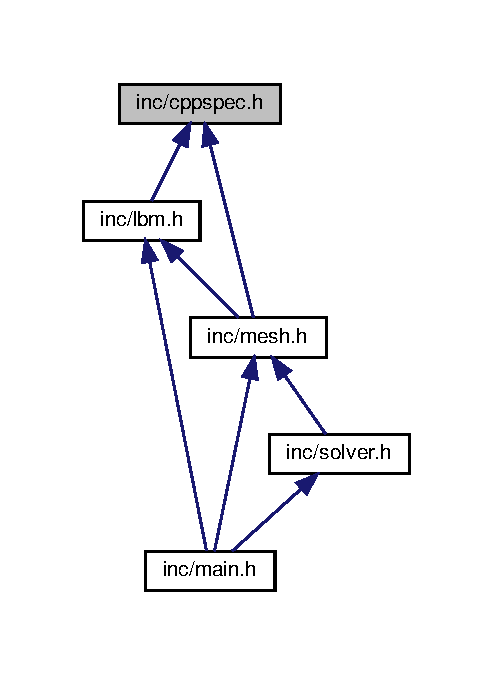
\includegraphics[width=237pt]{cppspec_8h__dep__incl}
\end{center}
\end{figure}
\subsection*{Macros}
\begin{DoxyCompactItemize}
\item 
\#define \hyperlink{cppspec_8h_a471e2491cf3df4197fe5b39387103e8e}{N\+\_\+\+P\+R\+E\+C\+I\+S\+I\+ON}~0
\begin{DoxyCompactList}\small\item\em Floating-\/point precision for data storage. \end{DoxyCompactList}\item 
\#define \hyperlink{cppspec_8h_a327d0faa306d7663502be8df312a815e}{N\+\_\+\+D\+IM}~3
\begin{DoxyCompactList}\small\item\em Number of dimensions. \end{DoxyCompactList}\item 
\#define \hyperlink{cppspec_8h_add784659439a8dd6b1423406171414d3}{M\+A\+X\+\_\+\+L\+E\+V\+E\+LS}~3
\begin{DoxyCompactList}\small\item\em Maximum number of levels in the grid hierarchy. \end{DoxyCompactList}\item 
\#define \hyperlink{cppspec_8h_a42f8c497a1968074f38bf5055c650dca}{V\+E\+R\+B\+O\+SE}~0
\begin{DoxyCompactList}\small\item\em Controls level of output reporting. \end{DoxyCompactList}\item 
\#define \hyperlink{cppspec_8h_aa5f8c50e07266a952522f228d6a79399}{S\+\_\+\+L\+ES}~0
\begin{DoxyCompactList}\small\item\em Indicator for applying Smagorinsky subgrid-\/scale modeling. \end{DoxyCompactList}\item 
\#define \hyperlink{cppspec_8h_a0d2c963c4479bfcef9727d6481a0b784}{S\+\_\+\+T\+Y\+PE}~1
\begin{DoxyCompactList}\small\item\em Controls streaming type for Lattice Boltzmann solver. \end{DoxyCompactList}\item 
\#define \hyperlink{cppspec_8h_ac8269dbb8d792c70ffed77d1e0dbdd31}{P\+\_\+\+D\+I\+R\+\_\+\+N\+A\+ME}~\char`\"{}../out/results/\char`\"{}
\item 
\#define \hyperlink{cppspec_8h_a1d65ef6030322ded390e1b8881dd1139}{N\+\_\+\+D\+I\+Mc}~(\hyperlink{cppspec_8h_a327d0faa306d7663502be8df312a815e}{N\+\_\+\+D\+IM}-\/2)
\item 
\#define \hyperlink{cppspec_8h_a02807d71c48e98f5c48f1697ae92b542}{N\+\_\+U}~(1+\hyperlink{cppspec_8h_a327d0faa306d7663502be8df312a815e}{N\+\_\+\+D\+IM})
\item 
\#define \hyperlink{cppspec_8h_ae7141a84f3fe0ddcd628a6d8ee0a4ea8}{N\+\_\+\+S\+K\+I\+P\+ID}~-\/999
\item 
\#define \hyperlink{cppspec_8h_a445b3d4fd28972a4c8050fa6b7f4df6e}{A\+P\+P\+E\+ND}(x,  y)~x \#\# y
\item 
\#define \hyperlink{cppspec_8h_af18a56c205ea2070bee498a5e17156b8}{N\+\_\+\+Pf}(x)~(\hyperlink{cppspec_8h_a445b3d4fd28972a4c8050fa6b7f4df6e}{A\+P\+P\+E\+ND}(x,F))
\item 
\#define \hyperlink{cppspec_8h_a39646502414a17a8518d029263259eee}{N\+\_\+\+C\+H\+I\+L\+D\+R\+EN}~8
\item 
\#define \hyperlink{cppspec_8h_a58f5ae3b2b4bb74f9f710b74270d6f9e}{Nbx}~4
\item 
\#define \hyperlink{cppspec_8h_a0c0bb72cd8b2c5622f7ceb36d730770f}{M\+\_\+\+C\+B\+L\+O\+CK}~64
\item 
\#define \hyperlink{cppspec_8h_a2b674dab7a14f1bf32b48b7fda5022dc}{N\+\_\+\+D\+EV}~1
\begin{DoxyCompactList}\small\item\em Number of G\+PU devices to employ. \end{DoxyCompactList}\item 
\#define \hyperlink{cppspec_8h_a4c7e3fe601ae8091af0b966332bf7878}{M\+\_\+\+B\+L\+O\+CK}~128
\begin{DoxyCompactList}\small\item\em Numer of threads per thread-\/block. \end{DoxyCompactList}\item 
\#define \hyperlink{cppspec_8h_a7ad2aa54e5126c6493cb64144e693537}{M\+\_\+maxcells\+\_\+roundoff}~2048
\begin{DoxyCompactList}\small\item\em Round-\/off parameter for computation of n\+\_\+maxcells. \end{DoxyCompactList}\item 
\#define \hyperlink{cppspec_8h_af093d941bc37a7a3f38e1db6593d9633}{Nx}~64
\item 
\#define \hyperlink{cppspec_8h_ab6471b0dc18a88669e137a1223f9cad8}{Nx2}~(\hyperlink{cppspec_8h_af093d941bc37a7a3f38e1db6593d9633}{Nx}$\ast$\hyperlink{cppspec_8h_af093d941bc37a7a3f38e1db6593d9633}{Nx})
\item 
\#define \hyperlink{cppspec_8h_a46b57ac64aa41628a8acc88e9b8d7e4f}{Nx3}~(\hyperlink{cppspec_8h_af093d941bc37a7a3f38e1db6593d9633}{Nx}$\ast$\hyperlink{cppspec_8h_af093d941bc37a7a3f38e1db6593d9633}{Nx}$\ast$\hyperlink{cppspec_8h_af093d941bc37a7a3f38e1db6593d9633}{Nx})
\item 
\#define \hyperlink{cppspec_8h_a9738563e9d413e8ace573eee26f2447b}{Nbx2}~(\hyperlink{cppspec_8h_a58f5ae3b2b4bb74f9f710b74270d6f9e}{Nbx}$\ast$\hyperlink{cppspec_8h_a58f5ae3b2b4bb74f9f710b74270d6f9e}{Nbx})
\item 
\#define \hyperlink{cppspec_8h_abe36e83e14ce62b2195c1ed6313a38f6}{Nbx3}~(\hyperlink{cppspec_8h_a58f5ae3b2b4bb74f9f710b74270d6f9e}{Nbx}$\ast$\hyperlink{cppspec_8h_a58f5ae3b2b4bb74f9f710b74270d6f9e}{Nbx}$\ast$\hyperlink{cppspec_8h_a58f5ae3b2b4bb74f9f710b74270d6f9e}{Nbx})
\item 
\#define \hyperlink{cppspec_8h_aa033860289e35d8ce041ce62fa1a0cba}{C\+\_\+smag}~\hyperlink{cppspec_8h_af18a56c205ea2070bee498a5e17156b8}{N\+\_\+\+Pf}(0.\+2)
\item 
\#define \hyperlink{cppspec_8h_a116ec6f104b863399a26decadcb412ce}{u\+\_\+lid}~\hyperlink{cppspec_8h_af18a56c205ea2070bee498a5e17156b8}{N\+\_\+\+Pf}(0.\+075)
\item 
\#define \hyperlink{cppspec_8h_a34dba39c324a195b4f6b3416dab8186a}{L\+\_\+c}~\hyperlink{cppspec_8h_af18a56c205ea2070bee498a5e17156b8}{N\+\_\+\+Pf}(1.\+0)
\item 
\#define \hyperlink{cppspec_8h_a726b06e81c43141521a4fc463f0ca872}{Re\+\_\+c}~1000.\+00
\item 
\#define \hyperlink{cppspec_8h_a2b3f75463b42545c79b95790e5bc0329}{v0}~((\hyperlink{cppspec_8h_a116ec6f104b863399a26decadcb412ce}{u\+\_\+lid}$\ast$\hyperlink{cppspec_8h_a34dba39c324a195b4f6b3416dab8186a}{L\+\_\+c})/\hyperlink{cppspec_8h_a726b06e81c43141521a4fc463f0ca872}{Re\+\_\+c})
\item 
\#define \hyperlink{cppspec_8h_ab86eeb2abb01c7f3bc95b9137e9893cb}{N\+\_\+\+I\+N\+I\+T\+\_\+\+I\+T\+ER}~0
\item 
\#define \hyperlink{cppspec_8h_a17269571dd8c64fd14c74ec7e54c3fc0}{N\+\_\+\+C\+O\+N\+N\+\_\+\+T\+Y\+PE}~(1)
\item 
\#define \hyperlink{cppspec_8h_a2aa69b39008ef8cca99737f8ed20b8f2}{S\+\_\+\+I\+N\+T\+E\+R\+P\+\_\+\+T\+Y\+PE}~(0)
\item 
\#define \hyperlink{cppspec_8h_a5eaf9f94c59172edd01f48dc311a08f2}{P\+\_\+\+R\+E\+F\+I\+NE}~(\hyperlink{cppspec_8h_af093d941bc37a7a3f38e1db6593d9633}{Nx})
\item 
\#define \hyperlink{cppspec_8h_a6443dd565651c78b7e16c399e9330f05}{P\+\_\+\+P\+R\+I\+NT}~(\hyperlink{cppspec_8h_af093d941bc37a7a3f38e1db6593d9633}{Nx}$\ast$1000)
\item 
\#define \hyperlink{cppspec_8h_a1eae4448563ec6ad91f74fc8e8ba228d}{N\+\_\+\+P\+R\+I\+NT}~(1)
\item 
\#define \hyperlink{cppspec_8h_a6bf9764d198f5b0c3b7120f0e51791aa}{N\+\_\+\+P\+R\+I\+N\+T\+\_\+\+L\+E\+V\+E\+LS}~(\hyperlink{cppspec_8h_add784659439a8dd6b1423406171414d3}{M\+A\+X\+\_\+\+L\+E\+V\+E\+LS})
\item 
\#define \hyperlink{cppspec_8h_a66b8ced5ebb77e1023c32e7b4556cdb1}{P\+\_\+\+S\+H\+O\+W\+\_\+\+A\+D\+V\+A\+N\+CE}~(0)
\item 
\#define \hyperlink{cppspec_8h_a1bf4addc24e2c26799dc9498790ce8cc}{P\+\_\+\+P\+R\+I\+N\+T\+\_\+\+A\+D\+V\+A\+N\+CE}~(0)
\item 
\#define \hyperlink{cppspec_8h_a12aa9a377acc99553e656b556e71b2f3}{P\+\_\+\+S\+H\+O\+W\+\_\+\+R\+E\+F\+I\+NE}~(1)
\item 
\#define \hyperlink{cppspec_8h_af2e84c5abdc91555a8f33d091c06c0d1}{C\+O\+N\+V\+\_\+\+B2\+GB}~9.\+313225746154785e-\/10
\item 
\#define \hyperlink{cppspec_8h_af1e46400d1d04c6236ebfb586583b305}{T\+\_\+S}~0
\item 
\#define \hyperlink{cppspec_8h_aa5046bb84bba63bc38beadab866a266a}{T\+\_\+\+MS}~1
\item 
\#define \hyperlink{cppspec_8h_a18c1948f69f4fd18f586f2eb392b0dfc}{T\+\_\+\+US}~2
\item 
\#define \hyperlink{cppspec_8h_a3f6ea8e9ef58125936d50d7e1181aa7a}{gpu\+Errchk}(ans)~\{\hyperlink{cppspec_8h_ab3e90881a2476fd461eb2bcfcaa7cf63}{gpu\+Assert}((ans), \+\_\+\+\_\+\+F\+I\+L\+E\+\_\+\+\_\+, \+\_\+\+\_\+\+L\+I\+N\+E\+\_\+\+\_\+);\}
\end{DoxyCompactItemize}
\subsection*{Typedefs}
\begin{DoxyCompactItemize}
\item 
typedef float \hyperlink{cppspec_8h_af529d360dfac9b9578aa719418a53a21}{ufloat\+\_\+t}
\end{DoxyCompactItemize}
\subsection*{Functions}
\begin{DoxyCompactItemize}
\item 
void \hyperlink{cppspec_8h_ab3e90881a2476fd461eb2bcfcaa7cf63}{gpu\+Assert} (cuda\+Error\+\_\+t code, const char $\ast$file, int line, bool abort=true)
\item 
double \hyperlink{cppspec_8h_a2f09595b2c1ad911d88b97b420251826}{tic} (std\+::string s=\char`\"{}\char`\"{}, int mode=0, int scale=0)
\item 
double \hyperlink{cppspec_8h_a142b2ab10ee8bb1a24c45b921aa6fa42}{toc} (std\+::string s, int scale=\hyperlink{cppspec_8h_af1e46400d1d04c6236ebfb586583b305}{T\+\_\+S})
\item 
double \hyperlink{cppspec_8h_ad7692b4d460f6de7701d6947777c361d}{tic\+\_\+simple} (std\+::string s=\char`\"{}\char`\"{}, int mode=0, int scale=0, int print=1)
\item 
double \hyperlink{cppspec_8h_aa4bcb4fe38fea551c9fbc8975f0bec12}{toc\+\_\+simple} (std\+::string s, int scale=\hyperlink{cppspec_8h_af1e46400d1d04c6236ebfb586583b305}{T\+\_\+S}, int print=1)
\item 
void \hyperlink{cppspec_8h_a862d2ec7c0a497eaed1954a2b16c1b94}{Run\+Timed\+\_\+arg1} (int($\ast$fun)(int), int arg, std\+::string s, int scale=\hyperlink{cppspec_8h_a18c1948f69f4fd18f586f2eb392b0dfc}{T\+\_\+\+US})
\end{DoxyCompactItemize}


\subsection{Macro Definition Documentation}
\mbox{\Hypertarget{cppspec_8h_a445b3d4fd28972a4c8050fa6b7f4df6e}\label{cppspec_8h_a445b3d4fd28972a4c8050fa6b7f4df6e}} 
\index{cppspec.\+h@{cppspec.\+h}!A\+P\+P\+E\+ND@{A\+P\+P\+E\+ND}}
\index{A\+P\+P\+E\+ND@{A\+P\+P\+E\+ND}!cppspec.\+h@{cppspec.\+h}}
\subsubsection{\texorpdfstring{A\+P\+P\+E\+ND}{APPEND}}
{\footnotesize\ttfamily \#define A\+P\+P\+E\+ND(\begin{DoxyParamCaption}\item[{}]{x,  }\item[{}]{y }\end{DoxyParamCaption})~x \#\# y}

\mbox{\Hypertarget{cppspec_8h_aa033860289e35d8ce041ce62fa1a0cba}\label{cppspec_8h_aa033860289e35d8ce041ce62fa1a0cba}} 
\index{cppspec.\+h@{cppspec.\+h}!C\+\_\+smag@{C\+\_\+smag}}
\index{C\+\_\+smag@{C\+\_\+smag}!cppspec.\+h@{cppspec.\+h}}
\subsubsection{\texorpdfstring{C\+\_\+smag}{C\_smag}}
{\footnotesize\ttfamily \#define C\+\_\+smag~\hyperlink{cppspec_8h_af18a56c205ea2070bee498a5e17156b8}{N\+\_\+\+Pf}(0.\+2)}

\mbox{\Hypertarget{cppspec_8h_af2e84c5abdc91555a8f33d091c06c0d1}\label{cppspec_8h_af2e84c5abdc91555a8f33d091c06c0d1}} 
\index{cppspec.\+h@{cppspec.\+h}!C\+O\+N\+V\+\_\+\+B2\+GB@{C\+O\+N\+V\+\_\+\+B2\+GB}}
\index{C\+O\+N\+V\+\_\+\+B2\+GB@{C\+O\+N\+V\+\_\+\+B2\+GB}!cppspec.\+h@{cppspec.\+h}}
\subsubsection{\texorpdfstring{C\+O\+N\+V\+\_\+\+B2\+GB}{CONV\_B2GB}}
{\footnotesize\ttfamily \#define C\+O\+N\+V\+\_\+\+B2\+GB~9.\+313225746154785e-\/10}

\mbox{\Hypertarget{cppspec_8h_a3f6ea8e9ef58125936d50d7e1181aa7a}\label{cppspec_8h_a3f6ea8e9ef58125936d50d7e1181aa7a}} 
\index{cppspec.\+h@{cppspec.\+h}!gpu\+Errchk@{gpu\+Errchk}}
\index{gpu\+Errchk@{gpu\+Errchk}!cppspec.\+h@{cppspec.\+h}}
\subsubsection{\texorpdfstring{gpu\+Errchk}{gpuErrchk}}
{\footnotesize\ttfamily \#define gpu\+Errchk(\begin{DoxyParamCaption}\item[{}]{ans }\end{DoxyParamCaption})~\{\hyperlink{cppspec_8h_ab3e90881a2476fd461eb2bcfcaa7cf63}{gpu\+Assert}((ans), \+\_\+\+\_\+\+F\+I\+L\+E\+\_\+\+\_\+, \+\_\+\+\_\+\+L\+I\+N\+E\+\_\+\+\_\+);\}}

\mbox{\Hypertarget{cppspec_8h_a34dba39c324a195b4f6b3416dab8186a}\label{cppspec_8h_a34dba39c324a195b4f6b3416dab8186a}} 
\index{cppspec.\+h@{cppspec.\+h}!L\+\_\+c@{L\+\_\+c}}
\index{L\+\_\+c@{L\+\_\+c}!cppspec.\+h@{cppspec.\+h}}
\subsubsection{\texorpdfstring{L\+\_\+c}{L\_c}}
{\footnotesize\ttfamily \#define L\+\_\+c~\hyperlink{cppspec_8h_af18a56c205ea2070bee498a5e17156b8}{N\+\_\+\+Pf}(1.\+0)}

\mbox{\Hypertarget{cppspec_8h_a4c7e3fe601ae8091af0b966332bf7878}\label{cppspec_8h_a4c7e3fe601ae8091af0b966332bf7878}} 
\index{cppspec.\+h@{cppspec.\+h}!M\+\_\+\+B\+L\+O\+CK@{M\+\_\+\+B\+L\+O\+CK}}
\index{M\+\_\+\+B\+L\+O\+CK@{M\+\_\+\+B\+L\+O\+CK}!cppspec.\+h@{cppspec.\+h}}
\subsubsection{\texorpdfstring{M\+\_\+\+B\+L\+O\+CK}{M\_BLOCK}}
{\footnotesize\ttfamily \#define M\+\_\+\+B\+L\+O\+CK~128}



Numer of threads per thread-\/block. 

\mbox{\Hypertarget{cppspec_8h_a0c0bb72cd8b2c5622f7ceb36d730770f}\label{cppspec_8h_a0c0bb72cd8b2c5622f7ceb36d730770f}} 
\index{cppspec.\+h@{cppspec.\+h}!M\+\_\+\+C\+B\+L\+O\+CK@{M\+\_\+\+C\+B\+L\+O\+CK}}
\index{M\+\_\+\+C\+B\+L\+O\+CK@{M\+\_\+\+C\+B\+L\+O\+CK}!cppspec.\+h@{cppspec.\+h}}
\subsubsection{\texorpdfstring{M\+\_\+\+C\+B\+L\+O\+CK}{M\_CBLOCK}}
{\footnotesize\ttfamily \#define M\+\_\+\+C\+B\+L\+O\+CK~64}

\mbox{\Hypertarget{cppspec_8h_a7ad2aa54e5126c6493cb64144e693537}\label{cppspec_8h_a7ad2aa54e5126c6493cb64144e693537}} 
\index{cppspec.\+h@{cppspec.\+h}!M\+\_\+maxcells\+\_\+roundoff@{M\+\_\+maxcells\+\_\+roundoff}}
\index{M\+\_\+maxcells\+\_\+roundoff@{M\+\_\+maxcells\+\_\+roundoff}!cppspec.\+h@{cppspec.\+h}}
\subsubsection{\texorpdfstring{M\+\_\+maxcells\+\_\+roundoff}{M\_maxcells\_roundoff}}
{\footnotesize\ttfamily \#define M\+\_\+maxcells\+\_\+roundoff~2048}



Round-\/off parameter for computation of n\+\_\+maxcells. 

\mbox{\Hypertarget{cppspec_8h_add784659439a8dd6b1423406171414d3}\label{cppspec_8h_add784659439a8dd6b1423406171414d3}} 
\index{cppspec.\+h@{cppspec.\+h}!M\+A\+X\+\_\+\+L\+E\+V\+E\+LS@{M\+A\+X\+\_\+\+L\+E\+V\+E\+LS}}
\index{M\+A\+X\+\_\+\+L\+E\+V\+E\+LS@{M\+A\+X\+\_\+\+L\+E\+V\+E\+LS}!cppspec.\+h@{cppspec.\+h}}
\subsubsection{\texorpdfstring{M\+A\+X\+\_\+\+L\+E\+V\+E\+LS}{MAX\_LEVELS}}
{\footnotesize\ttfamily \#define M\+A\+X\+\_\+\+L\+E\+V\+E\+LS~3}



Maximum number of levels in the grid hierarchy. 

\mbox{\Hypertarget{cppspec_8h_a39646502414a17a8518d029263259eee}\label{cppspec_8h_a39646502414a17a8518d029263259eee}} 
\index{cppspec.\+h@{cppspec.\+h}!N\+\_\+\+C\+H\+I\+L\+D\+R\+EN@{N\+\_\+\+C\+H\+I\+L\+D\+R\+EN}}
\index{N\+\_\+\+C\+H\+I\+L\+D\+R\+EN@{N\+\_\+\+C\+H\+I\+L\+D\+R\+EN}!cppspec.\+h@{cppspec.\+h}}
\subsubsection{\texorpdfstring{N\+\_\+\+C\+H\+I\+L\+D\+R\+EN}{N\_CHILDREN}}
{\footnotesize\ttfamily \#define N\+\_\+\+C\+H\+I\+L\+D\+R\+EN~8}

\mbox{\Hypertarget{cppspec_8h_a17269571dd8c64fd14c74ec7e54c3fc0}\label{cppspec_8h_a17269571dd8c64fd14c74ec7e54c3fc0}} 
\index{cppspec.\+h@{cppspec.\+h}!N\+\_\+\+C\+O\+N\+N\+\_\+\+T\+Y\+PE@{N\+\_\+\+C\+O\+N\+N\+\_\+\+T\+Y\+PE}}
\index{N\+\_\+\+C\+O\+N\+N\+\_\+\+T\+Y\+PE@{N\+\_\+\+C\+O\+N\+N\+\_\+\+T\+Y\+PE}!cppspec.\+h@{cppspec.\+h}}
\subsubsection{\texorpdfstring{N\+\_\+\+C\+O\+N\+N\+\_\+\+T\+Y\+PE}{N\_CONN\_TYPE}}
{\footnotesize\ttfamily \#define N\+\_\+\+C\+O\+N\+N\+\_\+\+T\+Y\+PE~(1)}

\mbox{\Hypertarget{cppspec_8h_a2b674dab7a14f1bf32b48b7fda5022dc}\label{cppspec_8h_a2b674dab7a14f1bf32b48b7fda5022dc}} 
\index{cppspec.\+h@{cppspec.\+h}!N\+\_\+\+D\+EV@{N\+\_\+\+D\+EV}}
\index{N\+\_\+\+D\+EV@{N\+\_\+\+D\+EV}!cppspec.\+h@{cppspec.\+h}}
\subsubsection{\texorpdfstring{N\+\_\+\+D\+EV}{N\_DEV}}
{\footnotesize\ttfamily \#define N\+\_\+\+D\+EV~1}



Number of G\+PU devices to employ. 

\mbox{\Hypertarget{cppspec_8h_a327d0faa306d7663502be8df312a815e}\label{cppspec_8h_a327d0faa306d7663502be8df312a815e}} 
\index{cppspec.\+h@{cppspec.\+h}!N\+\_\+\+D\+IM@{N\+\_\+\+D\+IM}}
\index{N\+\_\+\+D\+IM@{N\+\_\+\+D\+IM}!cppspec.\+h@{cppspec.\+h}}
\subsubsection{\texorpdfstring{N\+\_\+\+D\+IM}{N\_DIM}}
{\footnotesize\ttfamily \#define N\+\_\+\+D\+IM~3}



Number of dimensions. 

\mbox{\Hypertarget{cppspec_8h_a1d65ef6030322ded390e1b8881dd1139}\label{cppspec_8h_a1d65ef6030322ded390e1b8881dd1139}} 
\index{cppspec.\+h@{cppspec.\+h}!N\+\_\+\+D\+I\+Mc@{N\+\_\+\+D\+I\+Mc}}
\index{N\+\_\+\+D\+I\+Mc@{N\+\_\+\+D\+I\+Mc}!cppspec.\+h@{cppspec.\+h}}
\subsubsection{\texorpdfstring{N\+\_\+\+D\+I\+Mc}{N\_DIMc}}
{\footnotesize\ttfamily \#define N\+\_\+\+D\+I\+Mc~(\hyperlink{cppspec_8h_a327d0faa306d7663502be8df312a815e}{N\+\_\+\+D\+IM}-\/2)}

\mbox{\Hypertarget{cppspec_8h_ab86eeb2abb01c7f3bc95b9137e9893cb}\label{cppspec_8h_ab86eeb2abb01c7f3bc95b9137e9893cb}} 
\index{cppspec.\+h@{cppspec.\+h}!N\+\_\+\+I\+N\+I\+T\+\_\+\+I\+T\+ER@{N\+\_\+\+I\+N\+I\+T\+\_\+\+I\+T\+ER}}
\index{N\+\_\+\+I\+N\+I\+T\+\_\+\+I\+T\+ER@{N\+\_\+\+I\+N\+I\+T\+\_\+\+I\+T\+ER}!cppspec.\+h@{cppspec.\+h}}
\subsubsection{\texorpdfstring{N\+\_\+\+I\+N\+I\+T\+\_\+\+I\+T\+ER}{N\_INIT\_ITER}}
{\footnotesize\ttfamily \#define N\+\_\+\+I\+N\+I\+T\+\_\+\+I\+T\+ER~0}

\mbox{\Hypertarget{cppspec_8h_af18a56c205ea2070bee498a5e17156b8}\label{cppspec_8h_af18a56c205ea2070bee498a5e17156b8}} 
\index{cppspec.\+h@{cppspec.\+h}!N\+\_\+\+Pf@{N\+\_\+\+Pf}}
\index{N\+\_\+\+Pf@{N\+\_\+\+Pf}!cppspec.\+h@{cppspec.\+h}}
\subsubsection{\texorpdfstring{N\+\_\+\+Pf}{N\_Pf}}
{\footnotesize\ttfamily \#define N\+\_\+\+Pf(\begin{DoxyParamCaption}\item[{}]{x }\end{DoxyParamCaption})~(\hyperlink{cppspec_8h_a445b3d4fd28972a4c8050fa6b7f4df6e}{A\+P\+P\+E\+ND}(x,F))}

\mbox{\Hypertarget{cppspec_8h_a471e2491cf3df4197fe5b39387103e8e}\label{cppspec_8h_a471e2491cf3df4197fe5b39387103e8e}} 
\index{cppspec.\+h@{cppspec.\+h}!N\+\_\+\+P\+R\+E\+C\+I\+S\+I\+ON@{N\+\_\+\+P\+R\+E\+C\+I\+S\+I\+ON}}
\index{N\+\_\+\+P\+R\+E\+C\+I\+S\+I\+ON@{N\+\_\+\+P\+R\+E\+C\+I\+S\+I\+ON}!cppspec.\+h@{cppspec.\+h}}
\subsubsection{\texorpdfstring{N\+\_\+\+P\+R\+E\+C\+I\+S\+I\+ON}{N\_PRECISION}}
{\footnotesize\ttfamily \#define N\+\_\+\+P\+R\+E\+C\+I\+S\+I\+ON~0}



Floating-\/point precision for data storage. 

0 indicates single precision, 1 indicates double precision. \mbox{\Hypertarget{cppspec_8h_a1eae4448563ec6ad91f74fc8e8ba228d}\label{cppspec_8h_a1eae4448563ec6ad91f74fc8e8ba228d}} 
\index{cppspec.\+h@{cppspec.\+h}!N\+\_\+\+P\+R\+I\+NT@{N\+\_\+\+P\+R\+I\+NT}}
\index{N\+\_\+\+P\+R\+I\+NT@{N\+\_\+\+P\+R\+I\+NT}!cppspec.\+h@{cppspec.\+h}}
\subsubsection{\texorpdfstring{N\+\_\+\+P\+R\+I\+NT}{N\_PRINT}}
{\footnotesize\ttfamily \#define N\+\_\+\+P\+R\+I\+NT~(1)}

\mbox{\Hypertarget{cppspec_8h_a6bf9764d198f5b0c3b7120f0e51791aa}\label{cppspec_8h_a6bf9764d198f5b0c3b7120f0e51791aa}} 
\index{cppspec.\+h@{cppspec.\+h}!N\+\_\+\+P\+R\+I\+N\+T\+\_\+\+L\+E\+V\+E\+LS@{N\+\_\+\+P\+R\+I\+N\+T\+\_\+\+L\+E\+V\+E\+LS}}
\index{N\+\_\+\+P\+R\+I\+N\+T\+\_\+\+L\+E\+V\+E\+LS@{N\+\_\+\+P\+R\+I\+N\+T\+\_\+\+L\+E\+V\+E\+LS}!cppspec.\+h@{cppspec.\+h}}
\subsubsection{\texorpdfstring{N\+\_\+\+P\+R\+I\+N\+T\+\_\+\+L\+E\+V\+E\+LS}{N\_PRINT\_LEVELS}}
{\footnotesize\ttfamily \#define N\+\_\+\+P\+R\+I\+N\+T\+\_\+\+L\+E\+V\+E\+LS~(\hyperlink{cppspec_8h_add784659439a8dd6b1423406171414d3}{M\+A\+X\+\_\+\+L\+E\+V\+E\+LS})}

\mbox{\Hypertarget{cppspec_8h_ae7141a84f3fe0ddcd628a6d8ee0a4ea8}\label{cppspec_8h_ae7141a84f3fe0ddcd628a6d8ee0a4ea8}} 
\index{cppspec.\+h@{cppspec.\+h}!N\+\_\+\+S\+K\+I\+P\+ID@{N\+\_\+\+S\+K\+I\+P\+ID}}
\index{N\+\_\+\+S\+K\+I\+P\+ID@{N\+\_\+\+S\+K\+I\+P\+ID}!cppspec.\+h@{cppspec.\+h}}
\subsubsection{\texorpdfstring{N\+\_\+\+S\+K\+I\+P\+ID}{N\_SKIPID}}
{\footnotesize\ttfamily \#define N\+\_\+\+S\+K\+I\+P\+ID~-\/999}

\mbox{\Hypertarget{cppspec_8h_a02807d71c48e98f5c48f1697ae92b542}\label{cppspec_8h_a02807d71c48e98f5c48f1697ae92b542}} 
\index{cppspec.\+h@{cppspec.\+h}!N\+\_\+U@{N\+\_\+U}}
\index{N\+\_\+U@{N\+\_\+U}!cppspec.\+h@{cppspec.\+h}}
\subsubsection{\texorpdfstring{N\+\_\+U}{N\_U}}
{\footnotesize\ttfamily \#define N\+\_\+U~(1+\hyperlink{cppspec_8h_a327d0faa306d7663502be8df312a815e}{N\+\_\+\+D\+IM})}

\mbox{\Hypertarget{cppspec_8h_a58f5ae3b2b4bb74f9f710b74270d6f9e}\label{cppspec_8h_a58f5ae3b2b4bb74f9f710b74270d6f9e}} 
\index{cppspec.\+h@{cppspec.\+h}!Nbx@{Nbx}}
\index{Nbx@{Nbx}!cppspec.\+h@{cppspec.\+h}}
\subsubsection{\texorpdfstring{Nbx}{Nbx}}
{\footnotesize\ttfamily \#define Nbx~4}

\mbox{\Hypertarget{cppspec_8h_a9738563e9d413e8ace573eee26f2447b}\label{cppspec_8h_a9738563e9d413e8ace573eee26f2447b}} 
\index{cppspec.\+h@{cppspec.\+h}!Nbx2@{Nbx2}}
\index{Nbx2@{Nbx2}!cppspec.\+h@{cppspec.\+h}}
\subsubsection{\texorpdfstring{Nbx2}{Nbx2}}
{\footnotesize\ttfamily \#define Nbx2~(\hyperlink{cppspec_8h_a58f5ae3b2b4bb74f9f710b74270d6f9e}{Nbx}$\ast$\hyperlink{cppspec_8h_a58f5ae3b2b4bb74f9f710b74270d6f9e}{Nbx})}

\mbox{\Hypertarget{cppspec_8h_abe36e83e14ce62b2195c1ed6313a38f6}\label{cppspec_8h_abe36e83e14ce62b2195c1ed6313a38f6}} 
\index{cppspec.\+h@{cppspec.\+h}!Nbx3@{Nbx3}}
\index{Nbx3@{Nbx3}!cppspec.\+h@{cppspec.\+h}}
\subsubsection{\texorpdfstring{Nbx3}{Nbx3}}
{\footnotesize\ttfamily \#define Nbx3~(\hyperlink{cppspec_8h_a58f5ae3b2b4bb74f9f710b74270d6f9e}{Nbx}$\ast$\hyperlink{cppspec_8h_a58f5ae3b2b4bb74f9f710b74270d6f9e}{Nbx}$\ast$\hyperlink{cppspec_8h_a58f5ae3b2b4bb74f9f710b74270d6f9e}{Nbx})}

\mbox{\Hypertarget{cppspec_8h_af093d941bc37a7a3f38e1db6593d9633}\label{cppspec_8h_af093d941bc37a7a3f38e1db6593d9633}} 
\index{cppspec.\+h@{cppspec.\+h}!Nx@{Nx}}
\index{Nx@{Nx}!cppspec.\+h@{cppspec.\+h}}
\subsubsection{\texorpdfstring{Nx}{Nx}}
{\footnotesize\ttfamily \#define Nx~64}

\mbox{\Hypertarget{cppspec_8h_ab6471b0dc18a88669e137a1223f9cad8}\label{cppspec_8h_ab6471b0dc18a88669e137a1223f9cad8}} 
\index{cppspec.\+h@{cppspec.\+h}!Nx2@{Nx2}}
\index{Nx2@{Nx2}!cppspec.\+h@{cppspec.\+h}}
\subsubsection{\texorpdfstring{Nx2}{Nx2}}
{\footnotesize\ttfamily \#define Nx2~(\hyperlink{cppspec_8h_af093d941bc37a7a3f38e1db6593d9633}{Nx}$\ast$\hyperlink{cppspec_8h_af093d941bc37a7a3f38e1db6593d9633}{Nx})}

\mbox{\Hypertarget{cppspec_8h_a46b57ac64aa41628a8acc88e9b8d7e4f}\label{cppspec_8h_a46b57ac64aa41628a8acc88e9b8d7e4f}} 
\index{cppspec.\+h@{cppspec.\+h}!Nx3@{Nx3}}
\index{Nx3@{Nx3}!cppspec.\+h@{cppspec.\+h}}
\subsubsection{\texorpdfstring{Nx3}{Nx3}}
{\footnotesize\ttfamily \#define Nx3~(\hyperlink{cppspec_8h_af093d941bc37a7a3f38e1db6593d9633}{Nx}$\ast$\hyperlink{cppspec_8h_af093d941bc37a7a3f38e1db6593d9633}{Nx}$\ast$\hyperlink{cppspec_8h_af093d941bc37a7a3f38e1db6593d9633}{Nx})}

\mbox{\Hypertarget{cppspec_8h_ac8269dbb8d792c70ffed77d1e0dbdd31}\label{cppspec_8h_ac8269dbb8d792c70ffed77d1e0dbdd31}} 
\index{cppspec.\+h@{cppspec.\+h}!P\+\_\+\+D\+I\+R\+\_\+\+N\+A\+ME@{P\+\_\+\+D\+I\+R\+\_\+\+N\+A\+ME}}
\index{P\+\_\+\+D\+I\+R\+\_\+\+N\+A\+ME@{P\+\_\+\+D\+I\+R\+\_\+\+N\+A\+ME}!cppspec.\+h@{cppspec.\+h}}
\subsubsection{\texorpdfstring{P\+\_\+\+D\+I\+R\+\_\+\+N\+A\+ME}{P\_DIR\_NAME}}
{\footnotesize\ttfamily \#define P\+\_\+\+D\+I\+R\+\_\+\+N\+A\+ME~\char`\"{}../out/results/\char`\"{}}

\mbox{\Hypertarget{cppspec_8h_a6443dd565651c78b7e16c399e9330f05}\label{cppspec_8h_a6443dd565651c78b7e16c399e9330f05}} 
\index{cppspec.\+h@{cppspec.\+h}!P\+\_\+\+P\+R\+I\+NT@{P\+\_\+\+P\+R\+I\+NT}}
\index{P\+\_\+\+P\+R\+I\+NT@{P\+\_\+\+P\+R\+I\+NT}!cppspec.\+h@{cppspec.\+h}}
\subsubsection{\texorpdfstring{P\+\_\+\+P\+R\+I\+NT}{P\_PRINT}}
{\footnotesize\ttfamily \#define P\+\_\+\+P\+R\+I\+NT~(\hyperlink{cppspec_8h_af093d941bc37a7a3f38e1db6593d9633}{Nx}$\ast$1000)}

\mbox{\Hypertarget{cppspec_8h_a1bf4addc24e2c26799dc9498790ce8cc}\label{cppspec_8h_a1bf4addc24e2c26799dc9498790ce8cc}} 
\index{cppspec.\+h@{cppspec.\+h}!P\+\_\+\+P\+R\+I\+N\+T\+\_\+\+A\+D\+V\+A\+N\+CE@{P\+\_\+\+P\+R\+I\+N\+T\+\_\+\+A\+D\+V\+A\+N\+CE}}
\index{P\+\_\+\+P\+R\+I\+N\+T\+\_\+\+A\+D\+V\+A\+N\+CE@{P\+\_\+\+P\+R\+I\+N\+T\+\_\+\+A\+D\+V\+A\+N\+CE}!cppspec.\+h@{cppspec.\+h}}
\subsubsection{\texorpdfstring{P\+\_\+\+P\+R\+I\+N\+T\+\_\+\+A\+D\+V\+A\+N\+CE}{P\_PRINT\_ADVANCE}}
{\footnotesize\ttfamily \#define P\+\_\+\+P\+R\+I\+N\+T\+\_\+\+A\+D\+V\+A\+N\+CE~(0)}

\mbox{\Hypertarget{cppspec_8h_a5eaf9f94c59172edd01f48dc311a08f2}\label{cppspec_8h_a5eaf9f94c59172edd01f48dc311a08f2}} 
\index{cppspec.\+h@{cppspec.\+h}!P\+\_\+\+R\+E\+F\+I\+NE@{P\+\_\+\+R\+E\+F\+I\+NE}}
\index{P\+\_\+\+R\+E\+F\+I\+NE@{P\+\_\+\+R\+E\+F\+I\+NE}!cppspec.\+h@{cppspec.\+h}}
\subsubsection{\texorpdfstring{P\+\_\+\+R\+E\+F\+I\+NE}{P\_REFINE}}
{\footnotesize\ttfamily \#define P\+\_\+\+R\+E\+F\+I\+NE~(\hyperlink{cppspec_8h_af093d941bc37a7a3f38e1db6593d9633}{Nx})}

\mbox{\Hypertarget{cppspec_8h_a66b8ced5ebb77e1023c32e7b4556cdb1}\label{cppspec_8h_a66b8ced5ebb77e1023c32e7b4556cdb1}} 
\index{cppspec.\+h@{cppspec.\+h}!P\+\_\+\+S\+H\+O\+W\+\_\+\+A\+D\+V\+A\+N\+CE@{P\+\_\+\+S\+H\+O\+W\+\_\+\+A\+D\+V\+A\+N\+CE}}
\index{P\+\_\+\+S\+H\+O\+W\+\_\+\+A\+D\+V\+A\+N\+CE@{P\+\_\+\+S\+H\+O\+W\+\_\+\+A\+D\+V\+A\+N\+CE}!cppspec.\+h@{cppspec.\+h}}
\subsubsection{\texorpdfstring{P\+\_\+\+S\+H\+O\+W\+\_\+\+A\+D\+V\+A\+N\+CE}{P\_SHOW\_ADVANCE}}
{\footnotesize\ttfamily \#define P\+\_\+\+S\+H\+O\+W\+\_\+\+A\+D\+V\+A\+N\+CE~(0)}

\mbox{\Hypertarget{cppspec_8h_a12aa9a377acc99553e656b556e71b2f3}\label{cppspec_8h_a12aa9a377acc99553e656b556e71b2f3}} 
\index{cppspec.\+h@{cppspec.\+h}!P\+\_\+\+S\+H\+O\+W\+\_\+\+R\+E\+F\+I\+NE@{P\+\_\+\+S\+H\+O\+W\+\_\+\+R\+E\+F\+I\+NE}}
\index{P\+\_\+\+S\+H\+O\+W\+\_\+\+R\+E\+F\+I\+NE@{P\+\_\+\+S\+H\+O\+W\+\_\+\+R\+E\+F\+I\+NE}!cppspec.\+h@{cppspec.\+h}}
\subsubsection{\texorpdfstring{P\+\_\+\+S\+H\+O\+W\+\_\+\+R\+E\+F\+I\+NE}{P\_SHOW\_REFINE}}
{\footnotesize\ttfamily \#define P\+\_\+\+S\+H\+O\+W\+\_\+\+R\+E\+F\+I\+NE~(1)}

\mbox{\Hypertarget{cppspec_8h_a726b06e81c43141521a4fc463f0ca872}\label{cppspec_8h_a726b06e81c43141521a4fc463f0ca872}} 
\index{cppspec.\+h@{cppspec.\+h}!Re\+\_\+c@{Re\+\_\+c}}
\index{Re\+\_\+c@{Re\+\_\+c}!cppspec.\+h@{cppspec.\+h}}
\subsubsection{\texorpdfstring{Re\+\_\+c}{Re\_c}}
{\footnotesize\ttfamily \#define Re\+\_\+c~1000.\+00}

\mbox{\Hypertarget{cppspec_8h_a2aa69b39008ef8cca99737f8ed20b8f2}\label{cppspec_8h_a2aa69b39008ef8cca99737f8ed20b8f2}} 
\index{cppspec.\+h@{cppspec.\+h}!S\+\_\+\+I\+N\+T\+E\+R\+P\+\_\+\+T\+Y\+PE@{S\+\_\+\+I\+N\+T\+E\+R\+P\+\_\+\+T\+Y\+PE}}
\index{S\+\_\+\+I\+N\+T\+E\+R\+P\+\_\+\+T\+Y\+PE@{S\+\_\+\+I\+N\+T\+E\+R\+P\+\_\+\+T\+Y\+PE}!cppspec.\+h@{cppspec.\+h}}
\subsubsection{\texorpdfstring{S\+\_\+\+I\+N\+T\+E\+R\+P\+\_\+\+T\+Y\+PE}{S\_INTERP\_TYPE}}
{\footnotesize\ttfamily \#define S\+\_\+\+I\+N\+T\+E\+R\+P\+\_\+\+T\+Y\+PE~(0)}

\mbox{\Hypertarget{cppspec_8h_aa5f8c50e07266a952522f228d6a79399}\label{cppspec_8h_aa5f8c50e07266a952522f228d6a79399}} 
\index{cppspec.\+h@{cppspec.\+h}!S\+\_\+\+L\+ES@{S\+\_\+\+L\+ES}}
\index{S\+\_\+\+L\+ES@{S\+\_\+\+L\+ES}!cppspec.\+h@{cppspec.\+h}}
\subsubsection{\texorpdfstring{S\+\_\+\+L\+ES}{S\_LES}}
{\footnotesize\ttfamily \#define S\+\_\+\+L\+ES~0}



Indicator for applying Smagorinsky subgrid-\/scale modeling. 

\mbox{\Hypertarget{cppspec_8h_a0d2c963c4479bfcef9727d6481a0b784}\label{cppspec_8h_a0d2c963c4479bfcef9727d6481a0b784}} 
\index{cppspec.\+h@{cppspec.\+h}!S\+\_\+\+T\+Y\+PE@{S\+\_\+\+T\+Y\+PE}}
\index{S\+\_\+\+T\+Y\+PE@{S\+\_\+\+T\+Y\+PE}!cppspec.\+h@{cppspec.\+h}}
\subsubsection{\texorpdfstring{S\+\_\+\+T\+Y\+PE}{S\_TYPE}}
{\footnotesize\ttfamily \#define S\+\_\+\+T\+Y\+PE~1}



Controls streaming type for Lattice Boltzmann solver. 

Value of 0 indicates naive streaming, 1 indicates in-\/place streaming. \mbox{\Hypertarget{cppspec_8h_aa5046bb84bba63bc38beadab866a266a}\label{cppspec_8h_aa5046bb84bba63bc38beadab866a266a}} 
\index{cppspec.\+h@{cppspec.\+h}!T\+\_\+\+MS@{T\+\_\+\+MS}}
\index{T\+\_\+\+MS@{T\+\_\+\+MS}!cppspec.\+h@{cppspec.\+h}}
\subsubsection{\texorpdfstring{T\+\_\+\+MS}{T\_MS}}
{\footnotesize\ttfamily \#define T\+\_\+\+MS~1}

\mbox{\Hypertarget{cppspec_8h_af1e46400d1d04c6236ebfb586583b305}\label{cppspec_8h_af1e46400d1d04c6236ebfb586583b305}} 
\index{cppspec.\+h@{cppspec.\+h}!T\+\_\+S@{T\+\_\+S}}
\index{T\+\_\+S@{T\+\_\+S}!cppspec.\+h@{cppspec.\+h}}
\subsubsection{\texorpdfstring{T\+\_\+S}{T\_S}}
{\footnotesize\ttfamily \#define T\+\_\+S~0}

\mbox{\Hypertarget{cppspec_8h_a18c1948f69f4fd18f586f2eb392b0dfc}\label{cppspec_8h_a18c1948f69f4fd18f586f2eb392b0dfc}} 
\index{cppspec.\+h@{cppspec.\+h}!T\+\_\+\+US@{T\+\_\+\+US}}
\index{T\+\_\+\+US@{T\+\_\+\+US}!cppspec.\+h@{cppspec.\+h}}
\subsubsection{\texorpdfstring{T\+\_\+\+US}{T\_US}}
{\footnotesize\ttfamily \#define T\+\_\+\+US~2}

\mbox{\Hypertarget{cppspec_8h_a116ec6f104b863399a26decadcb412ce}\label{cppspec_8h_a116ec6f104b863399a26decadcb412ce}} 
\index{cppspec.\+h@{cppspec.\+h}!u\+\_\+lid@{u\+\_\+lid}}
\index{u\+\_\+lid@{u\+\_\+lid}!cppspec.\+h@{cppspec.\+h}}
\subsubsection{\texorpdfstring{u\+\_\+lid}{u\_lid}}
{\footnotesize\ttfamily \#define u\+\_\+lid~\hyperlink{cppspec_8h_af18a56c205ea2070bee498a5e17156b8}{N\+\_\+\+Pf}(0.\+075)}

\mbox{\Hypertarget{cppspec_8h_a2b3f75463b42545c79b95790e5bc0329}\label{cppspec_8h_a2b3f75463b42545c79b95790e5bc0329}} 
\index{cppspec.\+h@{cppspec.\+h}!v0@{v0}}
\index{v0@{v0}!cppspec.\+h@{cppspec.\+h}}
\subsubsection{\texorpdfstring{v0}{v0}}
{\footnotesize\ttfamily \#define v0~((\hyperlink{cppspec_8h_a116ec6f104b863399a26decadcb412ce}{u\+\_\+lid}$\ast$\hyperlink{cppspec_8h_a34dba39c324a195b4f6b3416dab8186a}{L\+\_\+c})/\hyperlink{cppspec_8h_a726b06e81c43141521a4fc463f0ca872}{Re\+\_\+c})}

\mbox{\Hypertarget{cppspec_8h_a42f8c497a1968074f38bf5055c650dca}\label{cppspec_8h_a42f8c497a1968074f38bf5055c650dca}} 
\index{cppspec.\+h@{cppspec.\+h}!V\+E\+R\+B\+O\+SE@{V\+E\+R\+B\+O\+SE}}
\index{V\+E\+R\+B\+O\+SE@{V\+E\+R\+B\+O\+SE}!cppspec.\+h@{cppspec.\+h}}
\subsubsection{\texorpdfstring{V\+E\+R\+B\+O\+SE}{VERBOSE}}
{\footnotesize\ttfamily \#define V\+E\+R\+B\+O\+SE~0}



Controls level of output reporting. 



\subsection{Typedef Documentation}
\mbox{\Hypertarget{cppspec_8h_af529d360dfac9b9578aa719418a53a21}\label{cppspec_8h_af529d360dfac9b9578aa719418a53a21}} 
\index{cppspec.\+h@{cppspec.\+h}!ufloat\+\_\+t@{ufloat\+\_\+t}}
\index{ufloat\+\_\+t@{ufloat\+\_\+t}!cppspec.\+h@{cppspec.\+h}}
\subsubsection{\texorpdfstring{ufloat\+\_\+t}{ufloat\_t}}
{\footnotesize\ttfamily typedef float \hyperlink{cppspec_8h_af529d360dfac9b9578aa719418a53a21}{ufloat\+\_\+t}}



\subsection{Function Documentation}
\mbox{\Hypertarget{cppspec_8h_ab3e90881a2476fd461eb2bcfcaa7cf63}\label{cppspec_8h_ab3e90881a2476fd461eb2bcfcaa7cf63}} 
\index{cppspec.\+h@{cppspec.\+h}!gpu\+Assert@{gpu\+Assert}}
\index{gpu\+Assert@{gpu\+Assert}!cppspec.\+h@{cppspec.\+h}}
\subsubsection{\texorpdfstring{gpu\+Assert()}{gpuAssert()}}
{\footnotesize\ttfamily void gpu\+Assert (\begin{DoxyParamCaption}\item[{cuda\+Error\+\_\+t}]{code,  }\item[{const char $\ast$}]{file,  }\item[{int}]{line,  }\item[{bool}]{abort = {\ttfamily true} }\end{DoxyParamCaption})\hspace{0.3cm}{\ttfamily [inline]}}

\mbox{\Hypertarget{cppspec_8h_a862d2ec7c0a497eaed1954a2b16c1b94}\label{cppspec_8h_a862d2ec7c0a497eaed1954a2b16c1b94}} 
\index{cppspec.\+h@{cppspec.\+h}!Run\+Timed\+\_\+arg1@{Run\+Timed\+\_\+arg1}}
\index{Run\+Timed\+\_\+arg1@{Run\+Timed\+\_\+arg1}!cppspec.\+h@{cppspec.\+h}}
\subsubsection{\texorpdfstring{Run\+Timed\+\_\+arg1()}{RunTimed\_arg1()}}
{\footnotesize\ttfamily void Run\+Timed\+\_\+arg1 (\begin{DoxyParamCaption}\item[{int($\ast$)(int)}]{fun,  }\item[{int}]{arg,  }\item[{std\+::string}]{s,  }\item[{int}]{scale = {\ttfamily \hyperlink{cppspec_8h_a18c1948f69f4fd18f586f2eb392b0dfc}{T\+\_\+\+US}} }\end{DoxyParamCaption})\hspace{0.3cm}{\ttfamily [inline]}}

\mbox{\Hypertarget{cppspec_8h_a2f09595b2c1ad911d88b97b420251826}\label{cppspec_8h_a2f09595b2c1ad911d88b97b420251826}} 
\index{cppspec.\+h@{cppspec.\+h}!tic@{tic}}
\index{tic@{tic}!cppspec.\+h@{cppspec.\+h}}
\subsubsection{\texorpdfstring{tic()}{tic()}}
{\footnotesize\ttfamily double tic (\begin{DoxyParamCaption}\item[{std\+::string}]{s = {\ttfamily \char`\"{}\char`\"{}},  }\item[{int}]{mode = {\ttfamily 0},  }\item[{int}]{scale = {\ttfamily 0} }\end{DoxyParamCaption})\hspace{0.3cm}{\ttfamily [inline]}}

\mbox{\Hypertarget{cppspec_8h_ad7692b4d460f6de7701d6947777c361d}\label{cppspec_8h_ad7692b4d460f6de7701d6947777c361d}} 
\index{cppspec.\+h@{cppspec.\+h}!tic\+\_\+simple@{tic\+\_\+simple}}
\index{tic\+\_\+simple@{tic\+\_\+simple}!cppspec.\+h@{cppspec.\+h}}
\subsubsection{\texorpdfstring{tic\+\_\+simple()}{tic\_simple()}}
{\footnotesize\ttfamily double tic\+\_\+simple (\begin{DoxyParamCaption}\item[{std\+::string}]{s = {\ttfamily \char`\"{}\char`\"{}},  }\item[{int}]{mode = {\ttfamily 0},  }\item[{int}]{scale = {\ttfamily 0},  }\item[{int}]{print = {\ttfamily 1} }\end{DoxyParamCaption})\hspace{0.3cm}{\ttfamily [inline]}}

\mbox{\Hypertarget{cppspec_8h_a142b2ab10ee8bb1a24c45b921aa6fa42}\label{cppspec_8h_a142b2ab10ee8bb1a24c45b921aa6fa42}} 
\index{cppspec.\+h@{cppspec.\+h}!toc@{toc}}
\index{toc@{toc}!cppspec.\+h@{cppspec.\+h}}
\subsubsection{\texorpdfstring{toc()}{toc()}}
{\footnotesize\ttfamily double toc (\begin{DoxyParamCaption}\item[{std\+::string}]{s,  }\item[{int}]{scale = {\ttfamily \hyperlink{cppspec_8h_af1e46400d1d04c6236ebfb586583b305}{T\+\_\+S}} }\end{DoxyParamCaption})\hspace{0.3cm}{\ttfamily [inline]}}

\mbox{\Hypertarget{cppspec_8h_aa4bcb4fe38fea551c9fbc8975f0bec12}\label{cppspec_8h_aa4bcb4fe38fea551c9fbc8975f0bec12}} 
\index{cppspec.\+h@{cppspec.\+h}!toc\+\_\+simple@{toc\+\_\+simple}}
\index{toc\+\_\+simple@{toc\+\_\+simple}!cppspec.\+h@{cppspec.\+h}}
\subsubsection{\texorpdfstring{toc\+\_\+simple()}{toc\_simple()}}
{\footnotesize\ttfamily double toc\+\_\+simple (\begin{DoxyParamCaption}\item[{std\+::string}]{s,  }\item[{int}]{scale = {\ttfamily \hyperlink{cppspec_8h_af1e46400d1d04c6236ebfb586583b305}{T\+\_\+S}},  }\item[{int}]{print = {\ttfamily 1} }\end{DoxyParamCaption})\hspace{0.3cm}{\ttfamily [inline]}}


\hypertarget{lbm_8h}{}\section{inc/lbm.h File Reference}
\label{lbm_8h}\index{inc/lbm.\+h@{inc/lbm.\+h}}
{\ttfamily \#include \char`\"{}cppspec.\+h\char`\"{}}\newline
Include dependency graph for lbm.\+h\+:
\nopagebreak
\begin{figure}[H]
\begin{center}
\leavevmode
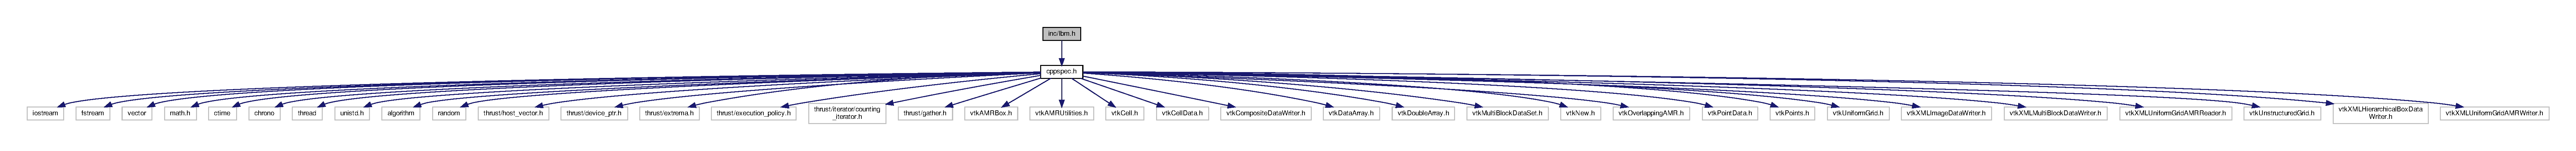
\includegraphics[width=350pt]{lbm_8h__incl}
\end{center}
\end{figure}
This graph shows which files directly or indirectly include this file\+:
\nopagebreak
\begin{figure}[H]
\begin{center}
\leavevmode
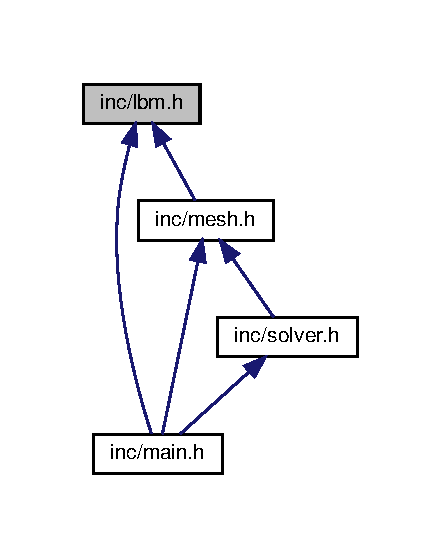
\includegraphics[width=212pt]{lbm_8h__dep__incl}
\end{center}
\end{figure}
\subsection*{Macros}
\begin{DoxyCompactItemize}
\item 
\#define \hyperlink{lbm_8h_acfb5feff3d74c31fd8abe42a30a1f769}{l\+\_\+dq}~27
\begin{DoxyCompactList}\small\item\em Number of particle velocity vectors in the discretized particle velocity set. \end{DoxyCompactList}\item 
\#define \hyperlink{lbm_8h_a7702b5f02aa4d220fad9dea224c4b519}{l\+\_\+dq\+\_\+max}~27
\begin{DoxyCompactList}\small\item\em Number of particle velocity vectors requried for complete connectivity. \end{DoxyCompactList}\item 
\#define \hyperlink{lbm_8h_aba8902900fa07ff44dbb4a739c0e5163}{cs}~0.\+5773503F
\begin{DoxyCompactList}\small\item\em Macro definition for lattice speed of sound (1/sqrt(3)). \end{DoxyCompactList}\item 
\#define \hyperlink{lbm_8h_aee6f45fcdff121ba7a5621ce6181ac86}{cs2}~0.\+3333333F
\begin{DoxyCompactList}\small\item\em Macro definition for \hyperlink{lbm_8h_aba8902900fa07ff44dbb4a739c0e5163}{cs} squared. \end{DoxyCompactList}\item 
\#define \hyperlink{lbm_8h_ae7a226ba3e1299f9c0bdf1cc76e7d5d8}{cs4}~0.\+1111111F
\begin{DoxyCompactList}\small\item\em Macro definition for \hyperlink{lbm_8h_aee6f45fcdff121ba7a5621ce6181ac86}{cs2} squared. \end{DoxyCompactList}\item 
\#define \hyperlink{lbm_8h_ab4bd27eb9c007776af9764a4ee4971d4}{cso2}~3.\+0000000F
\begin{DoxyCompactList}\small\item\em Macro definition for inverse of \hyperlink{lbm_8h_aee6f45fcdff121ba7a5621ce6181ac86}{cs2}. \end{DoxyCompactList}\item 
\#define \hyperlink{lbm_8h_aa684160cf8490a8372628d8178eb0efa}{hcso2}~1.\+5000000F
\begin{DoxyCompactList}\small\item\em Macro definition for half of \hyperlink{lbm_8h_ab4bd27eb9c007776af9764a4ee4971d4}{cso2}. \end{DoxyCompactList}\item 
\#define \hyperlink{lbm_8h_a64b5e00638a22c45514a8fb8a9554209}{hcso4}~4.\+5000000F
\begin{DoxyCompactList}\small\item\em Macro definition for half of inverse of \hyperlink{lbm_8h_ae7a226ba3e1299f9c0bdf1cc76e7d5d8}{cs4}. \end{DoxyCompactList}\end{DoxyCompactItemize}
\subsection*{Variables}
\begin{DoxyCompactItemize}
\item 
const double \hyperlink{lbm_8h_aedababd215e10df9a0429120bba1660a}{w} \mbox{[}2\mbox{]}\mbox{[}27\mbox{]}
\begin{DoxyCompactList}\small\item\em Array of Gauss-\/\+Hermite quadrature weights for corresponding discrete particle velocity set. \end{DoxyCompactList}\item 
const double \hyperlink{lbm_8h_ab572a119792cba4003eee82b59009257}{c} \mbox{[}2\mbox{]}\mbox{[}27 $\ast$3\mbox{]}
\begin{DoxyCompactList}\small\item\em Array of velocity vectors for corresponding discrete particle velocity set. \end{DoxyCompactList}\item 
const int \hyperlink{lbm_8h_a1f1eab5cc6ba79f67155799525885861}{pb} \mbox{[}2\mbox{]}\mbox{[}27\mbox{]}
\begin{DoxyCompactList}\small\item\em Array of indices for reflected velocity vectors for corresponding discrete particle velocity set. \end{DoxyCompactList}\end{DoxyCompactItemize}


\subsection{Macro Definition Documentation}
\mbox{\Hypertarget{lbm_8h_aba8902900fa07ff44dbb4a739c0e5163}\label{lbm_8h_aba8902900fa07ff44dbb4a739c0e5163}} 
\index{lbm.\+h@{lbm.\+h}!cs@{cs}}
\index{cs@{cs}!lbm.\+h@{lbm.\+h}}
\subsubsection{\texorpdfstring{cs}{cs}}
{\footnotesize\ttfamily \#define cs~0.\+5773503F}



Macro definition for lattice speed of sound (1/sqrt(3)). 

\mbox{\Hypertarget{lbm_8h_aee6f45fcdff121ba7a5621ce6181ac86}\label{lbm_8h_aee6f45fcdff121ba7a5621ce6181ac86}} 
\index{lbm.\+h@{lbm.\+h}!cs2@{cs2}}
\index{cs2@{cs2}!lbm.\+h@{lbm.\+h}}
\subsubsection{\texorpdfstring{cs2}{cs2}}
{\footnotesize\ttfamily \#define cs2~0.\+3333333F}



Macro definition for \hyperlink{lbm_8h_aba8902900fa07ff44dbb4a739c0e5163}{cs} squared. 

\mbox{\Hypertarget{lbm_8h_ae7a226ba3e1299f9c0bdf1cc76e7d5d8}\label{lbm_8h_ae7a226ba3e1299f9c0bdf1cc76e7d5d8}} 
\index{lbm.\+h@{lbm.\+h}!cs4@{cs4}}
\index{cs4@{cs4}!lbm.\+h@{lbm.\+h}}
\subsubsection{\texorpdfstring{cs4}{cs4}}
{\footnotesize\ttfamily \#define cs4~0.\+1111111F}



Macro definition for \hyperlink{lbm_8h_aee6f45fcdff121ba7a5621ce6181ac86}{cs2} squared. 

\mbox{\Hypertarget{lbm_8h_ab4bd27eb9c007776af9764a4ee4971d4}\label{lbm_8h_ab4bd27eb9c007776af9764a4ee4971d4}} 
\index{lbm.\+h@{lbm.\+h}!cso2@{cso2}}
\index{cso2@{cso2}!lbm.\+h@{lbm.\+h}}
\subsubsection{\texorpdfstring{cso2}{cso2}}
{\footnotesize\ttfamily \#define cso2~3.\+0000000F}



Macro definition for inverse of \hyperlink{lbm_8h_aee6f45fcdff121ba7a5621ce6181ac86}{cs2}. 

\mbox{\Hypertarget{lbm_8h_aa684160cf8490a8372628d8178eb0efa}\label{lbm_8h_aa684160cf8490a8372628d8178eb0efa}} 
\index{lbm.\+h@{lbm.\+h}!hcso2@{hcso2}}
\index{hcso2@{hcso2}!lbm.\+h@{lbm.\+h}}
\subsubsection{\texorpdfstring{hcso2}{hcso2}}
{\footnotesize\ttfamily \#define hcso2~1.\+5000000F}



Macro definition for half of \hyperlink{lbm_8h_ab4bd27eb9c007776af9764a4ee4971d4}{cso2}. 

\mbox{\Hypertarget{lbm_8h_a64b5e00638a22c45514a8fb8a9554209}\label{lbm_8h_a64b5e00638a22c45514a8fb8a9554209}} 
\index{lbm.\+h@{lbm.\+h}!hcso4@{hcso4}}
\index{hcso4@{hcso4}!lbm.\+h@{lbm.\+h}}
\subsubsection{\texorpdfstring{hcso4}{hcso4}}
{\footnotesize\ttfamily \#define hcso4~4.\+5000000F}



Macro definition for half of inverse of \hyperlink{lbm_8h_ae7a226ba3e1299f9c0bdf1cc76e7d5d8}{cs4}. 

\mbox{\Hypertarget{lbm_8h_acfb5feff3d74c31fd8abe42a30a1f769}\label{lbm_8h_acfb5feff3d74c31fd8abe42a30a1f769}} 
\index{lbm.\+h@{lbm.\+h}!l\+\_\+dq@{l\+\_\+dq}}
\index{l\+\_\+dq@{l\+\_\+dq}!lbm.\+h@{lbm.\+h}}
\subsubsection{\texorpdfstring{l\+\_\+dq}{l\_dq}}
{\footnotesize\ttfamily \#define l\+\_\+dq~27}



Number of particle velocity vectors in the discretized particle velocity set. 

When \hyperlink{cppspec_8h_a327d0faa306d7663502be8df312a815e}{N\+\_\+\+D\+IM} = 2, this is equal to 9 (i.\+e. D2\+Q9). In 3D, this value is set to 19 by default (i.\+e. D3\+Q19) but can be set to 27 for D3\+Q27 as well. \mbox{\Hypertarget{lbm_8h_a7702b5f02aa4d220fad9dea224c4b519}\label{lbm_8h_a7702b5f02aa4d220fad9dea224c4b519}} 
\index{lbm.\+h@{lbm.\+h}!l\+\_\+dq\+\_\+max@{l\+\_\+dq\+\_\+max}}
\index{l\+\_\+dq\+\_\+max@{l\+\_\+dq\+\_\+max}!lbm.\+h@{lbm.\+h}}
\subsubsection{\texorpdfstring{l\+\_\+dq\+\_\+max}{l\_dq\_max}}
{\footnotesize\ttfamily \#define l\+\_\+dq\+\_\+max~27}



Number of particle velocity vectors requried for complete connectivity. 

This value is equal to \hyperlink{lbm_8h_acfb5feff3d74c31fd8abe42a30a1f769}{l\+\_\+dq} in 2D but equal to the D3\+Q27 amount in 3D (whereas \hyperlink{lbm_8h_acfb5feff3d74c31fd8abe42a30a1f769}{l\+\_\+dq} can take on separate values for D3\+Q19 and D3\+Q27). 

\subsection{Variable Documentation}
\mbox{\Hypertarget{lbm_8h_ab572a119792cba4003eee82b59009257}\label{lbm_8h_ab572a119792cba4003eee82b59009257}} 
\index{lbm.\+h@{lbm.\+h}!c@{c}}
\index{c@{c}!lbm.\+h@{lbm.\+h}}
\subsubsection{\texorpdfstring{c}{c}}
{\footnotesize\ttfamily const double c\mbox{[}2\mbox{]}\mbox{[}27 $\ast$3\mbox{]}}

{\bfseries Initial value\+:}
\begin{DoxyCode}
=
\{\{ 0,1,0,-1,0,1,-1,-1,1,   0,0,1,0,-1,1,1,-1,-1\},
\{ 0,1,-1,0,0,0,0,1,-1,1,-1,0,0,1,-1,1,-1,0,0,1,-1,1,-1,1,-1,-1,1,   0,0,0,1,-1,0,0,1,-1,0,0,1,-1,-1,1,0,0,1
      ,-1,1,-1,1,-1,-1,1,1,-1,   0,0,0,0,0,1,-1,0,0,1,-1,1,-1,0,0,-1,1,-1,1,1,-1,-1,1,1,-1,1,-1 \}\}
\end{DoxyCode}


Array of velocity vectors for corresponding discrete particle velocity set. 

\mbox{\Hypertarget{lbm_8h_a1f1eab5cc6ba79f67155799525885861}\label{lbm_8h_a1f1eab5cc6ba79f67155799525885861}} 
\index{lbm.\+h@{lbm.\+h}!pb@{pb}}
\index{pb@{pb}!lbm.\+h@{lbm.\+h}}
\subsubsection{\texorpdfstring{pb}{pb}}
{\footnotesize\ttfamily const int pb\mbox{[}2\mbox{]}\mbox{[}27\mbox{]}}

{\bfseries Initial value\+:}
\begin{DoxyCode}
=
\{\{0,3,4,1,2,7,8,5,6\},
\{0,2,1,4,3,6,5,8,7,10,9,12,11,14,13,16,15,18,17,20,19,22,21,24,23,26,25\}\}
\end{DoxyCode}


Array of indices for reflected velocity vectors for corresponding discrete particle velocity set. 

\mbox{\Hypertarget{lbm_8h_aedababd215e10df9a0429120bba1660a}\label{lbm_8h_aedababd215e10df9a0429120bba1660a}} 
\index{lbm.\+h@{lbm.\+h}!w@{w}}
\index{w@{w}!lbm.\+h@{lbm.\+h}}
\subsubsection{\texorpdfstring{w}{w}}
{\footnotesize\ttfamily const double w\mbox{[}2\mbox{]}\mbox{[}27\mbox{]}}

{\bfseries Initial value\+:}
\begin{DoxyCode}
= 
\{\{4.0/9.0,1.0/9.0,1.0/9.0,1.0/9.0,1.0/9.0,1.0/36.0,1.0/36.0,1.0/36.0,1.0/36.0\},



\{8.0/27.0,2.0/27.0,2.0/27.0,2.0/27.0,2.0/27.0,2.0/27.0,2.0/27.0,1.0/54.0,1.0/54.0,1.0/54.0,1.0/54.0,1.0/54.
      0,1.0/54.0,1.0/54.0,1.0/54.0,1.0/54.0,1.0/54.0,1.0/54.0,1.0/54.0,1.0/216.0,1.0/216.0,1.0/216.0,1.0/216.0,1.0
      /216.0,1.0/216.0,1.0/216.0,1.0/216.0\}\}
\end{DoxyCode}


Array of Gauss-\/\+Hermite quadrature weights for corresponding discrete particle velocity set. 


\hypertarget{main_8h}{}\section{inc/main.h File Reference}
\label{main_8h}\index{inc/main.\+h@{inc/main.\+h}}
{\ttfamily \#include \char`\"{}lbm.\+h\char`\"{}}\newline
{\ttfamily \#include \char`\"{}mesh.\+h\char`\"{}}\newline
{\ttfamily \#include \char`\"{}solver.\+h\char`\"{}}\newline
Include dependency graph for main.\+h\+:
\nopagebreak
\begin{figure}[H]
\begin{center}
\leavevmode
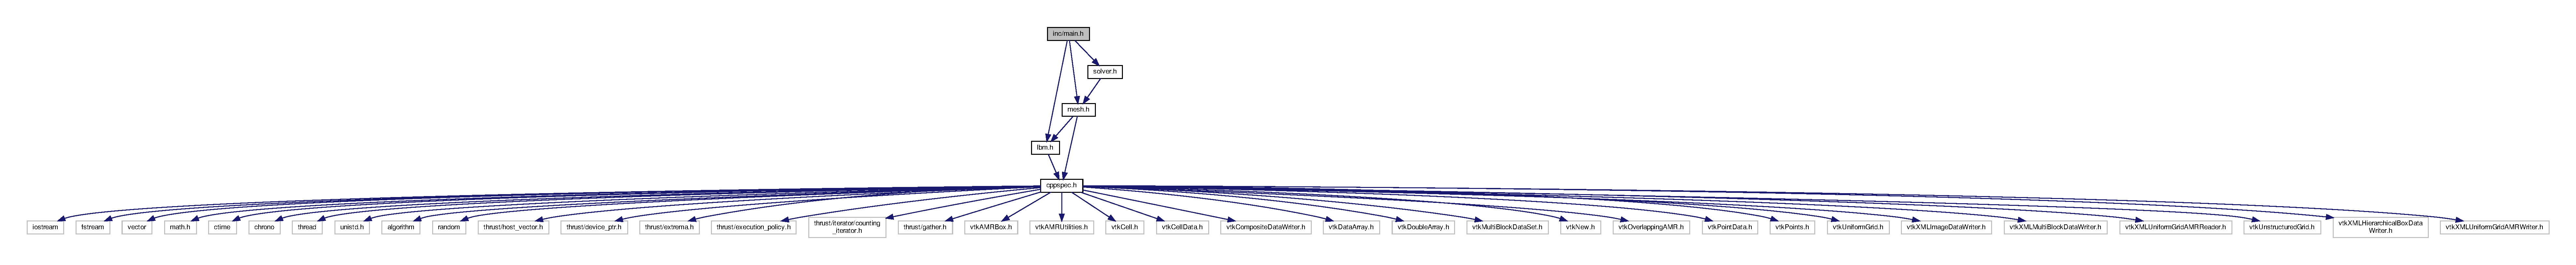
\includegraphics[width=350pt]{main_8h__incl}
\end{center}
\end{figure}

\hypertarget{mesh_8h}{}\section{inc/mesh.h File Reference}
\label{mesh_8h}\index{inc/mesh.\+h@{inc/mesh.\+h}}
{\ttfamily \#include \char`\"{}cppspec.\+h\char`\"{}}\newline
{\ttfamily \#include \char`\"{}lbm.\+h\char`\"{}}\newline
Include dependency graph for mesh.\+h\+:
\nopagebreak
\begin{figure}[H]
\begin{center}
\leavevmode
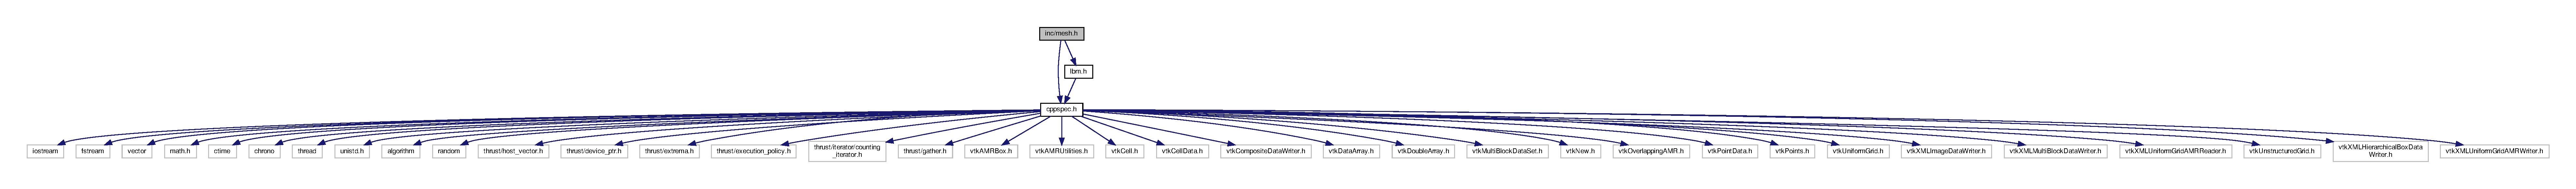
\includegraphics[width=350pt]{mesh_8h__incl}
\end{center}
\end{figure}
This graph shows which files directly or indirectly include this file\+:
\nopagebreak
\begin{figure}[H]
\begin{center}
\leavevmode
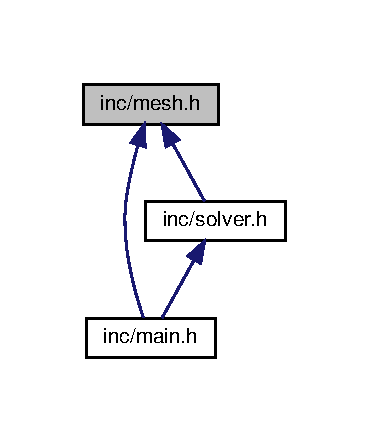
\includegraphics[width=177pt]{mesh_8h__dep__incl}
\end{center}
\end{figure}
\subsection*{Classes}
\begin{DoxyCompactItemize}
\item 
class \hyperlink{classMesh}{Mesh}
\begin{DoxyCompactList}\small\item\em The mesh class. \end{DoxyCompactList}\end{DoxyCompactItemize}
\subsection*{Macros}
\begin{DoxyCompactItemize}
\item 
\#define \hyperlink{mesh_8h_abc6c2c98ea8adb0f4f86cc65376a92c6}{V\+\_\+\+R\+E\+F\+\_\+\+I\+D\+\_\+\+U\+N\+R\+E\+F\+I\+N\+ED}~0
\begin{DoxyCompactList}\small\item\em Indicates cell-\/block is unrefined. \end{DoxyCompactList}\item 
\#define \hyperlink{mesh_8h_ad7eb161e8411b6d1c5323e08f94cbeca}{V\+\_\+\+R\+E\+F\+\_\+\+I\+D\+\_\+\+U\+N\+R\+E\+F\+I\+N\+E\+D\+\_\+\+V\+IO}~9
\begin{DoxyCompactList}\small\item\em Indicates cell-\/block is unrefined by possibly violating a quality-\/control criterion. \end{DoxyCompactList}\item 
\#define \hyperlink{mesh_8h_a9a62df1058077bce4db0d72d9146a28c}{V\+\_\+\+R\+E\+F\+\_\+\+I\+D\+\_\+\+R\+E\+F\+I\+N\+ED}~1
\begin{DoxyCompactList}\small\item\em Indicates cell-\/block is refined. \end{DoxyCompactList}\item 
\#define \hyperlink{mesh_8h_a69ce872b476f502cbe80db24a104fa41}{V\+\_\+\+R\+E\+F\+\_\+\+I\+D\+\_\+\+R\+E\+F\+I\+N\+E\+D\+\_\+\+W\+C\+H\+I\+LD}~2
\begin{DoxyCompactList}\small\item\em Indicates cell-\/block is refined and has at least one refined child. \end{DoxyCompactList}\item 
\#define \hyperlink{mesh_8h_add82df4941e230cb83f4737b31207c3d}{V\+\_\+\+R\+E\+F\+\_\+\+I\+D\+\_\+\+R\+E\+F\+I\+N\+E\+D\+\_\+\+P\+E\+RM}~3
\begin{DoxyCompactList}\small\item\em Indicates cell-\/block is refined permanently (mainly for near-\/wall stability). \end{DoxyCompactList}\item 
\#define \hyperlink{mesh_8h_a302ea61cf675f06725e367907dfc7fb7}{V\+\_\+\+R\+E\+F\+\_\+\+I\+D\+\_\+\+R\+E\+F\+I\+N\+E\+D\+\_\+\+W\+C\+H\+I\+L\+D\+\_\+\+P\+E\+RM}~10
\begin{DoxyCompactList}\small\item\em Indicates cell-\/block is refined permanently (mainly for near-\/wall stability). \end{DoxyCompactList}\item 
\#define \hyperlink{mesh_8h_af2d286018fc7442a20b7525b39829c1f}{V\+\_\+\+R\+E\+F\+\_\+\+I\+D\+\_\+\+M\+A\+R\+K\+\_\+\+R\+E\+F\+I\+NE}~4
\begin{DoxyCompactList}\small\item\em Indicates cell-\/block is marked for refinement. \end{DoxyCompactList}\item 
\#define \hyperlink{mesh_8h_a0656aa177812f4b7aa35121197e60038}{V\+\_\+\+R\+E\+F\+\_\+\+I\+D\+\_\+\+M\+A\+R\+K\+\_\+\+C\+O\+A\+R\+S\+EN}~5
\begin{DoxyCompactList}\small\item\em Indicates cell-\/block is marked for coarsening. \end{DoxyCompactList}\item 
\#define \hyperlink{mesh_8h_a88587c2c945f1135189c3bd59b4f34bd}{V\+\_\+\+R\+E\+F\+\_\+\+I\+D\+\_\+\+N\+EW}~6
\begin{DoxyCompactList}\small\item\em Indicates cell-\/block was newly inserted (as a child). \end{DoxyCompactList}\item 
\#define \hyperlink{mesh_8h_ae403a731f76ee11227a686c5aa3770e0}{V\+\_\+\+R\+E\+F\+\_\+\+I\+D\+\_\+\+R\+E\+M\+O\+VE}~7
\begin{DoxyCompactList}\small\item\em Indicates cell-\/block will be removed (as a child). \end{DoxyCompactList}\item 
\#define \hyperlink{mesh_8h_abec9ea9c0a2893d8ee04a695ed155a95}{V\+\_\+\+R\+E\+F\+\_\+\+I\+D\+\_\+\+I\+N\+A\+C\+T\+I\+VE}~8
\begin{DoxyCompactList}\small\item\em Indicates cell-\/block is inactive in the simulation. \end{DoxyCompactList}\item 
\#define \hyperlink{mesh_8h_a1a188abc73dbd5a4ee12addffb550f2f}{V\+\_\+\+I\+N\+T\+E\+R\+P\+\_\+\+U\+N\+I\+F\+O\+R\+M\+\_\+F}~0
\begin{DoxyCompactList}\small\item\em A. \end{DoxyCompactList}\item 
\#define \hyperlink{mesh_8h_a7f94fa8ca1abcfaec3ed6122459bd478}{V\+\_\+\+I\+N\+T\+E\+RP}~U\+N\+I\+F\+O\+R\+M\+\_\+\+Fs		1
\begin{DoxyCompactList}\small\item\em A. \end{DoxyCompactList}\item 
\#define \hyperlink{mesh_8h_a8ba83547ea695457721123ee457d3332}{V\+\_\+\+I\+N\+T\+E\+R\+P\+\_\+\+C\+U\+B\+I\+C\+\_\+F}~2
\begin{DoxyCompactList}\small\item\em A. \end{DoxyCompactList}\item 
\#define \hyperlink{mesh_8h_a0a98278da8a7ebc85f3bb387ab9a4bfe}{V\+\_\+\+I\+N\+T\+E\+R\+P\+\_\+\+C\+U\+B\+I\+C\+\_\+\+Fs}~3
\begin{DoxyCompactList}\small\item\em A. \end{DoxyCompactList}\item 
\#define \hyperlink{mesh_8h_a78dcc090e2a73c495fc39a8be424c018}{V\+\_\+\+I\+N\+T\+E\+R\+P\+\_\+\+A\+D\+D\+E\+D\+\_\+F}~4
\begin{DoxyCompactList}\small\item\em A. \end{DoxyCompactList}\item 
\#define \hyperlink{mesh_8h_a12461b570df9612c34767dfe93232490}{V\+\_\+\+I\+N\+T\+E\+R\+P\+\_\+\+A\+D\+D\+E\+D\+\_\+\+Fs}~5
\begin{DoxyCompactList}\small\item\em A. \end{DoxyCompactList}\item 
\#define \hyperlink{mesh_8h_ad75741e1a7841d54c98aaf4670e3468a}{V\+\_\+\+A\+V\+E\+R\+A\+G\+E\+\_\+F}~0
\begin{DoxyCompactList}\small\item\em A. \end{DoxyCompactList}\item 
\#define \hyperlink{mesh_8h_a89a126a1107e3ca976cee1fde7af77e4}{V\+\_\+\+A\+D\+V\+\_\+\+T\+Y\+P\+E\+\_\+\+U\+N\+I\+F\+O\+RM}~0
\begin{DoxyCompactList}\small\item\em A. \end{DoxyCompactList}\item 
\#define \hyperlink{mesh_8h_a51c6161c29676b87695bab3438ddd06c}{V\+\_\+\+A\+D\+V\+\_\+\+T\+Y\+P\+E\+\_\+\+C\+U\+B\+IC}~2
\begin{DoxyCompactList}\small\item\em A. \end{DoxyCompactList}\item 
\#define \hyperlink{mesh_8h_a6df941794c7052c2ba063eaab92e48e9}{V\+\_\+\+A\+D\+V\+\_\+\+T\+Y\+PE}~\hyperlink{mesh_8h_a51c6161c29676b87695bab3438ddd06c}{V\+\_\+\+A\+D\+V\+\_\+\+T\+Y\+P\+E\+\_\+\+C\+U\+B\+IC}
\begin{DoxyCompactList}\small\item\em A. \end{DoxyCompactList}\item 
\#define \hyperlink{mesh_8h_a5465378332c79eb52e353600ad3dfe99}{V\+\_\+\+R\+E\+S\+C\+A\+L\+E\+\_\+\+T\+Y\+PE}~0
\item 
\#define \hyperlink{mesh_8h_a5465378332c79eb52e353600ad3dfe99}{V\+\_\+\+R\+E\+S\+C\+A\+L\+E\+\_\+\+T\+Y\+PE}~1
\end{DoxyCompactItemize}
\subsection*{Functions}
\begin{DoxyCompactItemize}
\item 
{\footnotesize template$<$class T $>$ }\\\+\_\+\+\_\+global\+\_\+\+\_\+ void \hyperlink{mesh_8h_a6fa64fed754b5aa2db345680d30c34ba}{Cu\+\_\+\+Reset\+To\+Value} (int N, T $\ast$arr, T val)
\begin{DoxyCompactList}\small\item\em Reset values of G\+PU array. \end{DoxyCompactList}\item 
{\footnotesize template$<$class T $>$ }\\\+\_\+\+\_\+global\+\_\+\+\_\+ void \hyperlink{mesh_8h_afe0417e381d21a938cc312cfad4d816e}{Cu\+\_\+\+Contract\+By\+Frac} (int N, T $\ast$arr, int frac, T $\ast$arr2)
\begin{DoxyCompactList}\small\item\em Contract array elements by a specified amount. \end{DoxyCompactList}\item 
{\footnotesize template$<$class T $>$ }\\\+\_\+\+\_\+global\+\_\+\+\_\+ void \hyperlink{mesh_8h_a478831a86e6d0a1151ee26218d9cf0eb}{Cu\+\_\+\+Fill\+Linear} (int N, T $\ast$arr)
\begin{DoxyCompactList}\small\item\em Fill an array with a value equal to the index. \end{DoxyCompactList}\end{DoxyCompactItemize}
\subsection*{Variables}
\begin{DoxyCompactItemize}
\item 
const int \hyperlink{mesh_8h_a10f21bd2ce1bac58c942c5bb17c1b026}{str2aschild} \mbox{[}2\mbox{]}\mbox{[}8\mbox{]}
\item 
const double \hyperlink{mesh_8h_a2cd23a9c4c130f6ceec68bc7a97dba6c}{dx\+\_\+vec} \mbox{[}2\mbox{]}\mbox{[}3 $\ast$8\mbox{]}
\item 
const int \hyperlink{mesh_8h_a7ee37d8276f9af262711df33fea3f6cc}{child\+\_\+id\+\_\+switch} \mbox{[}\hyperlink{cppspec_8h_a39646502414a17a8518d029263259eee}{N\+\_\+\+C\+H\+I\+L\+D\+R\+EN}\mbox{]}
\item 
int \hyperlink{mesh_8h_a5f5bf4c2b26e229a3053120991eff3bf}{child\+\_\+nbrs} \mbox{[}2\mbox{]}\mbox{[}8 $\ast$27\mbox{]}
\item 
int \hyperlink{mesh_8h_aca31b22b369316a7b07d015b30c59239}{child\+\_\+nbrs\+\_\+I} \mbox{[}2\mbox{]}\mbox{[}8 $\ast$27\mbox{]}
\item 
int \hyperlink{mesh_8h_aebda8a2ee3ebd37db947206b7cf982d6}{advancement\+\_\+ids} \mbox{[}2\mbox{]}\mbox{[}27 $\ast$27\mbox{]}
\item 
int \hyperlink{mesh_8h_a9056ba1955d628cdc00230d6ab5c80d3}{interp\+\_\+ids} \mbox{[}2\mbox{]}\mbox{[}8 $\ast$8\mbox{]}
\item 
\hyperlink{cppspec_8h_af529d360dfac9b9578aa719418a53a21}{ufloat\+\_\+t} \hyperlink{mesh_8h_ae94f0f7281620ce67c60ae012cd52ee8}{interp\+\_\+coeffs} \mbox{[}2\mbox{]}\mbox{[}(8 $\ast$8) $\ast$8\mbox{]}
\item 
const double \hyperlink{mesh_8h_a55c0e97fcc9a3a4896115c0b088cc5f0}{init\+\_\+grid\+\_\+x} \mbox{[}\hyperlink{cppspec_8h_ab6471b0dc18a88669e137a1223f9cad8}{Nx2}\mbox{]}
\item 
const double \hyperlink{mesh_8h_a7c4c84405f89d81bb9c14771db38bf04}{init\+\_\+grid\+\_\+y} \mbox{[}\hyperlink{cppspec_8h_ab6471b0dc18a88669e137a1223f9cad8}{Nx2}\mbox{]}
\end{DoxyCompactItemize}


\subsection{Macro Definition Documentation}
\mbox{\Hypertarget{mesh_8h_a6df941794c7052c2ba063eaab92e48e9}\label{mesh_8h_a6df941794c7052c2ba063eaab92e48e9}} 
\index{mesh.\+h@{mesh.\+h}!V\+\_\+\+A\+D\+V\+\_\+\+T\+Y\+PE@{V\+\_\+\+A\+D\+V\+\_\+\+T\+Y\+PE}}
\index{V\+\_\+\+A\+D\+V\+\_\+\+T\+Y\+PE@{V\+\_\+\+A\+D\+V\+\_\+\+T\+Y\+PE}!mesh.\+h@{mesh.\+h}}
\subsubsection{\texorpdfstring{V\+\_\+\+A\+D\+V\+\_\+\+T\+Y\+PE}{V\_ADV\_TYPE}}
{\footnotesize\ttfamily \#define V\+\_\+\+A\+D\+V\+\_\+\+T\+Y\+PE~\hyperlink{mesh_8h_a51c6161c29676b87695bab3438ddd06c}{V\+\_\+\+A\+D\+V\+\_\+\+T\+Y\+P\+E\+\_\+\+C\+U\+B\+IC}}



A. 

\mbox{\Hypertarget{mesh_8h_a51c6161c29676b87695bab3438ddd06c}\label{mesh_8h_a51c6161c29676b87695bab3438ddd06c}} 
\index{mesh.\+h@{mesh.\+h}!V\+\_\+\+A\+D\+V\+\_\+\+T\+Y\+P\+E\+\_\+\+C\+U\+B\+IC@{V\+\_\+\+A\+D\+V\+\_\+\+T\+Y\+P\+E\+\_\+\+C\+U\+B\+IC}}
\index{V\+\_\+\+A\+D\+V\+\_\+\+T\+Y\+P\+E\+\_\+\+C\+U\+B\+IC@{V\+\_\+\+A\+D\+V\+\_\+\+T\+Y\+P\+E\+\_\+\+C\+U\+B\+IC}!mesh.\+h@{mesh.\+h}}
\subsubsection{\texorpdfstring{V\+\_\+\+A\+D\+V\+\_\+\+T\+Y\+P\+E\+\_\+\+C\+U\+B\+IC}{V\_ADV\_TYPE\_CUBIC}}
{\footnotesize\ttfamily \#define V\+\_\+\+A\+D\+V\+\_\+\+T\+Y\+P\+E\+\_\+\+C\+U\+B\+IC~2}



A. 

\mbox{\Hypertarget{mesh_8h_a89a126a1107e3ca976cee1fde7af77e4}\label{mesh_8h_a89a126a1107e3ca976cee1fde7af77e4}} 
\index{mesh.\+h@{mesh.\+h}!V\+\_\+\+A\+D\+V\+\_\+\+T\+Y\+P\+E\+\_\+\+U\+N\+I\+F\+O\+RM@{V\+\_\+\+A\+D\+V\+\_\+\+T\+Y\+P\+E\+\_\+\+U\+N\+I\+F\+O\+RM}}
\index{V\+\_\+\+A\+D\+V\+\_\+\+T\+Y\+P\+E\+\_\+\+U\+N\+I\+F\+O\+RM@{V\+\_\+\+A\+D\+V\+\_\+\+T\+Y\+P\+E\+\_\+\+U\+N\+I\+F\+O\+RM}!mesh.\+h@{mesh.\+h}}
\subsubsection{\texorpdfstring{V\+\_\+\+A\+D\+V\+\_\+\+T\+Y\+P\+E\+\_\+\+U\+N\+I\+F\+O\+RM}{V\_ADV\_TYPE\_UNIFORM}}
{\footnotesize\ttfamily \#define V\+\_\+\+A\+D\+V\+\_\+\+T\+Y\+P\+E\+\_\+\+U\+N\+I\+F\+O\+RM~0}



A. 

\mbox{\Hypertarget{mesh_8h_ad75741e1a7841d54c98aaf4670e3468a}\label{mesh_8h_ad75741e1a7841d54c98aaf4670e3468a}} 
\index{mesh.\+h@{mesh.\+h}!V\+\_\+\+A\+V\+E\+R\+A\+G\+E\+\_\+F@{V\+\_\+\+A\+V\+E\+R\+A\+G\+E\+\_\+F}}
\index{V\+\_\+\+A\+V\+E\+R\+A\+G\+E\+\_\+F@{V\+\_\+\+A\+V\+E\+R\+A\+G\+E\+\_\+F}!mesh.\+h@{mesh.\+h}}
\subsubsection{\texorpdfstring{V\+\_\+\+A\+V\+E\+R\+A\+G\+E\+\_\+F}{V\_AVERAGE\_F}}
{\footnotesize\ttfamily \#define V\+\_\+\+A\+V\+E\+R\+A\+G\+E\+\_\+F~0}



A. 

\mbox{\Hypertarget{mesh_8h_a7f94fa8ca1abcfaec3ed6122459bd478}\label{mesh_8h_a7f94fa8ca1abcfaec3ed6122459bd478}} 
\index{mesh.\+h@{mesh.\+h}!V\+\_\+\+I\+N\+T\+E\+RP@{V\+\_\+\+I\+N\+T\+E\+RP}}
\index{V\+\_\+\+I\+N\+T\+E\+RP@{V\+\_\+\+I\+N\+T\+E\+RP}!mesh.\+h@{mesh.\+h}}
\subsubsection{\texorpdfstring{V\+\_\+\+I\+N\+T\+E\+RP}{V\_INTERP}}
{\footnotesize\ttfamily \#define V\+\_\+\+I\+N\+T\+E\+RP~U\+N\+I\+F\+O\+R\+M\+\_\+\+Fs		1}



A. 

\mbox{\Hypertarget{mesh_8h_a78dcc090e2a73c495fc39a8be424c018}\label{mesh_8h_a78dcc090e2a73c495fc39a8be424c018}} 
\index{mesh.\+h@{mesh.\+h}!V\+\_\+\+I\+N\+T\+E\+R\+P\+\_\+\+A\+D\+D\+E\+D\+\_\+F@{V\+\_\+\+I\+N\+T\+E\+R\+P\+\_\+\+A\+D\+D\+E\+D\+\_\+F}}
\index{V\+\_\+\+I\+N\+T\+E\+R\+P\+\_\+\+A\+D\+D\+E\+D\+\_\+F@{V\+\_\+\+I\+N\+T\+E\+R\+P\+\_\+\+A\+D\+D\+E\+D\+\_\+F}!mesh.\+h@{mesh.\+h}}
\subsubsection{\texorpdfstring{V\+\_\+\+I\+N\+T\+E\+R\+P\+\_\+\+A\+D\+D\+E\+D\+\_\+F}{V\_INTERP\_ADDED\_F}}
{\footnotesize\ttfamily \#define V\+\_\+\+I\+N\+T\+E\+R\+P\+\_\+\+A\+D\+D\+E\+D\+\_\+F~4}



A. 

\mbox{\Hypertarget{mesh_8h_a12461b570df9612c34767dfe93232490}\label{mesh_8h_a12461b570df9612c34767dfe93232490}} 
\index{mesh.\+h@{mesh.\+h}!V\+\_\+\+I\+N\+T\+E\+R\+P\+\_\+\+A\+D\+D\+E\+D\+\_\+\+Fs@{V\+\_\+\+I\+N\+T\+E\+R\+P\+\_\+\+A\+D\+D\+E\+D\+\_\+\+Fs}}
\index{V\+\_\+\+I\+N\+T\+E\+R\+P\+\_\+\+A\+D\+D\+E\+D\+\_\+\+Fs@{V\+\_\+\+I\+N\+T\+E\+R\+P\+\_\+\+A\+D\+D\+E\+D\+\_\+\+Fs}!mesh.\+h@{mesh.\+h}}
\subsubsection{\texorpdfstring{V\+\_\+\+I\+N\+T\+E\+R\+P\+\_\+\+A\+D\+D\+E\+D\+\_\+\+Fs}{V\_INTERP\_ADDED\_Fs}}
{\footnotesize\ttfamily \#define V\+\_\+\+I\+N\+T\+E\+R\+P\+\_\+\+A\+D\+D\+E\+D\+\_\+\+Fs~5}



A. 

\mbox{\Hypertarget{mesh_8h_a8ba83547ea695457721123ee457d3332}\label{mesh_8h_a8ba83547ea695457721123ee457d3332}} 
\index{mesh.\+h@{mesh.\+h}!V\+\_\+\+I\+N\+T\+E\+R\+P\+\_\+\+C\+U\+B\+I\+C\+\_\+F@{V\+\_\+\+I\+N\+T\+E\+R\+P\+\_\+\+C\+U\+B\+I\+C\+\_\+F}}
\index{V\+\_\+\+I\+N\+T\+E\+R\+P\+\_\+\+C\+U\+B\+I\+C\+\_\+F@{V\+\_\+\+I\+N\+T\+E\+R\+P\+\_\+\+C\+U\+B\+I\+C\+\_\+F}!mesh.\+h@{mesh.\+h}}
\subsubsection{\texorpdfstring{V\+\_\+\+I\+N\+T\+E\+R\+P\+\_\+\+C\+U\+B\+I\+C\+\_\+F}{V\_INTERP\_CUBIC\_F}}
{\footnotesize\ttfamily \#define V\+\_\+\+I\+N\+T\+E\+R\+P\+\_\+\+C\+U\+B\+I\+C\+\_\+F~2}



A. 

\mbox{\Hypertarget{mesh_8h_a0a98278da8a7ebc85f3bb387ab9a4bfe}\label{mesh_8h_a0a98278da8a7ebc85f3bb387ab9a4bfe}} 
\index{mesh.\+h@{mesh.\+h}!V\+\_\+\+I\+N\+T\+E\+R\+P\+\_\+\+C\+U\+B\+I\+C\+\_\+\+Fs@{V\+\_\+\+I\+N\+T\+E\+R\+P\+\_\+\+C\+U\+B\+I\+C\+\_\+\+Fs}}
\index{V\+\_\+\+I\+N\+T\+E\+R\+P\+\_\+\+C\+U\+B\+I\+C\+\_\+\+Fs@{V\+\_\+\+I\+N\+T\+E\+R\+P\+\_\+\+C\+U\+B\+I\+C\+\_\+\+Fs}!mesh.\+h@{mesh.\+h}}
\subsubsection{\texorpdfstring{V\+\_\+\+I\+N\+T\+E\+R\+P\+\_\+\+C\+U\+B\+I\+C\+\_\+\+Fs}{V\_INTERP\_CUBIC\_Fs}}
{\footnotesize\ttfamily \#define V\+\_\+\+I\+N\+T\+E\+R\+P\+\_\+\+C\+U\+B\+I\+C\+\_\+\+Fs~3}



A. 

\mbox{\Hypertarget{mesh_8h_a1a188abc73dbd5a4ee12addffb550f2f}\label{mesh_8h_a1a188abc73dbd5a4ee12addffb550f2f}} 
\index{mesh.\+h@{mesh.\+h}!V\+\_\+\+I\+N\+T\+E\+R\+P\+\_\+\+U\+N\+I\+F\+O\+R\+M\+\_\+F@{V\+\_\+\+I\+N\+T\+E\+R\+P\+\_\+\+U\+N\+I\+F\+O\+R\+M\+\_\+F}}
\index{V\+\_\+\+I\+N\+T\+E\+R\+P\+\_\+\+U\+N\+I\+F\+O\+R\+M\+\_\+F@{V\+\_\+\+I\+N\+T\+E\+R\+P\+\_\+\+U\+N\+I\+F\+O\+R\+M\+\_\+F}!mesh.\+h@{mesh.\+h}}
\subsubsection{\texorpdfstring{V\+\_\+\+I\+N\+T\+E\+R\+P\+\_\+\+U\+N\+I\+F\+O\+R\+M\+\_\+F}{V\_INTERP\_UNIFORM\_F}}
{\footnotesize\ttfamily \#define V\+\_\+\+I\+N\+T\+E\+R\+P\+\_\+\+U\+N\+I\+F\+O\+R\+M\+\_\+F~0}



A. 

\mbox{\Hypertarget{mesh_8h_abec9ea9c0a2893d8ee04a695ed155a95}\label{mesh_8h_abec9ea9c0a2893d8ee04a695ed155a95}} 
\index{mesh.\+h@{mesh.\+h}!V\+\_\+\+R\+E\+F\+\_\+\+I\+D\+\_\+\+I\+N\+A\+C\+T\+I\+VE@{V\+\_\+\+R\+E\+F\+\_\+\+I\+D\+\_\+\+I\+N\+A\+C\+T\+I\+VE}}
\index{V\+\_\+\+R\+E\+F\+\_\+\+I\+D\+\_\+\+I\+N\+A\+C\+T\+I\+VE@{V\+\_\+\+R\+E\+F\+\_\+\+I\+D\+\_\+\+I\+N\+A\+C\+T\+I\+VE}!mesh.\+h@{mesh.\+h}}
\subsubsection{\texorpdfstring{V\+\_\+\+R\+E\+F\+\_\+\+I\+D\+\_\+\+I\+N\+A\+C\+T\+I\+VE}{V\_REF\_ID\_INACTIVE}}
{\footnotesize\ttfamily \#define V\+\_\+\+R\+E\+F\+\_\+\+I\+D\+\_\+\+I\+N\+A\+C\+T\+I\+VE~8}



Indicates cell-\/block is inactive in the simulation. 

\mbox{\Hypertarget{mesh_8h_a0656aa177812f4b7aa35121197e60038}\label{mesh_8h_a0656aa177812f4b7aa35121197e60038}} 
\index{mesh.\+h@{mesh.\+h}!V\+\_\+\+R\+E\+F\+\_\+\+I\+D\+\_\+\+M\+A\+R\+K\+\_\+\+C\+O\+A\+R\+S\+EN@{V\+\_\+\+R\+E\+F\+\_\+\+I\+D\+\_\+\+M\+A\+R\+K\+\_\+\+C\+O\+A\+R\+S\+EN}}
\index{V\+\_\+\+R\+E\+F\+\_\+\+I\+D\+\_\+\+M\+A\+R\+K\+\_\+\+C\+O\+A\+R\+S\+EN@{V\+\_\+\+R\+E\+F\+\_\+\+I\+D\+\_\+\+M\+A\+R\+K\+\_\+\+C\+O\+A\+R\+S\+EN}!mesh.\+h@{mesh.\+h}}
\subsubsection{\texorpdfstring{V\+\_\+\+R\+E\+F\+\_\+\+I\+D\+\_\+\+M\+A\+R\+K\+\_\+\+C\+O\+A\+R\+S\+EN}{V\_REF\_ID\_MARK\_COARSEN}}
{\footnotesize\ttfamily \#define V\+\_\+\+R\+E\+F\+\_\+\+I\+D\+\_\+\+M\+A\+R\+K\+\_\+\+C\+O\+A\+R\+S\+EN~5}



Indicates cell-\/block is marked for coarsening. 

\mbox{\Hypertarget{mesh_8h_af2d286018fc7442a20b7525b39829c1f}\label{mesh_8h_af2d286018fc7442a20b7525b39829c1f}} 
\index{mesh.\+h@{mesh.\+h}!V\+\_\+\+R\+E\+F\+\_\+\+I\+D\+\_\+\+M\+A\+R\+K\+\_\+\+R\+E\+F\+I\+NE@{V\+\_\+\+R\+E\+F\+\_\+\+I\+D\+\_\+\+M\+A\+R\+K\+\_\+\+R\+E\+F\+I\+NE}}
\index{V\+\_\+\+R\+E\+F\+\_\+\+I\+D\+\_\+\+M\+A\+R\+K\+\_\+\+R\+E\+F\+I\+NE@{V\+\_\+\+R\+E\+F\+\_\+\+I\+D\+\_\+\+M\+A\+R\+K\+\_\+\+R\+E\+F\+I\+NE}!mesh.\+h@{mesh.\+h}}
\subsubsection{\texorpdfstring{V\+\_\+\+R\+E\+F\+\_\+\+I\+D\+\_\+\+M\+A\+R\+K\+\_\+\+R\+E\+F\+I\+NE}{V\_REF\_ID\_MARK\_REFINE}}
{\footnotesize\ttfamily \#define V\+\_\+\+R\+E\+F\+\_\+\+I\+D\+\_\+\+M\+A\+R\+K\+\_\+\+R\+E\+F\+I\+NE~4}



Indicates cell-\/block is marked for refinement. 

\mbox{\Hypertarget{mesh_8h_a88587c2c945f1135189c3bd59b4f34bd}\label{mesh_8h_a88587c2c945f1135189c3bd59b4f34bd}} 
\index{mesh.\+h@{mesh.\+h}!V\+\_\+\+R\+E\+F\+\_\+\+I\+D\+\_\+\+N\+EW@{V\+\_\+\+R\+E\+F\+\_\+\+I\+D\+\_\+\+N\+EW}}
\index{V\+\_\+\+R\+E\+F\+\_\+\+I\+D\+\_\+\+N\+EW@{V\+\_\+\+R\+E\+F\+\_\+\+I\+D\+\_\+\+N\+EW}!mesh.\+h@{mesh.\+h}}
\subsubsection{\texorpdfstring{V\+\_\+\+R\+E\+F\+\_\+\+I\+D\+\_\+\+N\+EW}{V\_REF\_ID\_NEW}}
{\footnotesize\ttfamily \#define V\+\_\+\+R\+E\+F\+\_\+\+I\+D\+\_\+\+N\+EW~6}



Indicates cell-\/block was newly inserted (as a child). 

\mbox{\Hypertarget{mesh_8h_a9a62df1058077bce4db0d72d9146a28c}\label{mesh_8h_a9a62df1058077bce4db0d72d9146a28c}} 
\index{mesh.\+h@{mesh.\+h}!V\+\_\+\+R\+E\+F\+\_\+\+I\+D\+\_\+\+R\+E\+F\+I\+N\+ED@{V\+\_\+\+R\+E\+F\+\_\+\+I\+D\+\_\+\+R\+E\+F\+I\+N\+ED}}
\index{V\+\_\+\+R\+E\+F\+\_\+\+I\+D\+\_\+\+R\+E\+F\+I\+N\+ED@{V\+\_\+\+R\+E\+F\+\_\+\+I\+D\+\_\+\+R\+E\+F\+I\+N\+ED}!mesh.\+h@{mesh.\+h}}
\subsubsection{\texorpdfstring{V\+\_\+\+R\+E\+F\+\_\+\+I\+D\+\_\+\+R\+E\+F\+I\+N\+ED}{V\_REF\_ID\_REFINED}}
{\footnotesize\ttfamily \#define V\+\_\+\+R\+E\+F\+\_\+\+I\+D\+\_\+\+R\+E\+F\+I\+N\+ED~1}



Indicates cell-\/block is refined. 

\mbox{\Hypertarget{mesh_8h_add82df4941e230cb83f4737b31207c3d}\label{mesh_8h_add82df4941e230cb83f4737b31207c3d}} 
\index{mesh.\+h@{mesh.\+h}!V\+\_\+\+R\+E\+F\+\_\+\+I\+D\+\_\+\+R\+E\+F\+I\+N\+E\+D\+\_\+\+P\+E\+RM@{V\+\_\+\+R\+E\+F\+\_\+\+I\+D\+\_\+\+R\+E\+F\+I\+N\+E\+D\+\_\+\+P\+E\+RM}}
\index{V\+\_\+\+R\+E\+F\+\_\+\+I\+D\+\_\+\+R\+E\+F\+I\+N\+E\+D\+\_\+\+P\+E\+RM@{V\+\_\+\+R\+E\+F\+\_\+\+I\+D\+\_\+\+R\+E\+F\+I\+N\+E\+D\+\_\+\+P\+E\+RM}!mesh.\+h@{mesh.\+h}}
\subsubsection{\texorpdfstring{V\+\_\+\+R\+E\+F\+\_\+\+I\+D\+\_\+\+R\+E\+F\+I\+N\+E\+D\+\_\+\+P\+E\+RM}{V\_REF\_ID\_REFINED\_PERM}}
{\footnotesize\ttfamily \#define V\+\_\+\+R\+E\+F\+\_\+\+I\+D\+\_\+\+R\+E\+F\+I\+N\+E\+D\+\_\+\+P\+E\+RM~3}



Indicates cell-\/block is refined permanently (mainly for near-\/wall stability). 

\mbox{\Hypertarget{mesh_8h_a69ce872b476f502cbe80db24a104fa41}\label{mesh_8h_a69ce872b476f502cbe80db24a104fa41}} 
\index{mesh.\+h@{mesh.\+h}!V\+\_\+\+R\+E\+F\+\_\+\+I\+D\+\_\+\+R\+E\+F\+I\+N\+E\+D\+\_\+\+W\+C\+H\+I\+LD@{V\+\_\+\+R\+E\+F\+\_\+\+I\+D\+\_\+\+R\+E\+F\+I\+N\+E\+D\+\_\+\+W\+C\+H\+I\+LD}}
\index{V\+\_\+\+R\+E\+F\+\_\+\+I\+D\+\_\+\+R\+E\+F\+I\+N\+E\+D\+\_\+\+W\+C\+H\+I\+LD@{V\+\_\+\+R\+E\+F\+\_\+\+I\+D\+\_\+\+R\+E\+F\+I\+N\+E\+D\+\_\+\+W\+C\+H\+I\+LD}!mesh.\+h@{mesh.\+h}}
\subsubsection{\texorpdfstring{V\+\_\+\+R\+E\+F\+\_\+\+I\+D\+\_\+\+R\+E\+F\+I\+N\+E\+D\+\_\+\+W\+C\+H\+I\+LD}{V\_REF\_ID\_REFINED\_WCHILD}}
{\footnotesize\ttfamily \#define V\+\_\+\+R\+E\+F\+\_\+\+I\+D\+\_\+\+R\+E\+F\+I\+N\+E\+D\+\_\+\+W\+C\+H\+I\+LD~2}



Indicates cell-\/block is refined and has at least one refined child. 

\mbox{\Hypertarget{mesh_8h_a302ea61cf675f06725e367907dfc7fb7}\label{mesh_8h_a302ea61cf675f06725e367907dfc7fb7}} 
\index{mesh.\+h@{mesh.\+h}!V\+\_\+\+R\+E\+F\+\_\+\+I\+D\+\_\+\+R\+E\+F\+I\+N\+E\+D\+\_\+\+W\+C\+H\+I\+L\+D\+\_\+\+P\+E\+RM@{V\+\_\+\+R\+E\+F\+\_\+\+I\+D\+\_\+\+R\+E\+F\+I\+N\+E\+D\+\_\+\+W\+C\+H\+I\+L\+D\+\_\+\+P\+E\+RM}}
\index{V\+\_\+\+R\+E\+F\+\_\+\+I\+D\+\_\+\+R\+E\+F\+I\+N\+E\+D\+\_\+\+W\+C\+H\+I\+L\+D\+\_\+\+P\+E\+RM@{V\+\_\+\+R\+E\+F\+\_\+\+I\+D\+\_\+\+R\+E\+F\+I\+N\+E\+D\+\_\+\+W\+C\+H\+I\+L\+D\+\_\+\+P\+E\+RM}!mesh.\+h@{mesh.\+h}}
\subsubsection{\texorpdfstring{V\+\_\+\+R\+E\+F\+\_\+\+I\+D\+\_\+\+R\+E\+F\+I\+N\+E\+D\+\_\+\+W\+C\+H\+I\+L\+D\+\_\+\+P\+E\+RM}{V\_REF\_ID\_REFINED\_WCHILD\_PERM}}
{\footnotesize\ttfamily \#define V\+\_\+\+R\+E\+F\+\_\+\+I\+D\+\_\+\+R\+E\+F\+I\+N\+E\+D\+\_\+\+W\+C\+H\+I\+L\+D\+\_\+\+P\+E\+RM~10}



Indicates cell-\/block is refined permanently (mainly for near-\/wall stability). 

\mbox{\Hypertarget{mesh_8h_ae403a731f76ee11227a686c5aa3770e0}\label{mesh_8h_ae403a731f76ee11227a686c5aa3770e0}} 
\index{mesh.\+h@{mesh.\+h}!V\+\_\+\+R\+E\+F\+\_\+\+I\+D\+\_\+\+R\+E\+M\+O\+VE@{V\+\_\+\+R\+E\+F\+\_\+\+I\+D\+\_\+\+R\+E\+M\+O\+VE}}
\index{V\+\_\+\+R\+E\+F\+\_\+\+I\+D\+\_\+\+R\+E\+M\+O\+VE@{V\+\_\+\+R\+E\+F\+\_\+\+I\+D\+\_\+\+R\+E\+M\+O\+VE}!mesh.\+h@{mesh.\+h}}
\subsubsection{\texorpdfstring{V\+\_\+\+R\+E\+F\+\_\+\+I\+D\+\_\+\+R\+E\+M\+O\+VE}{V\_REF\_ID\_REMOVE}}
{\footnotesize\ttfamily \#define V\+\_\+\+R\+E\+F\+\_\+\+I\+D\+\_\+\+R\+E\+M\+O\+VE~7}



Indicates cell-\/block will be removed (as a child). 

\mbox{\Hypertarget{mesh_8h_abc6c2c98ea8adb0f4f86cc65376a92c6}\label{mesh_8h_abc6c2c98ea8adb0f4f86cc65376a92c6}} 
\index{mesh.\+h@{mesh.\+h}!V\+\_\+\+R\+E\+F\+\_\+\+I\+D\+\_\+\+U\+N\+R\+E\+F\+I\+N\+ED@{V\+\_\+\+R\+E\+F\+\_\+\+I\+D\+\_\+\+U\+N\+R\+E\+F\+I\+N\+ED}}
\index{V\+\_\+\+R\+E\+F\+\_\+\+I\+D\+\_\+\+U\+N\+R\+E\+F\+I\+N\+ED@{V\+\_\+\+R\+E\+F\+\_\+\+I\+D\+\_\+\+U\+N\+R\+E\+F\+I\+N\+ED}!mesh.\+h@{mesh.\+h}}
\subsubsection{\texorpdfstring{V\+\_\+\+R\+E\+F\+\_\+\+I\+D\+\_\+\+U\+N\+R\+E\+F\+I\+N\+ED}{V\_REF\_ID\_UNREFINED}}
{\footnotesize\ttfamily \#define V\+\_\+\+R\+E\+F\+\_\+\+I\+D\+\_\+\+U\+N\+R\+E\+F\+I\+N\+ED~0}



Indicates cell-\/block is unrefined. 

\mbox{\Hypertarget{mesh_8h_ad7eb161e8411b6d1c5323e08f94cbeca}\label{mesh_8h_ad7eb161e8411b6d1c5323e08f94cbeca}} 
\index{mesh.\+h@{mesh.\+h}!V\+\_\+\+R\+E\+F\+\_\+\+I\+D\+\_\+\+U\+N\+R\+E\+F\+I\+N\+E\+D\+\_\+\+V\+IO@{V\+\_\+\+R\+E\+F\+\_\+\+I\+D\+\_\+\+U\+N\+R\+E\+F\+I\+N\+E\+D\+\_\+\+V\+IO}}
\index{V\+\_\+\+R\+E\+F\+\_\+\+I\+D\+\_\+\+U\+N\+R\+E\+F\+I\+N\+E\+D\+\_\+\+V\+IO@{V\+\_\+\+R\+E\+F\+\_\+\+I\+D\+\_\+\+U\+N\+R\+E\+F\+I\+N\+E\+D\+\_\+\+V\+IO}!mesh.\+h@{mesh.\+h}}
\subsubsection{\texorpdfstring{V\+\_\+\+R\+E\+F\+\_\+\+I\+D\+\_\+\+U\+N\+R\+E\+F\+I\+N\+E\+D\+\_\+\+V\+IO}{V\_REF\_ID\_UNREFINED\_VIO}}
{\footnotesize\ttfamily \#define V\+\_\+\+R\+E\+F\+\_\+\+I\+D\+\_\+\+U\+N\+R\+E\+F\+I\+N\+E\+D\+\_\+\+V\+IO~9}



Indicates cell-\/block is unrefined by possibly violating a quality-\/control criterion. 

\mbox{\Hypertarget{mesh_8h_a5465378332c79eb52e353600ad3dfe99}\label{mesh_8h_a5465378332c79eb52e353600ad3dfe99}} 
\index{mesh.\+h@{mesh.\+h}!V\+\_\+\+R\+E\+S\+C\+A\+L\+E\+\_\+\+T\+Y\+PE@{V\+\_\+\+R\+E\+S\+C\+A\+L\+E\+\_\+\+T\+Y\+PE}}
\index{V\+\_\+\+R\+E\+S\+C\+A\+L\+E\+\_\+\+T\+Y\+PE@{V\+\_\+\+R\+E\+S\+C\+A\+L\+E\+\_\+\+T\+Y\+PE}!mesh.\+h@{mesh.\+h}}
\subsubsection{\texorpdfstring{V\+\_\+\+R\+E\+S\+C\+A\+L\+E\+\_\+\+T\+Y\+PE}{V\_RESCALE\_TYPE}\hspace{0.1cm}{\footnotesize\ttfamily [1/2]}}
{\footnotesize\ttfamily \#define V\+\_\+\+R\+E\+S\+C\+A\+L\+E\+\_\+\+T\+Y\+PE~0}

\mbox{\Hypertarget{mesh_8h_a5465378332c79eb52e353600ad3dfe99}\label{mesh_8h_a5465378332c79eb52e353600ad3dfe99}} 
\index{mesh.\+h@{mesh.\+h}!V\+\_\+\+R\+E\+S\+C\+A\+L\+E\+\_\+\+T\+Y\+PE@{V\+\_\+\+R\+E\+S\+C\+A\+L\+E\+\_\+\+T\+Y\+PE}}
\index{V\+\_\+\+R\+E\+S\+C\+A\+L\+E\+\_\+\+T\+Y\+PE@{V\+\_\+\+R\+E\+S\+C\+A\+L\+E\+\_\+\+T\+Y\+PE}!mesh.\+h@{mesh.\+h}}
\subsubsection{\texorpdfstring{V\+\_\+\+R\+E\+S\+C\+A\+L\+E\+\_\+\+T\+Y\+PE}{V\_RESCALE\_TYPE}\hspace{0.1cm}{\footnotesize\ttfamily [2/2]}}
{\footnotesize\ttfamily \#define V\+\_\+\+R\+E\+S\+C\+A\+L\+E\+\_\+\+T\+Y\+PE~1}



\subsection{Function Documentation}
\mbox{\Hypertarget{mesh_8h_afe0417e381d21a938cc312cfad4d816e}\label{mesh_8h_afe0417e381d21a938cc312cfad4d816e}} 
\index{mesh.\+h@{mesh.\+h}!Cu\+\_\+\+Contract\+By\+Frac@{Cu\+\_\+\+Contract\+By\+Frac}}
\index{Cu\+\_\+\+Contract\+By\+Frac@{Cu\+\_\+\+Contract\+By\+Frac}!mesh.\+h@{mesh.\+h}}
\subsubsection{\texorpdfstring{Cu\+\_\+\+Contract\+By\+Frac()}{Cu\_ContractByFrac()}}
{\footnotesize\ttfamily template$<$class T $>$ \\
\+\_\+\+\_\+global\+\_\+\+\_\+ void Cu\+\_\+\+Contract\+By\+Frac (\begin{DoxyParamCaption}\item[{int}]{N,  }\item[{T $\ast$}]{arr,  }\item[{int}]{frac,  }\item[{T $\ast$}]{arr2 }\end{DoxyParamCaption})}



Contract array elements by a specified amount. 

Retrieve elements of an array and store only a fraction of them (skipping over others) in a destination array not necessarily the same as the input. 
\begin{DoxyParams}{Parameters}
{\em N} & is the length of the input array. \\
\hline
{\em arr} & is the input array. \\
\hline
{\em frac} & is the integer inverse of the fraction (i.\+e. to skip every N entries, frac should be set to N for a fraction of 1/N). \\
\hline
{\em arr2} & is the destination array. \\
\hline
\end{DoxyParams}
\mbox{\Hypertarget{mesh_8h_a478831a86e6d0a1151ee26218d9cf0eb}\label{mesh_8h_a478831a86e6d0a1151ee26218d9cf0eb}} 
\index{mesh.\+h@{mesh.\+h}!Cu\+\_\+\+Fill\+Linear@{Cu\+\_\+\+Fill\+Linear}}
\index{Cu\+\_\+\+Fill\+Linear@{Cu\+\_\+\+Fill\+Linear}!mesh.\+h@{mesh.\+h}}
\subsubsection{\texorpdfstring{Cu\+\_\+\+Fill\+Linear()}{Cu\_FillLinear()}}
{\footnotesize\ttfamily template$<$class T $>$ \\
\+\_\+\+\_\+global\+\_\+\+\_\+ void Cu\+\_\+\+Fill\+Linear (\begin{DoxyParamCaption}\item[{int}]{N,  }\item[{T $\ast$}]{arr }\end{DoxyParamCaption})}



Fill an array with a value equal to the index. 


\begin{DoxyParams}{Parameters}
{\em N} & is the length of the input array. \\
\hline
{\em arr} & is the input array. \\
\hline
\end{DoxyParams}
\mbox{\Hypertarget{mesh_8h_a6fa64fed754b5aa2db345680d30c34ba}\label{mesh_8h_a6fa64fed754b5aa2db345680d30c34ba}} 
\index{mesh.\+h@{mesh.\+h}!Cu\+\_\+\+Reset\+To\+Value@{Cu\+\_\+\+Reset\+To\+Value}}
\index{Cu\+\_\+\+Reset\+To\+Value@{Cu\+\_\+\+Reset\+To\+Value}!mesh.\+h@{mesh.\+h}}
\subsubsection{\texorpdfstring{Cu\+\_\+\+Reset\+To\+Value()}{Cu\_ResetToValue()}}
{\footnotesize\ttfamily template$<$class T $>$ \\
\+\_\+\+\_\+global\+\_\+\+\_\+ void Cu\+\_\+\+Reset\+To\+Value (\begin{DoxyParamCaption}\item[{int}]{N,  }\item[{T $\ast$}]{arr,  }\item[{T}]{val }\end{DoxyParamCaption})}



Reset values of G\+PU array. 

Reset the values of an array in G\+PU memory to a particular value. 
\begin{DoxyParams}{Parameters}
{\em N} & is the length of the array. \\
\hline
{\em arr} & is a pointer to the array. \\
\hline
{\em val} & is the value being set. \\
\hline
\end{DoxyParams}


\subsection{Variable Documentation}
\mbox{\Hypertarget{mesh_8h_aebda8a2ee3ebd37db947206b7cf982d6}\label{mesh_8h_aebda8a2ee3ebd37db947206b7cf982d6}} 
\index{mesh.\+h@{mesh.\+h}!advancement\+\_\+ids@{advancement\+\_\+ids}}
\index{advancement\+\_\+ids@{advancement\+\_\+ids}!mesh.\+h@{mesh.\+h}}
\subsubsection{\texorpdfstring{advancement\+\_\+ids}{advancement\_ids}}
{\footnotesize\ttfamily int advancement\+\_\+ids\mbox{[}2\mbox{]}\mbox{[}27 $\ast$27\mbox{]}}

\mbox{\Hypertarget{mesh_8h_a7ee37d8276f9af262711df33fea3f6cc}\label{mesh_8h_a7ee37d8276f9af262711df33fea3f6cc}} 
\index{mesh.\+h@{mesh.\+h}!child\+\_\+id\+\_\+switch@{child\+\_\+id\+\_\+switch}}
\index{child\+\_\+id\+\_\+switch@{child\+\_\+id\+\_\+switch}!mesh.\+h@{mesh.\+h}}
\subsubsection{\texorpdfstring{child\+\_\+id\+\_\+switch}{child\_id\_switch}}
{\footnotesize\ttfamily const int child\+\_\+id\+\_\+switch\mbox{[}\hyperlink{cppspec_8h_a39646502414a17a8518d029263259eee}{N\+\_\+\+C\+H\+I\+L\+D\+R\+EN}\mbox{]}}

\mbox{\Hypertarget{mesh_8h_a5f5bf4c2b26e229a3053120991eff3bf}\label{mesh_8h_a5f5bf4c2b26e229a3053120991eff3bf}} 
\index{mesh.\+h@{mesh.\+h}!child\+\_\+nbrs@{child\+\_\+nbrs}}
\index{child\+\_\+nbrs@{child\+\_\+nbrs}!mesh.\+h@{mesh.\+h}}
\subsubsection{\texorpdfstring{child\+\_\+nbrs}{child\_nbrs}}
{\footnotesize\ttfamily int child\+\_\+nbrs\mbox{[}2\mbox{]}\mbox{[}8 $\ast$27\mbox{]}}

\mbox{\Hypertarget{mesh_8h_aca31b22b369316a7b07d015b30c59239}\label{mesh_8h_aca31b22b369316a7b07d015b30c59239}} 
\index{mesh.\+h@{mesh.\+h}!child\+\_\+nbrs\+\_\+I@{child\+\_\+nbrs\+\_\+I}}
\index{child\+\_\+nbrs\+\_\+I@{child\+\_\+nbrs\+\_\+I}!mesh.\+h@{mesh.\+h}}
\subsubsection{\texorpdfstring{child\+\_\+nbrs\+\_\+I}{child\_nbrs\_I}}
{\footnotesize\ttfamily int child\+\_\+nbrs\+\_\+I\mbox{[}2\mbox{]}\mbox{[}8 $\ast$27\mbox{]}}

\mbox{\Hypertarget{mesh_8h_a2cd23a9c4c130f6ceec68bc7a97dba6c}\label{mesh_8h_a2cd23a9c4c130f6ceec68bc7a97dba6c}} 
\index{mesh.\+h@{mesh.\+h}!dx\+\_\+vec@{dx\+\_\+vec}}
\index{dx\+\_\+vec@{dx\+\_\+vec}!mesh.\+h@{mesh.\+h}}
\subsubsection{\texorpdfstring{dx\+\_\+vec}{dx\_vec}}
{\footnotesize\ttfamily const double dx\+\_\+vec\mbox{[}2\mbox{]}\mbox{[}3 $\ast$8\mbox{]}}

\mbox{\Hypertarget{mesh_8h_a55c0e97fcc9a3a4896115c0b088cc5f0}\label{mesh_8h_a55c0e97fcc9a3a4896115c0b088cc5f0}} 
\index{mesh.\+h@{mesh.\+h}!init\+\_\+grid\+\_\+x@{init\+\_\+grid\+\_\+x}}
\index{init\+\_\+grid\+\_\+x@{init\+\_\+grid\+\_\+x}!mesh.\+h@{mesh.\+h}}
\subsubsection{\texorpdfstring{init\+\_\+grid\+\_\+x}{init\_grid\_x}}
{\footnotesize\ttfamily const double init\+\_\+grid\+\_\+x\mbox{[}\hyperlink{cppspec_8h_ab6471b0dc18a88669e137a1223f9cad8}{Nx2}\mbox{]}}

\mbox{\Hypertarget{mesh_8h_a7c4c84405f89d81bb9c14771db38bf04}\label{mesh_8h_a7c4c84405f89d81bb9c14771db38bf04}} 
\index{mesh.\+h@{mesh.\+h}!init\+\_\+grid\+\_\+y@{init\+\_\+grid\+\_\+y}}
\index{init\+\_\+grid\+\_\+y@{init\+\_\+grid\+\_\+y}!mesh.\+h@{mesh.\+h}}
\subsubsection{\texorpdfstring{init\+\_\+grid\+\_\+y}{init\_grid\_y}}
{\footnotesize\ttfamily const double init\+\_\+grid\+\_\+y\mbox{[}\hyperlink{cppspec_8h_ab6471b0dc18a88669e137a1223f9cad8}{Nx2}\mbox{]}}

\mbox{\Hypertarget{mesh_8h_ae94f0f7281620ce67c60ae012cd52ee8}\label{mesh_8h_ae94f0f7281620ce67c60ae012cd52ee8}} 
\index{mesh.\+h@{mesh.\+h}!interp\+\_\+coeffs@{interp\+\_\+coeffs}}
\index{interp\+\_\+coeffs@{interp\+\_\+coeffs}!mesh.\+h@{mesh.\+h}}
\subsubsection{\texorpdfstring{interp\+\_\+coeffs}{interp\_coeffs}}
{\footnotesize\ttfamily \hyperlink{cppspec_8h_af529d360dfac9b9578aa719418a53a21}{ufloat\+\_\+t} interp\+\_\+coeffs\mbox{[}2\mbox{]}\mbox{[}(8 $\ast$8) $\ast$8\mbox{]}}

\mbox{\Hypertarget{mesh_8h_a9056ba1955d628cdc00230d6ab5c80d3}\label{mesh_8h_a9056ba1955d628cdc00230d6ab5c80d3}} 
\index{mesh.\+h@{mesh.\+h}!interp\+\_\+ids@{interp\+\_\+ids}}
\index{interp\+\_\+ids@{interp\+\_\+ids}!mesh.\+h@{mesh.\+h}}
\subsubsection{\texorpdfstring{interp\+\_\+ids}{interp\_ids}}
{\footnotesize\ttfamily int interp\+\_\+ids\mbox{[}2\mbox{]}\mbox{[}8 $\ast$8\mbox{]}}

\mbox{\Hypertarget{mesh_8h_a10f21bd2ce1bac58c942c5bb17c1b026}\label{mesh_8h_a10f21bd2ce1bac58c942c5bb17c1b026}} 
\index{mesh.\+h@{mesh.\+h}!str2aschild@{str2aschild}}
\index{str2aschild@{str2aschild}!mesh.\+h@{mesh.\+h}}
\subsubsection{\texorpdfstring{str2aschild}{str2aschild}}
{\footnotesize\ttfamily const int str2aschild\mbox{[}2\mbox{]}\mbox{[}8\mbox{]}}


\hypertarget{solver_8h}{}\section{inc/solver.h File Reference}
\label{solver_8h}\index{inc/solver.\+h@{inc/solver.\+h}}
{\ttfamily \#include \char`\"{}mesh.\+h\char`\"{}}\newline
Include dependency graph for solver.\+h\+:
\nopagebreak
\begin{figure}[H]
\begin{center}
\leavevmode
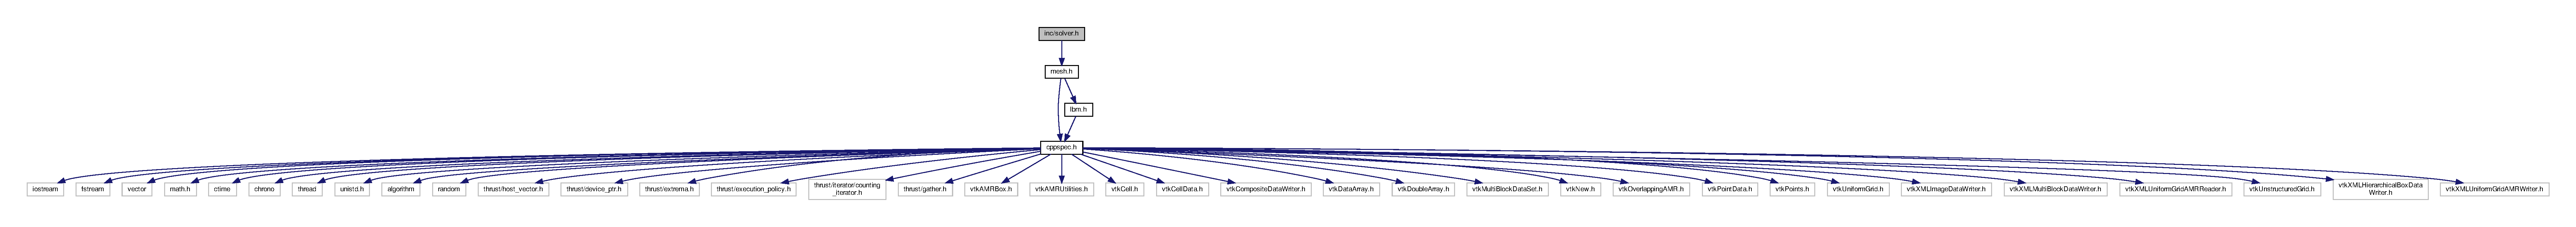
\includegraphics[width=350pt]{solver_8h__incl}
\end{center}
\end{figure}
This graph shows which files directly or indirectly include this file\+:
\nopagebreak
\begin{figure}[H]
\begin{center}
\leavevmode
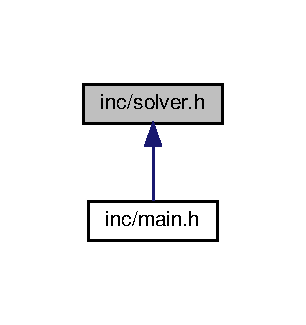
\includegraphics[width=147pt]{solver_8h__dep__incl}
\end{center}
\end{figure}
\subsection*{Classes}
\begin{DoxyCompactItemize}
\item 
class \hyperlink{classSolver}{Solver}
\item 
class \hyperlink{classSolver__LBM}{Solver\+\_\+\+L\+BM}
\end{DoxyCompactItemize}

%--- End generated contents ---

% Index
\backmatter
\newpage
\phantomsection
\clearemptydoublepage
\addcontentsline{toc}{chapter}{Index}
\printindex

\end{document}
